\documentclass[twoside, a3paper]{report}
\usepackage[utf8]{inputenc}
\usepackage[T2A]{fontenc}
\usepackage{graphicx}
\usepackage{geometry}
\usepackage{lipsum}
\usepackage{amsmath, amsthm, amsfonts, amssymb}
\usepackage{tikz, pgfplots}
\usetikzlibrary{calc}
\usetikzlibrary{positioning}
\usetikzlibrary{shapes.geometric}
\usetikzlibrary {arrows.meta}
\usepackage{titlesec}
\usepackage{listings}
\usepackage{xcolor}
\usepackage{etoolbox}
\usepackage{lipsum}
\usepackage{latexsym}
%\usepackage[OT1]{fontenc}








\lstloadlanguages{C,C++,csh,Java}

\definecolor{red}{rgb}{0.6,0,0} 
\definecolor{blue}{rgb}{0,0,0.6}
\definecolor{green}{rgb}{0,0.8,0}
\definecolor{cyan}{rgb}{0.0,0.6,0.6}

\lstset{
	language=csh,
	basicstyle=\footnotesize\ttfamily,
	numbers=left,
	numberstyle=\tiny,
	numbersep=5pt,
	tabsize=2,
	extendedchars=true,
	breaklines=true,
	frame=b,
	stringstyle=\color{blue}\ttfamily,
	showspaces=false,
	showtabs=false,
	xleftmargin=17pt,
	framexleftmargin=17pt,
	framexrightmargin=5pt,
	framexbottommargin=4pt,
	commentstyle=\color{green},
	morecomment=[l]{//}, %use comment-line-style!
	morecomment=[s]{/*}{*/}, %for multiline comments
	showstringspaces=false,
	morekeywords={ abstract, event, new, struct,
		as, explicit, null, switch,
		base, extern, object, this,
		bool, false, operator, throw,
		break, finally, out, true,
		byte, fixed, override, try,
		case, float, params, typeof,
		catch, for, private, uint,
		char, foreach, protected, ulong,
		checked, goto, public, unchecked,
		class, if, readonly, unsafe,
		const, implicit, ref, ushort,
		continue, in, return, using,
		decimal, int, sbyte, virtual,
		default, interface, sealed, volatile,
		delegate, internal, short, void,
		do, is, sizeof, while,
		double, lock, stackalloc,
		else, long, static,
		enum, namespace, string},
	keywordstyle=\color{blue},
	identifierstyle=\color{black},
	stringstyle=\color{red},
	backgroundcolor=\color{white},
}

\usepackage{caption}
\DeclareCaptionFont{white}{\color{white}}
\DeclareCaptionFormat{listing}{\colorbox{blue}{\parbox{\textwidth}{\hspace{15pt}#1#2#3}}}
\captionsetup[lstlisting]{format=listing,labelfont=white,textfont=white, singlelinecheck=false, margin=0pt, font={bf,footnotesize}}

\newtoggle{InString}{}% Keep track of if we are within a string
\togglefalse{InString}% Assume not initally in string

\newcommand*{\ColorIfNotInString}[1]{\iftoggle{InString}{#1}{\color{red}#1}}%
\newcommand*{\ProcessQuote}[1]{#1\iftoggle{InString}{\global\togglefalse{InString}}{\global\toggletrue{InString}}}%
\lstset{literate=%
	{"}{{{\ProcessQuote{"}}}}1% Disable coloring within double quotes
	{'}{{{\ProcessQuote{'}}}}1% Disable coloring within single quote
	{0}{{{\ColorIfNotInString{0}}}}1
	{1}{{{\ColorIfNotInString{1}}}}1
	{2}{{{\ColorIfNotInString{2}}}}1
	{3}{{{\ColorIfNotInString{3}}}}1
	{4}{{{\ColorIfNotInString{4}}}}1
	{5}{{{\ColorIfNotInString{5}}}}1
	{6}{{{\ColorIfNotInString{6}}}}1
	{7}{{{\ColorIfNotInString{7}}}}1
	{8}{{{\ColorIfNotInString{8}}}}1
	{9}{{{\ColorIfNotInString{9}}}}1
}







\title{Анализ задачи распределения ресурсов при помощи конвейеров и маршрутизаторов}
\author{Prishelets}
\date{2026}


%\newgeometry{
%	top=0.25in,
%	bottom=0.75in,
%	outer=0.5in,
%	inner = 1.5in,
%}

\newgeometry{
	top    = 15pt,
	bottom = 40pt,
	outer  = 25pt,
	inner  = 80pt,
}


\titleformat{\chapter}[display]{\normalfont\huge\bfseries}{\chaptertitlename\ \thechapter}{20pt}{\Huge}
\titlespacing*{\chapter}{0pt}{0pt}{40pt}




\begin{document}

\begin{titlepage}
	\begin{tikzpicture}[remember picture, overlay]
		\node[inner sep=0pt, anchor=center] at (current page.center) {
			
\includegraphics[width=\paperwidth, height=\paperheight]{обложка.png}
		};
	\end{tikzpicture}
\end{titlepage}

% Для удобного чтения закомментил, но при печати надо разкоментить, чтобы страницы легли как надо (наверное, а может и нет... хз)
% \newpage
% \thispagestyle{empty}
% \mbox{}
\newpage

\maketitle

\chapter*{Введение}
\

В данной работе рассматривается задача распределения ресурсов при помощи конвейеров и маршрутизаторов -- в основном, на основе компьютерной игры Satisfactory. Рассматриваются типизация, реализация и взаимодействие друг с другом таких объектов, как: конвейерная лента, конвейерный соединитель, конвейерный разъединитель, и прочие их надстройки. Рассматривается как общее решение задачи распределения ресурсов, так и некоторые частные задачи.

\

\textbf{Обоснование выбранного метода}: в мире, помимо используемого в основном в данной работе метода "балансировки"%
\footnote{Ресурсы равномерно распределяются между всеми выходами, обычно выполняется, как степенное дерево}
существуют и методы "шины"%
\footnote{Есть одна конвейерная лента, а потребители стоят вряд параллельно ей. Первый потребитель получает половину ресурсов, второй -- четверь, и так далее... Как только один потребитель забивается -- следущий принимает уже не половину от него, а остаток}
(самого популярного в мире), и даже некоторые экзотичесике методы, которые я не буду сейчас описывать... "Балансировка" мне нравится тем, что это самый контролируемый метод: строитель чётко знает, где сколько едет, на какую нагрузку что рассчитанно, и так далее. Так же этот метод имеет наибольшую скорость запуска производства: все ресурсы приходят чуть ли не одновременно к потребителям, в то время, как на шине ресурсы заполняют потребителей по одному, начиная с самого начала, а конечные потребители долгое время "голодают".

\

\textbf{К читателю}: Это моя первая работа -- так что не судите строго. любая конструктивная критика будет принята, проанализированна, и поможет улучшить имеющиеся наработки. За некоторое (довольно большое) число таких итераций, мы добьёмся качественой работы.


\tableofcontents


\chapter{Терминология}

\section{Конвейер}

\noindent Конвейер -- средство непрерывной перевозки ресурсов между двумя любыми точками.

\

\noindent Каждый конвейер характеризуется:
\begin{itemize}
	\item Формой
	
		Описывается системой уравнений:
		$$\vec{r}(t) = \begin{cases} x_1 = x_1(t) \\ \vdots \\ x_n = x_n(t) \\ \end{cases} \subseteq \ \mathbb{R}^n$$
		В частности: $\mathbb{R}^3$ (Satisfactory) или $\mathbb{R}^2$ (Factoro)
	
	\item Функцией распределения динамики скорости вдоль конвейера 
		
		$v(\vec{r}, t) \cong v(t_{\text{path}}, t_{\text{time}}) = v\left(\vec{t}\right)$
	
	\item Начальной $\vec{r}(0)$ и конечной $\vec{r}(t\to\text{max})$ точкой
\end{itemize}


\vspace{0.3in}


На чертежах обозначается кривой, либо отрезком, соединяющим пару точек. Может иметь стрелки для указания направления движения, а рядом может подписываться пропускная способность:

\vspace{0.5in}


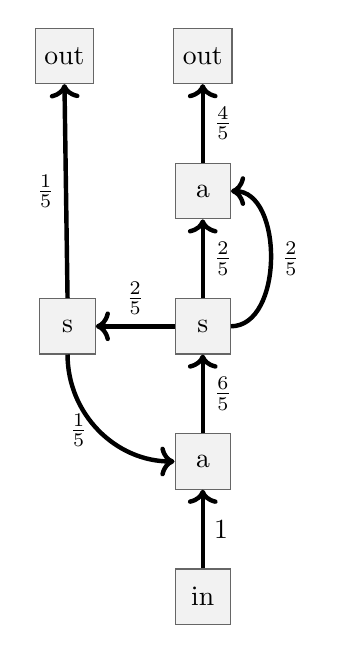
\begin{tikzpicture}[
	s/.style={rectangle, draw=black!60, fill=black!5, thin, minimum size=20},
	a/.style={rectangle, draw=black!60, fill=black!5, thin, minimum size=20},
	o/.style={rectangle, draw=black!60, fill=black!5, thin, minimum size=20},
	]
	
	%Nodes
	\node[a]    (a1)                          	{a};
	\node[s]    (s1)        [above = of a1]     {s};
	\node[s]    (s2)        [left = of s1]      {s};
	\node[o]	(in1)		[below = of a1]		{in};
	\node[a]    (a2)        [above = of s1]   	{a};
	\node[o]	(out1)		[above = of a2]		{out};
	\node[o]	(out2)		[left = of out1]	{out};
	
	%Lines
	\draw[->, ultra thick] (in1.north) to node[right] 	 			 {$\boldmath{ 1 }$} 		  (a1.south);
	\draw[->, ultra thick] (a1.north)  to node[right] 	 		 	 {$\boldmath{ \frac{6}{5} }$} (s1.south);
	\draw[->, ultra thick] (s1.west)   to node[above] 	 		 	 {$\boldmath{ \frac{2}{5} }$} (s2.east);
	\draw[->, ultra thick] (s2) 	   to[bend left=-45] node[left]  {$\boldmath{ \frac{1}{5} }$} (a1);
	\draw[->, ultra thick] (s1.north)  to node[right] 				 {$\boldmath{ \frac{2}{5} }$} (a2.south);
	\draw[->, ultra thick] (s1) 	   to[bend right=90] node[right] {$\boldmath{ \frac{2}{5} }$} (a2);
	\draw[->, ultra thick] (a2.north)  to node[right] 	 			 {$\boldmath{ \frac{4}{5} }$} (out1.south);
	\draw[->, ultra thick] (s2.north)  to node[left]	 			 {$\boldmath{ \frac{1}{5} }$} (out2.south);
\end{tikzpicture}






\newpage

\section{Конвейерный разъединитель}

\

Конвейерный разъединитель (англ: splitter) -- устройство, разъединяющее одну конвейерную ленту на несколько других.

\

\noindent Каждый конвейерный разъединитель характеризуется:

\begin{itemize}
	\item числом выходных лент $n \in \mathbb{N}$
	
	\item правилами вывода: $\{ \varphi_i \}$
\end{itemize}

\vspace{0.15in}

%На чертежах обозначается фигурой (обычно, квадрат) с буквой "s" (splitter), к которому с одной стороны подводится конвейер, а с остальных сторон -- конвейеры отводятся:
%Будем обозначать фигурой синего цвета, а буквой (s, или f характеризовать конвкретный тип), а на выходах специальными метками обозначать правило $\varphi_i$.
На чертежах обозначается синей фигурой (обычно, квадрат). Буква внутри ("s" -- splitter, "f" -- filter, итд) характеризует подтип устройства. На выходах могут находиться специальные метки, обозначающие правила вывода $\varphi_i$. К разъединителю с одной стороны подводится конвейер, а со всех остальных -- конвейеры отводятся.


\vspace{0.4in}


\begin{minipage}{0.3\textwidth}
	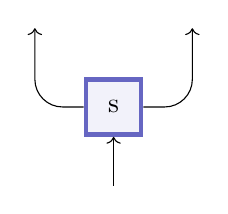
\begin{tikzpicture}[
		s/.style={rectangle, draw=blue!60, fill=blue!5, ultra thick, minimum size=20},
		r/.style = {->, thin, rounded corners=10pt},
		]
		
		\node[s]    (s)		at	(0, 0)	{s};
		\draw[r]	(0,-1)	to	(s);
		\draw[r]	(s)		-|	(-1, 1);
		\draw[r]	(s)		-|	(1, 1);
	\end{tikzpicture}
\end{minipage}
\begin{minipage}{0.3\textwidth}
	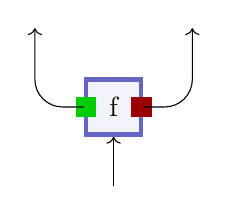
\begin{tikzpicture}[
		s/.style = {rectangle, draw=blue!60,	fill=blue!5,	ultra thick, minimum size=20},
		a/.style = {rectangle, draw=black!60,	fill=black!5,		  thin,  minimum size=20},
		o/.style = {rectangle, draw=black!60,	fill=black!5,		  thin,  minimum size=20},
		q/.style = {rectangle, draw,			fill, 						 minimum size=0.25cm},
		r/.style = {->, thin, rounded corners=10pt},
		l/.style = {	thin, rounded corners=10pt},
		]
		
		
		% === === Nodes === ===
		\node[s]		(f)		at	(0, 0)			{f};
		\node[q, red]	(n3)	at	(0.35, 0)		{};
		\node[q, green]	(n4)	at	(-0.35, 0)		{};
		
		\draw[r]		(f)		-|	(-1, 1);
		\draw[r]		(f)		-|	(1, 1);
		\draw[r]		(0, -1)	to	(f);
		
	\end{tikzpicture}
\end{minipage}

















\vspace{0.5in}

\section{Конвейерный соединитель}

\

Конвейерный соединитель (англ: adder/merger) -- устройство, соединяющее несколько входных лент в одну.

\

\noindent Каждый конвейерный соединитель характеризуется

\begin{itemize}
	\item Числом входных лент $n \in \mathbb{N}$
	
	\item Правилами приёма(ввода): $\{ \varphi_i \}$
\end{itemize}


\vspace{0.15in}

%На чертежах обозначается фигурой (обычно, квадратом) с буквой "a" (adder), к которому с одной стороны подводится конвейер на вывод, а с остальных сторон -- конвейеры входят:
На чертежах обозначается красной фигурой (обычно, квадрат). Буква внутри ("a" -- adder, "p" -- priority, итд) характеризует подтип устройства. На входах могут находиться специальные метки, обозначающие правила ввода $\varphi_i$. От соединителя с одной стороны конвейер отводится, а к остальным -- подводятся.


\vspace{0.4in}


\begin{minipage}{0.3\textwidth}
	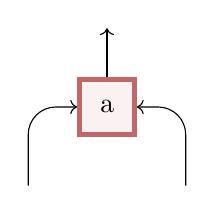
\begin{tikzpicture}[
		a/.style={rectangle, draw=red!60, fill=red!5, ultra thick, minimum size=20},
		r/.style = {->, thin, rounded corners=10pt},
		]
		
		%Nodes
		\node[a]    (a)			at	(0, 0)	{a};
		\draw[r]	(-1, -1)	|-	(a);
		\draw[r]	(1, -1)		|-	(a);
		\draw[r]	(a)			to	(0, 1);
	\end{tikzpicture}
\end{minipage}
\begin{minipage}{0.3\textwidth}
	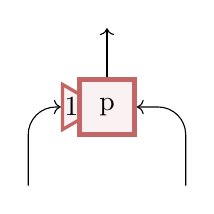
\begin{tikzpicture}[
		a/.style={rectangle, draw=red!60, fill=red!5, ultra thick, minimum size=20},
		r/.style = {->, thin, rounded corners=10pt},
		]
		
		
		\node[
			draw=red!60, fill=red!5, very thick,
			regular polygon, regular polygon sides=3, 
			rotate=-90, minimum size=0.5cm
			] 
					(tri)	at  (-0.4, 0) {};
		\node[a]	(p)		at	(0, 0)			{p};
		\node				at	(-0.45, 0)		{$1$};
		
		\draw[r]	(-1, -1)	|-	(tri);
		\draw[r]	(1, -1)		|-	(p);
		\draw[r]	(p)			to	(0, 1);
	\end{tikzpicture}
\end{minipage}
\begin{minipage}{0.3\textwidth}
	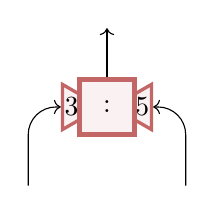
\begin{tikzpicture}[
		a/.style={rectangle, draw=red!60, fill=red!5, ultra thick, minimum size=20},
		r/.style = {->, thin, rounded corners=10pt},
		]
		
		
		\node[
			draw=red!60, fill=red!5, very thick,
			regular polygon, regular polygon sides=3, 
			rotate=-90, minimum size=0.5cm
			] 
					(tri1)	at  (-0.4, 0) {};
		\node				at	(-0.45, 0)		{$3$};
		
		\node[
			draw=red!60, fill=red!5, very thick,
			regular polygon, regular polygon sides=3, 
			rotate=90, minimum size=0.5cm
			] 
					(tri2)	at  (0.4, 0) {};
		\node				at	(0.45, 0)		{$5$};
		
		\node[a]	(p)		at	(0, 0)			{:};
		
		\draw[r]	(-1, -1)	|-	(tri1);
		\draw[r]	(1, -1)		|-	(tri2);
		\draw[r]	(p)			to	(0, 1);
	\end{tikzpicture}
\end{minipage}








\vspace{0.4in}

Также существуют специальные объекты, которые не являются ни соединителями ни разъединителями в прямом смысле: 
они как бы перемешивают ресурсы между конвейерами. Имеют они, соответственно по два входа и выхода:






\vspace{0.4in}

\begin{minipage}{0.315\textwidth}
	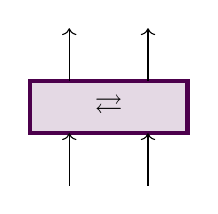
\begin{tikzpicture}[
		r/.style = {->, thin, rounded corners=10pt},
		]
		
		\draw[draw={rgb:red,255;blue,255},	fill={rgb:red!15,255;blue!15,255}, ultra thick]	(-1, 0.333)	rectangle node {$\rightleftarrows$} (1, -0.333);
		\draw[r]	(-0.5, -1)		to	(-0.5, -0.333);
		\draw[r]	(0.5, -1)		to	(0.5, -0.333);
		\draw[r]	(-0.5, 0.333)	to	(-0.5, 1);
		\draw[r]	(0.5, 0.333)	to	(0.5, 1);
	\end{tikzpicture}
\end{minipage}
\begin{minipage}{0.3\textwidth}
	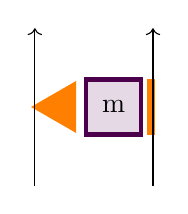
\begin{tikzpicture}[
		s/.style = {rectangle, draw={rgb:red,255;blue,255},	fill={rgb:red!15,255;blue!15,255},	ultra thick, minimum size=20},
		r/.style = {->, thin, rounded corners=10pt},
		]
		
		
		% === === Nodes === ===
		\node[s]		(m)		at	(0, 0)			{m};
		\draw[draw=orange,	fill=orange, ultra thick]	(0.45, 0.333)	rectangle (0.5, -0.333);
		\node[
		draw=orange, fill=orange, very thick,
		regular polygon, regular polygon sides=3, 
		rotate=90, 
		minimum size=0.12cm, inner sep=0.12cm, outer sep=0.12cm,
		] 
		(tri1) at (-0.667, 0) 		{};
		
		\draw[r]	(0.5, -1)	to	(0.5, 1);
		\draw[r]	(-1, -1)	to	(-1, 1);
		
	\end{tikzpicture}
\end{minipage}








\chapter{Быстрые системы}

\section{Введение}

\noindent Рассмотрим следующую систему:

\begin{itemize}
	\item Конвейеры имеют всюду равномерную скорость $v$, притом достаточно большую, чтобы можно было пренебречь взаимодействием между ресурсами, и преодолеваемыми ими расстояниями (а соответственно -- и временем)
	
	\item Конвейерные разъединители работают по следующим правилам:
		\begin{itemize}
			\item Всевозможные их числа выходов образуют множество $\mathbb{T} = \{ t_1, ..., t_n \}$
			\item Правило вывода: чередовать ресурс между выходами 
				
				Схема очерёдности:
				
				\vspace{0.25in}
				
				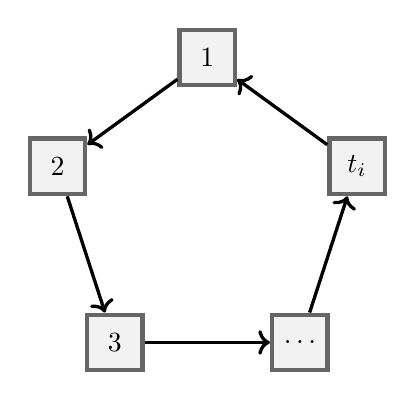
\begin{tikzpicture}[
					a/.style={rectangle, draw=black!60, fill=black!5, ultra thick, minimum size=20}
					]
					
					%Nodes
					\node[a] (1)   at (0, 2) 		   {$1$};
					\node[a] (2)   at (-1.902, 0.618)  {$2$};
					\node[a] (3)   at (-1.176, -1.618) {$3$};
					\node[a] (etc) at (1.176, -1.618)  {$\ldots$};
					\node[a] (i)   at (1.902, 0.618)   {$t_i$};
					
					%Lines
					\draw[->, very thick] (1) to (2);
					\draw[->, very thick] (2) to (3);
					\draw[->, very thick] (3) to (etc);
					\draw[->, very thick] (etc) to (i);
					\draw[->, very thick] (i) to (1);
				\end{tikzpicture}
				
			\item При этом распределение происходит мгновенно: как только ресурс заходит -- так только и выходит
				
		\end{itemize}
		
	\item Конвейерный соединитель может принимать любое число ресурсов, и мгновенно объединяет их в один конвейер (очерёдность не важна, т.к. ресурсы друг с другом не взаимодействуют)
	
\end{itemize}





\vspace{0.25in}

\noindent Всвязи с мгновенностью распределений, назовём такую систему "быстрой".

\vspace{0.4in}

\noindent В быстрых системах определён следующий набор действий:

\begin{itemize}
	\item Разделение (англ: splitting/chopping) -- разделение одного конвейера на $n$ равных частей
	
		%\begin{tikzpicture}[
		%	o/.style={rectangle, draw=green!60, fill=green!5, thick, minimum size=20},
		%	s/.style={rectangle, draw=blue!60,  fill=blue!5,  thick, minimum size=20},
		%	r/.style = {->, thick, rounded corners=10pt}
		%	]
		%	
		%	%Nodes
		%	\node[o]	(in)	at	(-2, 0)	{in};
		%	\draw[draw=blue!60,	fill=blue!5] (-0.5, 1) rectangle node {$s$} (0.5, -1);
		%	\node[o]	(out1)	at	(2, 2)	{$1$};
		%	\node[o]	(oute)	at	(2, 0)	{$\ldots$};
		%	\node[o]	(outn)	at	(2, -2)	{$n$};
		%	
		%	%Lines
		%	\draw[r]	(in.east)	to	node[above]			{$n$}	(-0.5, 0);
		%	\draw[r]	(0, 1) 		|-	node[below right]	{$1$}	(out1.west);
		%	\draw[r]	(0.5, 0) 	to	node[above]			{$1$}	(oute.west);
		%	\draw[r]	(0, -1) 	|-	node[above right]	{$1$}	(outn.west);
		%	
		%\end{tikzpicture}
		
	
	\item Соединение (англ: merging) -- соединение $n$ конвейеров в один
		
	\item Возврат (англ: re-looping/re-cycling) -- сначала отделение некоторой части потока, а затем соединение этой части с началом самого потока
	
		Пример:
		
		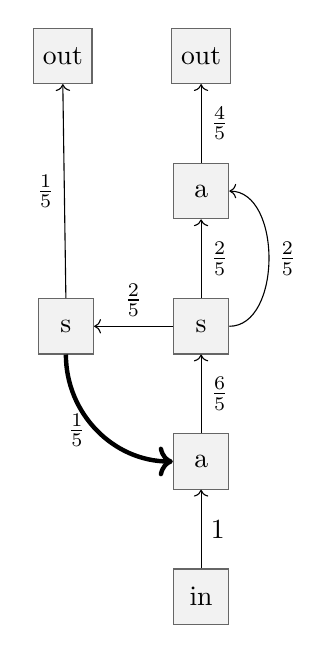
\begin{tikzpicture}[
			s/.style={rectangle, draw=black!60, fill=black!5, thin, minimum size=20},
			a/.style={rectangle, draw=black!60, fill=black!5, thin, minimum size=20},
			o/.style={rectangle, draw=black!60, fill=black!5, thin, minimum size=20},
			]
			
			%Nodes
			\node[a]    (a1)                          	{a};
			\node[s]    (s1)        [above = of a1]     {s};
			\node[s]    (s2)        [left = of s1]      {s};
			\node[o]	(in1)		[below = of a1]		{in};
			\node[a]    (a2)        [above = of s1]   	{a};
			\node[o]	(out1)		[above = of a2]		{out};
			\node[o]	(out2)		[left = of out1]	{out};
			
			%Lines
			\draw[->, thin] (in1.north) to node[right] 	 			  {$1$} 		  (a1.south);
			\draw[->, thin] (a1.north)  to node[right] 	 		 	  {$\frac{6}{5}$} (s1.south);
			\draw[->, thin] (s1.west)   to node[above] 	 		 	  {$\frac{2}{5}$} (s2.east);
			\draw[->, ultra thick] (s2) to[bend left=-45] node[left]  {$\frac{1}{5}$} (a1);
			\draw[->, thin] (s1.north)  to node[right] 				  {$\frac{2}{5}$} (a2.south);
			\draw[->, thin] (s1) 	    to[bend right=90] node[right] {$\frac{2}{5}$} (a2);
			\draw[->, thin] (a2.north)  to node[right] 	 			  {$\frac{4}{5}$} (out1.south);
			\draw[->, thin] (s2.north)  to node[left]	 			  {$\frac{1}{5}$} (out2.south);
		\end{tikzpicture}
		
	\item Отделение%
	\footnote{\textbf{Раз}деление и \textbf{от}деление отличаются тем, что \textbf{Раз}деление -- это построение n-арного дерева; а \textbf{от}деление -- это построение второй ветви, по которой едет заданное число ресурсов. Более заметно это различие в английской терминологии, а в русской различие заключается лишь приставкой...}
	(англ: separating) -- набор из последовательных и параллельных разделений, соединений и возвратов, с целью отделения заданой части $q_1$ ресурсов от изначальной конвейерной ленты, перевозящей $q_0$ ресурсов ($q_1 < q_0$)
		
		
\end{itemize}














\vspace{0.5in}


Назовём все числа вида $s = \prod_{i=1}^n t_i^{a_i}$ , где $a_i \in \mathbb{N}_0$ "стандартными". Тогда каждое число, \underline{обратное стандартному}%
\footnote{Будем называть такие числа единичными стандартными, или просто единичными. А если в числителе стоит не единица -- то будем называть их стандартными долями.} 
может быть получено, как отделение от конвейера в 1 при помощи смеси $t_1$-арного,~...~,~и $t_n$-арного деревьев.






\vspace{0.5in}

\section{Теорема о числе перестановок}

\

Для множества $\mathbb{T} = \{2, 3\}$ , число $2^13^1=6$ является стандартным, тогда $1/6$ является единичной дробью, её можно получить двумя способами:





\vspace{0.25in}

\begin{minipage}{0.4\textwidth}
	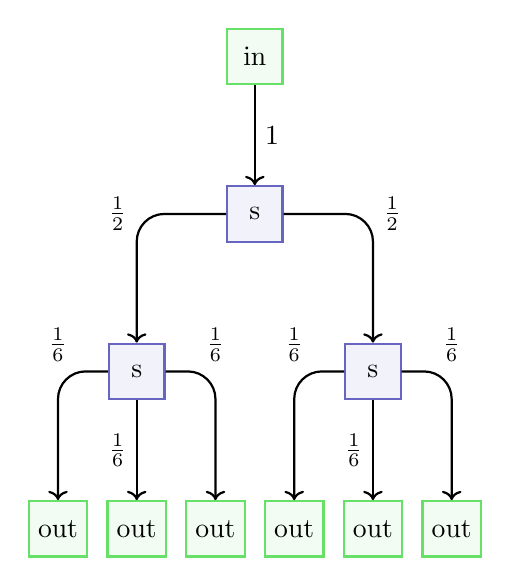
\begin{tikzpicture}[
		s/.style = {rectangle, draw=blue!60, fill=blue!5, thick, minimum size=20},
		a/.style = {rectangle, draw=red!60, fill=red!5, thick, minimum size=20},
		o/.style = {rectangle, draw=green!60, fill=green!5, thick, minimum size=20},
		r/.style = {->, thick, rounded corners=10pt}
		]
		
		%Nodes
		\node[o]	(in1)	at (0, 2)		{in};
		\node[s]	(s1)	at (0, 0)		{s};
		\node[s]	(s2)    at (-1.5, -2)	{s};
		\node[s]	(s3)    at (1.5, -2)	{s};
		\node[o]	(out1)	at (-2.5, -4)	{out};
		\node[o]	(out2)	at (-1.5, -4)	{out};
		\node[o]	(out3)	at (-0.5, -4)	{out};
		\node[o]	(out4)	at (0.5, -4)	{out};
		\node[o]	(out5)	at (1.5, -4)	{out};
		\node[o]	(out6)	at (2.5, -4)	{out};
		
		%Lines
		\draw[->, thick] (in1.south) to node[right] {$1$} 			(s1.north);
		\draw[->, thick] (s2.south)  to node[left]  {$\frac{1}{6}$} (out2.north);
		\draw[->, thick] (s3.south)  to node[left]  {$\frac{1}{6}$} (out5.north);
		
		\draw[r] (s1.west) -| node[left]   {$\frac{1}{2}$} (s2.north);
		\draw[r] (s1.east) -| node[right]  {$\frac{1}{2}$} (s3.north);
		\draw[r] (s2.west) -| node[above]  {$\frac{1}{6}$} (out1.north);
		\draw[r] (s2.east) -| node[above]  {$\frac{1}{6}$} (out3.north);
		\draw[r] (s3.west) -| node[above]  {$\frac{1}{6}$} (out4.north);
		\draw[r] (s3.east) -| node[above]  {$\frac{1}{6}$} (out6.north);
		
	\end{tikzpicture}
\end{minipage}
\hspace{50pt}
\begin{minipage}{0.4\textwidth}
	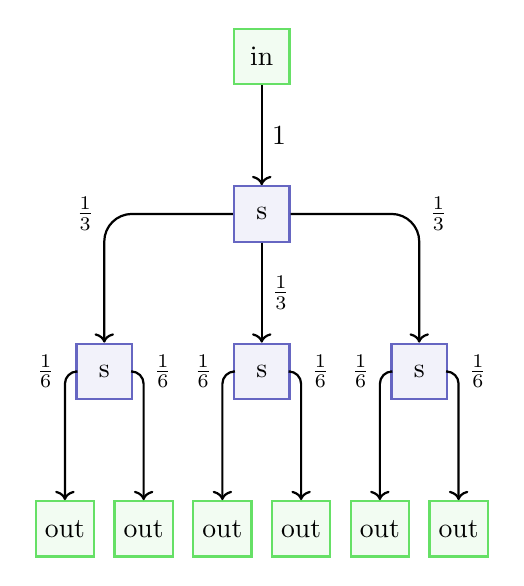
\begin{tikzpicture}[
		s/.style={rectangle, draw=blue!60, fill=blue!5, thick, minimum size=20},
		a/.style={rectangle, draw=red!60, fill=red!5, thick, minimum size=20},
		o/.style={rectangle, draw=green!60, fill=green!5, thick, minimum size=20},
		r1/.style = {->, thick, rounded corners=10pt},
		r/.style = {->, thick, rounded corners=4.5pt}
		]
		
		%Nodes
		\node[o]	(in1)	at (0, 2)		{in};
		\node[s]	(s1)	at (0, 0)		{s};
		\node[s]	(s2)	at (-2, -2)		{s};
		\node[s]	(s3)    at (0, -2)		{s};
		\node[s]	(s4)    at (2, -2)		{s};
		\node[o]	(out1)	at (-2.5, -4)	{out};
		\node[o]	(out2)	at (-1.5, -4)	{out};
		\node[o]	(out3)	at (-0.5, -4)	{out};
		\node[o]	(out4)	at (0.5, -4)	{out};
		\node[o]	(out5)	at (1.5, -4)	{out};
		\node[o]	(out6)	at (2.5, -4)	{out};
		
		%Lines
		\draw[->, thick] (in1.south) to node[right] {$1$} 			(s1.north);
		\draw[r1] 		 (s1.west) 	 -| node[left]  {$\frac{1}{3}$} (s2.north);
		\draw[->, thick] (s1.south)  to node[right] {$\frac{1}{3}$} (s3.north);
		\draw[r1] 		 (s1.east)   -| node[right] {$\frac{1}{3}$} (s4.north);
		
		\draw[r] (s2.west) -| node[left]  {$\frac{1}{6}$} (out1.north);
		\draw[r] (s2.east) -| node[right] {$\frac{1}{6}$} (out2.north);
		\draw[r] (s3.west) -| node[left]  {$\frac{1}{6}$} (out3.north);
		\draw[r] (s3.east) -| node[right] {$\frac{1}{6}$} (out4.north);
		\draw[r] (s4.west) -| node[left]  {$\frac{1}{6}$} (out5.north);
		\draw[r] (s4.east) -| node[right] {$\frac{1}{6}$} (out6.north);
		
	\end{tikzpicture}
\end{minipage}

\newpage

Как можем заметить, дробь одна, а варианта её воспроизводства -- два. Отсюда сформулируем теорему:

\

Любую единичную дробь, инициализированную числом  $s = \prod_{i=1}^n t_i^{a_i}$ можно построить числом способов, равным числу перестановок его сомножителей:

$$
	\text{P}\left[ \sum_{i=1}^{n} a_i \right] \left( a_1, a_2, \ldots, a_n \right) 
	=
	\dfrac{\left[ \sum\limits_{i=1}^{n} a_i \right]!}{\prod\limits_{i=1}^{n} \left( a_i! \right)}
$$











\vspace{0.5in}

\section{Теорема о делимости}

\

Если некоторую стандартную долю конвейера $\frac{a}{s} \ (a < s)$ возвратить в его начало -- то на участке до начала отделения пойдёт $q_0 + \frac{a}{s}\cdot q_0$ , после второй рекурсии -- $q_0 + \frac{a}{s}\cdot \left( q_0 + \frac{a}{s}\cdot q_0 \right)$ , и так далее.

\

\noindent Таким образом, в конечном итоге по данному участку будет идти:

$$\sum_{i=0}^{\infty} q_0 \cdot \left( \frac{a}{s} \right)^i = q_0 \cdot \frac{1}{1-\frac{a}{s}} = q_0\cdot\frac{s}{s-a}$$

\

Так как $a$ можно выбрать произвольное -- то от конвейера можно отделить даже не стандартную долю.

\vspace{0.3in}

\noindent Обозначим операцию преобразования дроби $\frac{a}{s}$ в дробь $\frac{a}{b} \ (b \le s)$ за:

\begin{align*}
	&\frac{a}{s} - \frac{s-b}{s} := \frac{a}{s} \cdot \frac{1}{1 - \frac{s-b}{s}} = \frac{a}{b} \\	
	&\frac{a}{s} - \frac{b}{s} := \frac{a}{s} \cdot \frac{1}{1 - \frac{b}{s}} = \frac{a}{s-b}
\end{align*}

\vspace{0.3in}

Теорема: любой единичный конвейер можно разделить на любые два положительных рациональных, в сумме дающих единицу, как рациональные доли входного конвейера при помощи операций отделения и возврата

\begin{align*}
	&\forall \ q_0, q_1, q_2 \in \mathbb{Q}^+_0 \ (q_1 + q_2 = q_0) \ : \\
	&\exists \ a, b, s \in \mathbb{N}_0 \ (a, b \le s) \ (s - \text{standart}) \ | \\
	&q_1 = \frac{a}{s} - \frac{b}{s} \ , \ q_2 = \frac{s-a-b}{s} - \frac{b}{s}
\end{align*}












\vspace{0.5in}

\section{Теорема об упрощении}

\

\noindent Назовём системы:

\begin{itemize}
	\item "простыми", если: $\forall \ t_i \in \mathbb{T} \ : \ t_i$ -- простое
		
		Пример: $\mathbb{T} = \{2, 3\}$, $\mathbb{T} = \{11, 23, 41\}$, $\mathbb{T} \subseteq \{2, 3, 5, 7, 11, 13, \ldots\}$
	
	\item "полупростыми", если: $\forall t_i, t_j \in \mathbb{T} \ : \ \gcd(t_i; \ t_j) = 1$
	
		Пример: $\mathbb{T} = \{2, 3\}$, $\mathbb{T} = \{4, 9\}$, $\mathbb{T} = \{6, 7, 25\}$
	
	\item "дублирующими", если: $\exists \ t, a, b \in \mathbb{T} \ ; \ x \in \mathbb{N}_0 \ ; \ y, z \in \mathbb{N} \ | \ t^z = a^x b^y$
	
		Пример: $\mathbb{T} = \{2, 3, 6\}$, $\mathbb{T} = \{2, 4\}$, $\mathbb{T} = \{4, 6, 9\}$
\end{itemize}

\

Теорема: любую дублирующую систему можно упростить:

\begin{align*}
	&\forall \ \mathbb{T} \ | \ \exists \ t, a, b \in \mathbb{T} \ ; \ x \in \mathbb{N}_0 \ ; \ y, z \in \mathbb{N} \ | \ t^z = a^x b^y \ : \\
	&\exists \ \mathbb{T}' = \mathbb{T} \setminus \{t \ : \ \exists \ t, a, b \in \mathbb{T} \ ; \ x \in \mathbb{N}_0 \ ; \ y, z \in \mathbb{N} \ | \ t^z = a^x b^y \} \ne \emptyset \\
	&\mathbb{T}' - \text{prime, or half-prime}
\end{align*}

\

Таким образом не имеет смысла отдельно изучать дублирующие системы, ведь для них будут верны все свойства полупростых (и простых соответственно). Однако сами по себе дублирующие сисемы могут быть удобны в решении отдельных задачь: например, если в $t = \prod_i t_i^{a_i}$, \\ $\sum_i a_i$ -- достаточно большое -- то:

\begin{enumerate}
	\item Система, реализующая единичную дробь, инициализированную данным числом, будет банально громоздкой
	\item Возможных способов реализации такой системы тоже будет много, что значительно усложняет решение задачи
\end{enumerate}

\noindent Тогда действительно проще установить готовый разветвитель, а не строить его с нуля.




\newpage

\section{Алгебра задачи}

\subsection{Теория групп}

\

Так же хочется отметить, что каждый разделитель образует циклическую группу $C_{t_i}$ -- тогда резонно сказать, что конвейер в начале своего пути является циклической группой $C_1$, а каждый раз, применяя к нему операцию разделения при помощи серии параллельных сплиттеров, мы, по сути, домножаем группу конвейера на группу сплиттера:






\vspace{0.5in}


\begin{minipage}{0.4\textwidth}
	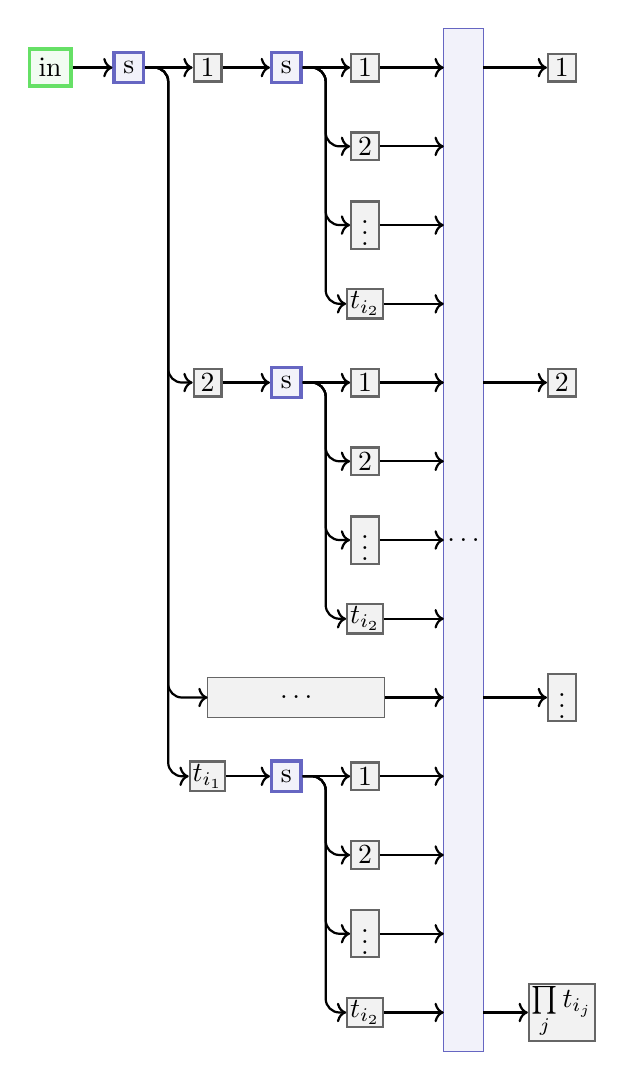
\begin{tikzpicture}[
		s/.style = {rectangle,	draw=blue!60,	fill=blue!5,	very thick, minimum size=10},
		a/.style = {rectangle,	draw=red!60,	fill=red!5,		very thick, minimum size=10},
		o/.style = {rectangle,	draw=green!60,	fill=green!5,	very thick, minimum size=10},
		t/.style = {rectangle,	draw=black!60,	fill=black!5,	thick, 		minimum size=10, inner sep=1pt},
		r/.style = {->, thick, rounded corners=5pt}
		]
		
		%Nodes
		\node[o]	(in)	at	(-3, 0)		{in};
		
		\node[s]	(s1)	at	(-2, 0)		{s};
		\node[t]	(t11)	at	(-1, 0)		{$1$};
		\node[t]	(t12)	at	(-1, -4)	{$2$};
		%\node[t]	(t1e)	at	(-1, -8)	{$\vdots$};
		\node[t]	(t1i)	at	(-1, -9)	{$t_{i_1}$};
		
		\node[s]	(s11)	at	(0, 0)		{s};
		\node[t]	(t121)	at	(1, 0)		{$1$};
		\node[t]	(t122)	at	(1, -1)		{$2$};
		\node[t]	(t12e)	at	(1, -2)		{$\vdots$};
		\node[t]	(t12i)	at	(1, -3)		{$t_{i_2}$};
		
		\node[s]	(s21)	at	(0, -4)		{s};
		\node[t]	(t221)	at	(1, -4)		{$1$};
		\node[t]	(t222)	at	(1, -5)		{$2$};
		\node[t]	(t22e)	at	(1, -6)		{$\vdots$};
		\node[t]	(t22i)	at	(1, -7)		{$t_{i_2}$};
		
		\node[s]	(si1)	at	(0, -9)		{s};
		\node[t]	(ti21)	at	(1, -9)		{$1$};
		\node[t]	(ti22)	at	(1, -10)	{$2$};
		\node[t]	(ti2e)	at	(1, -11)	{$\vdots$};
		\node[t]	(ti2i)	at	(1, -12)	{$t_{i_2}$};		
		
		% etc
		\draw[draw=blue!60,		fill=blue!5]	(2, 0.5)	rectangle node {$\ldots$} (2.5, -12.5);
		\draw[draw=black!60,	fill=black!5]	(-1, -7.75)	rectangle node {$\ldots$} (1.25, -8.25);
		
		\node[t]	(t1)	at	(3.5, 0)		{$1$};
		\node[t]	(t2)	at	(3.5, -4)		{$2$};
		\node[t]	(te)	at	(3.5, -8)		{$\vdots$};
		\node[t]	(tn)	at	(3.5, -12)		{$\prod\limits_{j} t_{i_j}$};
		
		
		
		%Lines
		\draw[r]	(in.east)	to	(s1.west);
		
		\draw[r]	(s1.east)	to	(t11.west);
		\draw[r]	(s1.east)	to	(-1.5, 0)	|-	(t12.west);
		\draw[r]	(s1.east)	to	(-1.5, 0)	|-	(-1, -8);
		\draw[r]	(s1.east)	to	(-1.5, 0)	|-	(t1i.west);
		
		\draw[r]	(t11.east)	to	(s11.west);
		\draw[r]	(s11.east)	to	(t121.west);
		\draw[r]	(s11.east)	to	(0.5, 0)	|-	(t122.west);
		\draw[r]	(s11.east)	to	(0.5, 0)	|-	(t12e.west);
		\draw[r]	(s11.east)	to	(0.5, 0)	|-	(t12i.west);
		
		\draw[r]	(t12.east)	to	(s21.west);
		\draw[r]	(s21.east)	to	(t221.west);
		\draw[r]	(s21.east)	to	(0.5, -4)	|-	(t222.west);
		\draw[r]	(s21.east)	to	(0.5, -4)	|-	(t22e.west);
		\draw[r]	(s21.east)	to	(0.5, -4)	|-	(t22i.west);
		
		\draw[r]	(t1i.east)	to	(si1.west);
		\draw[r]	(si1.east)	to	(ti21.west);
		\draw[r]	(si1.east)	to	(0.5, -9)	|-	(ti22.west);
		\draw[r]	(si1.east)	to	(0.5, -9)	|-	(ti2e.west);
		\draw[r]	(si1.east)	to	(0.5, -9)	|-	(ti2i.west);
		
		\draw[r]	(t121.east)	to	(2, 0);
		\draw[r]	(t122.east)	to	(2, -1);
		\draw[r]	(t12e.east)	to	(2, -2);
		\draw[r]	(t12i.east)	to	(2, -3);
		\draw[r]	(t221.east)	to	(2, -4);
		\draw[r]	(t222.east)	to	(2, -5);
		\draw[r]	(t22e.east)	to	(2, -6);
		\draw[r]	(t22i.east)	to	(2, -7);
		\draw[r]	(1.25, -8)	to	(2, -8);
		\draw[r]	(ti21.east)	to	(2, -9);
		\draw[r]	(ti22.east)	to	(2, -10);
		\draw[r]	(ti2e.east)	to	(2, -11);
		\draw[r]	(ti2i.east)	to	(2, -12);
		
		\draw[r]	(2.5, 0)	to	(t1.west);
		\draw[r]	(2.5, -4)	to	(t2.west);
		\draw[r]	(2.5, -8)	to	(te.west);
		\draw[r]	(2.5, -12)	to	(tn.west);
	\end{tikzpicture}
\end{minipage}
\hspace{10pt}
\begin{minipage}{0.1\textwidth}
	$$\equiv$$
\end{minipage}
\begin{minipage}{0.2\textwidth}
	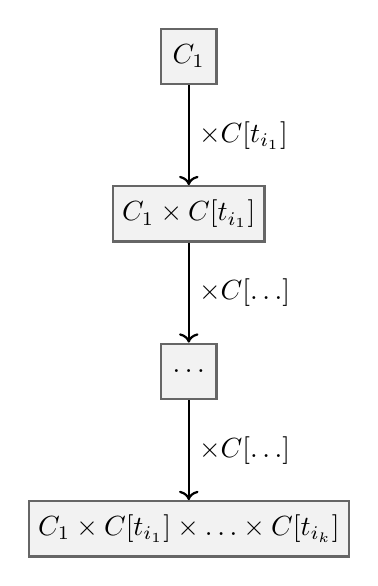
\begin{tikzpicture}[
		t/.style = {rectangle, draw=black!60, fill=black!5, thick, minimum size=20},
		r/.style = {->, thick}
		]
		
		%Nodes
		\node[t]	(1)	at	(0, 4)	{$C_1$};
		\node[t]	(2)	at	(0, 2)	{$C_1 \times C[t_{i_1}]$};
		\node[t]	(e)	at	(0, 0)	{$\ldots$};
		\node[t]	(i)	at	(0, -2)	{$C_1 \times C[t_{i_1}] \times \ldots \times C[t_{i_k}]$};
		
		%Lines
		\draw[r]	(1.south)	to	node[right]	{$\times C[t_{i_1}]$}	(2.north);
		\draw[r]	(2.south)	to	node[right]	{$\times C[\ldots]$}	(e.north);
		\draw[r]	(e.south)	to	node[right]	{$\times C[\ldots]$}	(i.north);
	\end{tikzpicture}
\end{minipage}
\hspace{10pt}
\begin{minipage}{0.1\textwidth}
	$$\equiv$$
\end{minipage}
\begin{minipage}{0.2\textwidth}
	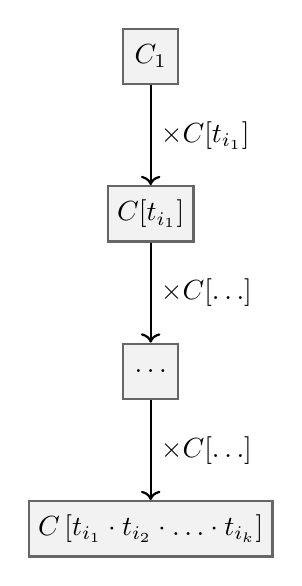
\begin{tikzpicture}[
		t/.style = {rectangle, draw=black!60, fill=black!5, thick, minimum size=20},
		r/.style = {->, thick}
		]
		
		%Nodes
		\node[t]	(1)	at	(0, 4)	{$C_1$};
		\node[t]	(2)	at	(0, 2)	{$C[t_{i_1}]$};
		\node[t]	(e)	at	(0, 0)	{$\ldots$};
		\node[t]	(i)	at	(0, -2)	{$C\left[ t_{i_1} \cdot t_{i_2} \cdot \ldots \cdot t_{i_k} \right]$};
		
		%Lines
		\draw[r]	(1.south)	to	node[right]	{$\times C[t_{i_1}]$}	(2.north);
		\draw[r]	(2.south)	to	node[right]	{$\times C[\ldots]$}	(e.north);
		\draw[r]	(e.south)	to	node[right]	{$\times C[\ldots]$}	(i.north);
	\end{tikzpicture}
\end{minipage}







\vspace{0.667in}

Тогда всё множество выходных конвейеров образует циклическую группу $C \left[ \prod_j t_{i_j} \right] \ = \ C \left[ \prod_i t_i^{a_i} \right]$. Если из них принудительно $b$ штук вернуть в начало -- то мы снова придём к теореме о делимости, и получим уменьшение периода группы: $C[s] \xrightarrow{-b} C[s-b]$






\vspace{0.5in}


\begin{minipage}{0.5\textwidth}
	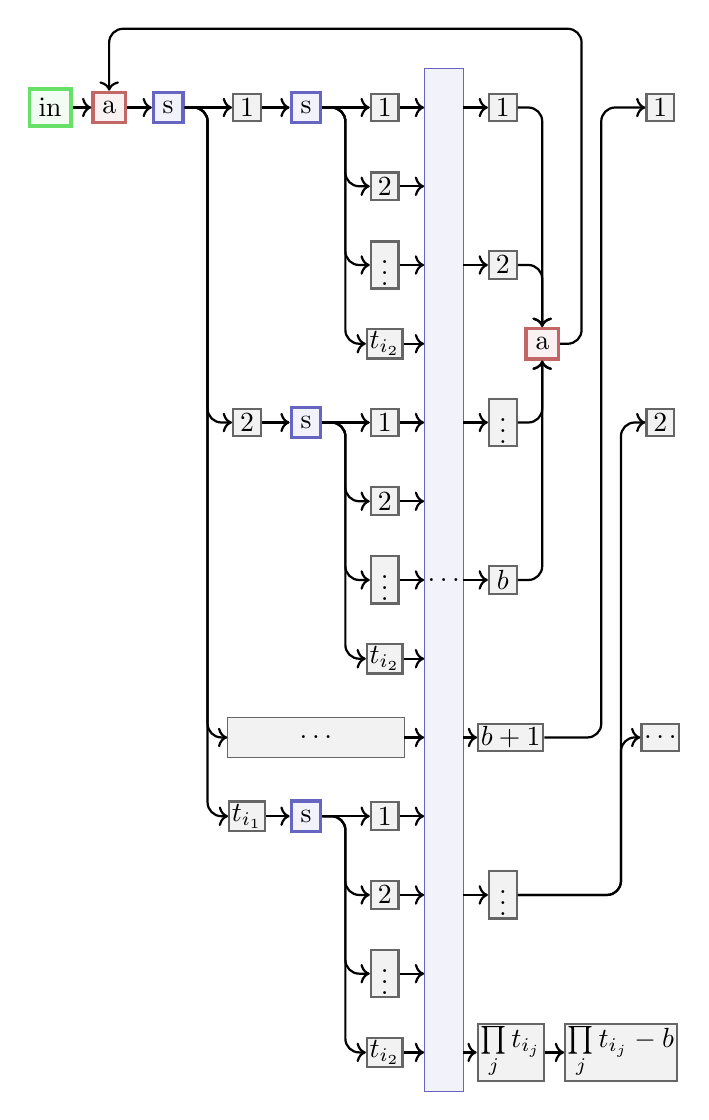
\begin{tikzpicture}[
		s/.style = {rectangle,	draw=blue!60,	fill=blue!5,	very thick, minimum size=10},
		a/.style = {rectangle,	draw=red!60,	fill=red!5,		very thick, minimum size=10},
		o/.style = {rectangle,	draw=green!60,	fill=green!5,	very thick, minimum size=10},
		t/.style = {rectangle,	draw=black!60,	fill=black!5,	thick, 		minimum size=10, inner sep=1pt},
		r/.style = {->, thick, rounded corners=5pt}
		]
		
		%Nodes
		\node[o]	(in)	at	(-3.25, 0)	{in};
		\node[a]	(a1)	at	(-2.5, 0)	{a};
		
		\node[s]	(s1)	at	(-1.75, 0)	{s};
		\node[t]	(t11)	at	(-0.75, 0)	{$1$};
		\node[t]	(t12)	at	(-0.75, -4)	{$2$};
		%\node[t]	(t1e)	at	(-1, -8)	{$\vdots$};
		\node[t]	(t1i)	at	(-0.75, -9)	{$t_{i_1}$};
		
		\node[s]	(s11)	at	(0, 0)		{s};
		\node[t]	(t121)	at	(1, 0)		{$1$};
		\node[t]	(t122)	at	(1, -1)		{$2$};
		\node[t]	(t12e)	at	(1, -2)		{$\vdots$};
		\node[t]	(t12i)	at	(1, -3)		{$t_{i_2}$};
		
		\node[s]	(s21)	at	(0, -4)		{s};
		\node[t]	(t221)	at	(1, -4)		{$1$};
		\node[t]	(t222)	at	(1, -5)		{$2$};
		\node[t]	(t22e)	at	(1, -6)		{$\vdots$};
		\node[t]	(t22i)	at	(1, -7)		{$t_{i_2}$};
		
		\node[s]	(si1)	at	(0, -9)		{s};
		\node[t]	(ti21)	at	(1, -9)		{$1$};
		\node[t]	(ti22)	at	(1, -10)	{$2$};
		\node[t]	(ti2e)	at	(1, -11)	{$\vdots$};
		\node[t]	(ti2i)	at	(1, -12)	{$t_{i_2}$};		
		
		% etc
		\draw[draw=blue!60,		fill=blue!5]	(1.5, 0.5)	rectangle node {$\ldots$} (2, -12.5);
		\draw[draw=black!60,	fill=black!5]	(-1, -7.75)	rectangle node {$\ldots$} (1.25, -8.25);
		
		\node[t]	(t1)	at	(2.5, 0)	{$1$};
		\node[t]	(t2)	at	(2.5, -2)	{$2$};
		\node[t]	(te1)	at	(2.5, -4)	{$\vdots$};
		\node[t]	(tb)	at	(2.5, -6)	{$b$};
		\node[t]	(tb+)	at	(2.6, -8)	{$b+1$};
		\node[t]	(te2)	at	(2.5, -10)	{$\vdots$};
		\node[t]	(tn)	at	(2.6, -12)	{$\prod\limits_{j} t_{i_j}$};
		
		\node[a]	(a2)	at	(3, -3)		{a};
		\node[t]	(t1`)	at	(4.5, 0)	{$1$};
		\node[t]	(t2`)	at	(4.5, -4)	{$2$};
		\node[t]	(te`)	at	(4.5, -8)	{$\ldots$};
		\node[t]	(tn`)	at	(4, -12)	{$\prod\limits_{j} t_{i_j} - b$};
	
		
		
		%Lines
		\draw[r]	(in.east)	to	(a1.west);
		\draw[r]	(a1.east)	to	(s1.west);
		
		\draw[r]	(s1.east)	to	(t11.west);
		\draw[r]	(s1.east)	to	(-1.25, 0)	|-	(t12.west);
		\draw[r]	(s1.east)	to	(-1.25, 0)	|-	(-1, -8);
		\draw[r]	(s1.east)	to	(-1.25, 0)	|-	(t1i.west);
		
		\draw[r]	(t11.east)	to	(s11.west);
		\draw[r]	(s11.east)	to	(t121.west);
		\draw[r]	(s11.east)	to	(0.5, 0)	|-	(t122.west);
		\draw[r]	(s11.east)	to	(0.5, 0)	|-	(t12e.west);
		\draw[r]	(s11.east)	to	(0.5, 0)	|-	(t12i.west);
		
		\draw[r]	(t12.east)	to	(s21.west);
		\draw[r]	(s21.east)	to	(t221.west);
		\draw[r]	(s21.east)	to	(0.5, -4)	|-	(t222.west);
		\draw[r]	(s21.east)	to	(0.5, -4)	|-	(t22e.west);
		\draw[r]	(s21.east)	to	(0.5, -4)	|-	(t22i.west);
		
		\draw[r]	(t1i.east)	to	(si1.west);
		\draw[r]	(si1.east)	to	(ti21.west);
		\draw[r]	(si1.east)	to	(0.5, -9)	|-	(ti22.west);
		\draw[r]	(si1.east)	to	(0.5, -9)	|-	(ti2e.west);
		\draw[r]	(si1.east)	to	(0.5, -9)	|-	(ti2i.west);
		
		\draw[r]	(t121.east)	to	(1.5, 0);
		\draw[r]	(t122.east)	to	(1.5, -1);
		\draw[r]	(t12e.east)	to	(1.5, -2);
		\draw[r]	(t12i.east)	to	(1.5, -3);
		\draw[r]	(t221.east)	to	(1.5, -4);
		\draw[r]	(t222.east)	to	(1.5, -5);
		\draw[r]	(t22e.east)	to	(1.5, -6);
		\draw[r]	(t22i.east)	to	(1.5, -7);
		\draw[r]	(1.25, -8)	to	(1.5, -8);
		\draw[r]	(ti21.east)	to	(1.5, -9);
		\draw[r]	(ti22.east)	to	(1.5, -10);
		\draw[r]	(ti2e.east)	to	(1.5, -11);
		\draw[r]	(ti2i.east)	to	(1.5, -12);
		
		\draw[r]	(2, 0)	to	(t1.west);
		\draw[r]	(2, -2)	to	(t2.west);
		\draw[r]	(2, -4)	to	(te1.west);
		\draw[r]	(2, -6)	to	(tb.west);
		\draw[r]	(2, -8)	to	(tb+.west);
		\draw[r]	(2, -10)	to	(te2.west);
		\draw[r]	(2, -12)	to	(tn.west);
		
		\draw[r]	(t1.east) 	-| 	(a2.north);
		\draw[r]	(t2.east) 	-| 	(a2.north);
		\draw[r]	(te1.east)	-| 	(a2.south);
		\draw[r]	(tb.east)	-| 	(a2.south);
		
		\draw[r]	(tb+.east)	to (3.75, -8) |- (t1`.west);
		\draw[r]	(te2.east)	to (4, -10) |- (t2`.west);
		\draw[r]	(te2.east)	to (4, -10) |- (te`.west);
		\draw[r]	(tn.east)	to	(tn`.west);
		
		\draw[r] 	(a2.east)	-| (3.5, 1) -| (a1.north);
	\end{tikzpicture}
\end{minipage}
\hspace{10pt}
\begin{minipage}{0.1\textwidth}
	$$\equiv$$
\end{minipage}
\begin{minipage}{0.2\textwidth}
	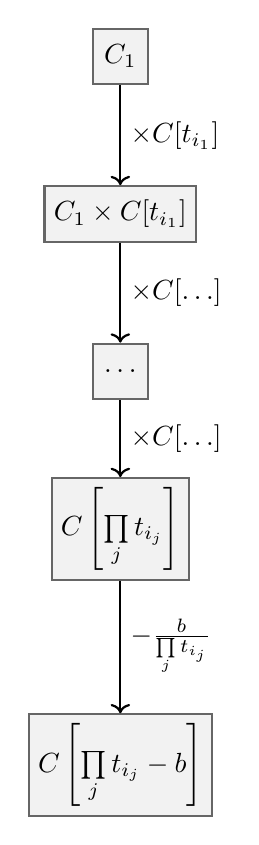
\begin{tikzpicture}[
		t/.style = {rectangle, draw=black!60, fill=black!5, thick, minimum size=20},
		r/.style = {->, thick}
		]
		
		%Nodes
		\node[t]	(1)	at	(0, 4)	{$C_1$};
		\node[t]	(2)	at	(0, 2)	{$C_1 \times C[t_{i_1}]$};
		\node[t]	(e)	at	(0, 0)	{$\ldots$};
		\node[t]	(n)	at	(0, -2)	{$C\left[ \prod\limits_{j} t_{i_j} \right]$};
		\node[t]	(*)	at	(0, -5)	{$C\left[ \prod\limits_{j} t_{i_j} - b\right]$};
		
		%Lines
		\draw[r]	(1.south)	to	node[right]	{$\times C[t_{i_1}]$}	(2.north);
		\draw[r]	(2.south)	to	node[right]	{$\times C[\ldots]$}	(e.north);
		\draw[r]	(e.south)	to	node[right]	{$\times C[\ldots]$}	(n.north);
		\draw[r]	(n.south)	to	node[right]	{$- \frac{b}{\prod\limits_{j} t_{i_j}}$}	(*.north);
	\end{tikzpicture}
\end{minipage}









\vspace{0.667in}

Схемы, приведённые справа являются биективными для любой неупрощённой диаграммы разделения, но как мы увидим далее, многие, первоначально кажущиеся сложными и громоздкими схемы -- можно довольно сильно сокращать, но тогда мы не сможем рисовать к ним данные схемы так просто. Тем более, такие схемы можно рисовать только для схем \textit{разделениея}, но не \textit{отделения}.









\vspace{0.5in}

\subsection{Теория графов}

Также хочется отметить, что, поскольку каждая схема является мультиорграфом -- то её можно описывать не в виде чертежа, а, например, в виде матрицы смежности:






%\vspace{0.5in}
\newpage

\begin{minipage}{0.25\textwidth}
	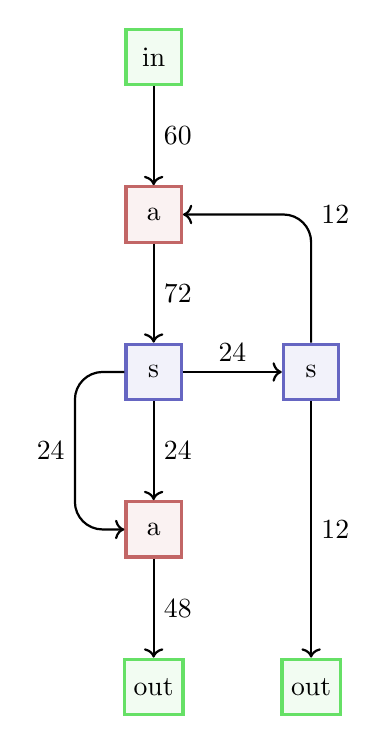
\begin{tikzpicture}[
		s/.style = {rectangle, draw=blue!60, fill=blue!5, very thick, minimum size=20},
		a/.style = {rectangle, draw=red!60, fill=red!5, very thick, minimum size=20},
		o/.style = {rectangle, draw=green!60, fill=green!5, very thick, minimum size=20},
		r/.style = {->, thick, rounded corners=10pt},
		]
		
		%Nodes
		\node[o]	(in)	at	(0, 4)	{in};
		\node[a]	(a1)	at	(0, 2)	{a};
		\node[s]	(s1)	at	(0, 0)	{s};
		\node[s]	(s2)	at	(2, 0)	{s};
		\node[a]	(a2)	at	(0, -2)	{a};
		\node[o]	(out1)	at	(0, -4)	{out};
		\node[o]	(out2)	at	(2, -4)	{out};
		
		%Lines
		\draw[r]	(in.south) 	to			node[right]	{$60$}	(a1.north);
		\draw[r]	(a1.south)	to			node[right]	{$72$}	(s1.north);
		\draw[r]	(s1.east)	to			node[above]	{$24$}	(s2.west);
		\draw[r]	(s2.north)	|-			node[right]	{$12$}	(a1.east);
		\draw[r]	(s1.west)	-| (-1, -1) node[left]	{$24$} |- (a2.west);
		\draw[r]	(s1.south)	to			node[right]	{$24$}	(a2.north);
		\draw[r]	(a2.south)	to			node[right]	{$48$}	(out1.north);
		\draw[r]	(s2.south)	to			node[right]	{$12$}	(out2.north);
	\end{tikzpicture}
\end{minipage}
\begin{minipage}{0.1\textwidth}
	$$\equiv$$
\end{minipage}
\begin{minipage}{0.4\textwidth}
	\begin{tabular}{|c|c|c|c|c|c|c|}
		\hline
		\textbackslash 
			&	a1&	a2&	s1&	s2&	out1&out2 \\
		\hline
		in&		1&	&	&	&	&	  \\
		\hline
		a1&		&	&	1&	&	&	  \\
		\hline
		a2&		&	&	&	&	1&	  \\
		\hline
		s1&		&	2&	&	1&	&	  \\
		\hline
		s2&		1&	&	&	&	&	1 \\
		\hline
		&&&&&& \\
		\hline
		in&		60&	&	&	&	&	  \\
		\hline
		a1&		&	&	72&	&	&	  \\
		\hline
		a2&		&	&	&	&	48&	  \\
		\hline
		s1&		&	24&	&	24&	&	  \\
		\hline
		s2&		12&	&	&	&	&	12\\
		\hline
	\end{tabular}
\end{minipage}




\vspace{0.5in}

Таблицу, удобства ради, давайте разделим на две части: сверху отметим обычную матрицу смежности для мультиорграфа: число в ячейке говорит о том, сколько рёбер идёт из одной вершины в другую. А снизу -- пропускную способность одного ребра.

\

Такой граф состоит из одной компоненты слабой связности, а все её компоненты сильной связности -- это области, благодоря которым происходит операция возврата. Посмотрев на полустепень исхода каждого из узлов компоненты сильной связности, можно выяснить, какой коэффициент усиления она реализует.

\

Однако матричный метод не является удобным, если все элементы $\mathbb{T}$ -- малы, а сам граф -- большой. Эффективность он преобретает, когда число выходных лент большое, а кратынх рёбер при этом мало.













\vspace{0.5in}

\subsection{Линейная алгебра}

Рассмотрим задачу перераспределения ресурсов между $n$ входами и $k$ выходами: схему перераспределения можно представить в виде матрицы:

$$
\left[
\begin{matrix}
	m_{11} & \ldots & m_{1n} \\
	\vdots & \ddots & \vdots \\
	m_{k1} & \ldots & m_{kn}
\end{matrix}
\right]
\times
\left[
\begin{matrix}
	\text{in}_1 \\
	\vdots \\
	\text{in}_n
\end{matrix}
\right]
=
\left[
\begin{matrix}
	\text{out}_1 \\
	\vdots \\
	\text{out}_k
\end{matrix}
\right]
$$

\

Рассмотрим матрицу $A \ := \ a_{ij} = \frac{\text{out}_i}{\text{in}_j}$. В ней можно выделить следующие классы значений:

%\

%Рассмотрим квадратную субматрицу $M' \subseteq M$. Если рассмотреть её диагональное решение -- то  ячейки $m_{ii}$ характеризуют, во сколько раз различаются стоящие друг напротив друга входы и выходы. Есть несколько принципиальных значений:

\begin{itemize}
	\item $a_{ij} = 1$ \\
		В этом случае конвейер надо просто провести прямо, без промежуточных преобразований
		
	\item $a_{ij} < 1$ \\
		В этом случае можно отделить соответствующую долю, а остаток станет новым входом, либо можно сохранить на следующие итерации.
	
	\item $a_{ij} > 1$ \\
		В таком случае итоговый конвейер получится, как сложение данного с некоторыми другими (или преобразованиями над ними)
\end{itemize}

\

%Когда мы находим ячейку со значением $1$ -- мы просто проводим прямой конвейер, и удаляем из матрицы соответствующие строку и столбец. Если мы решаем отделять стандартные и нестандартные дроби -- то удаляем только соответствующую строку матрицы. Как только в исходной субматрице удалены все доступные ячейки -- мы переходим к другим субматрицам. Такой процесс, очевидно, в какой-то момент закончится, и мы получим матрицу только со значениями $m_{ij} > 1$ -- тут следует искать уже полноценные решения. 

Если в такой матрице находится единичный элемент -- то в оригинальной матрице на этом же месте мы ставим $1$, а остальные значений в тех же столбце и строке -- заполняем нулями, а в первоначальной матрице они удаляются. Среди оставшихся элементов можно выбрать "диагональный" набор дольных значений, и по тем же принципам их занести в итоговую матрицу. Таким образом, должен остаться лишь набор элементов $a_{ij} > 1$. Тогда нам остаётся лишь честно искать решения.

\

Помочь в этом может следующая теорема: сумма значений в столбцах матрицы преобразования должна давать 1:



$$
\left[
\begin{matrix}
	m_{11} & \ldots & m_{1n} \\
	\vdots & \ddots & \vdots \\
	m_{k1} & \ldots & m_{kn}
\end{matrix}
\right]
\times
\left[
\begin{matrix}
	\text{in}_1 \\
	\vdots \\
	\text{in}_n
\end{matrix}
\right]
=
\left[
\begin{matrix}
	\text{out}_1 \\
	\vdots \\
	\text{out}_k
\end{matrix}
\right]
$$
$$
\sum_{i=1}^k m_{ji} = 1
$$


\

\noindent Таким образом, нам остаётся, всего-то навсего, решить систему $n+k$ уравнений и $nk$ переменных:

\begin{equation*}
	\begin{cases}
		m_{11}\cdot \text{in}_1 + \ldots + m_{1n}\cdot \text{in}_n = \text{out}_1 \\
		\vdots \\
		m_{k1}\cdot \text{in}_1 + \ldots + m_{kn}\cdot \text{in}_n = \text{out}_k \\
		m_{11} + \ldots + m_{k1} = 1 \\
		\vdots \\
		m_{1n} + \ldots + m_{kn} = 1 \\
	\end{cases}\,.
\end{equation*}

\

Как известно, такая система имеет единственное решение только если $nk = n+k$, что имеет только две пары целочисленных решений: $(0,0)$ и $(2,2)$. Если же точка находится где-то внутри -- то решение тривиально: соединение конвейеров, либо обычное отделение. В противном же случае -- решений бесконечно много. Если выходов больше, чем входов -- то входы можно банально поделить при помощи имеющихся у нас разделителей, и тогда, в какой-то момент мы сможем отделить все требуемые числа. Елси входов больше, чем выходов -- то наоборот, надо соединять.




























\chapter{Вычисления в быстрых системах}

\section{Примеры}

\noindent Рассмотрим $\mathbb{T} = \{2, 3\}$






\subsection{Упрощение}

\noindent От конвейера в 60 требуется отделить 15 и 45:

\vspace{0.1in}

$\frac{15}{60} = \frac{1}{4} = \frac{1}{2}\cdot\frac{1}{2} \ , \ \frac{45}{60} = \frac{3}{4} = 3 \cdot \frac{1}{2}\cdot\frac{1}{2}$

\vspace{0.5in}




\begin{minipage}{0.4\textwidth}
	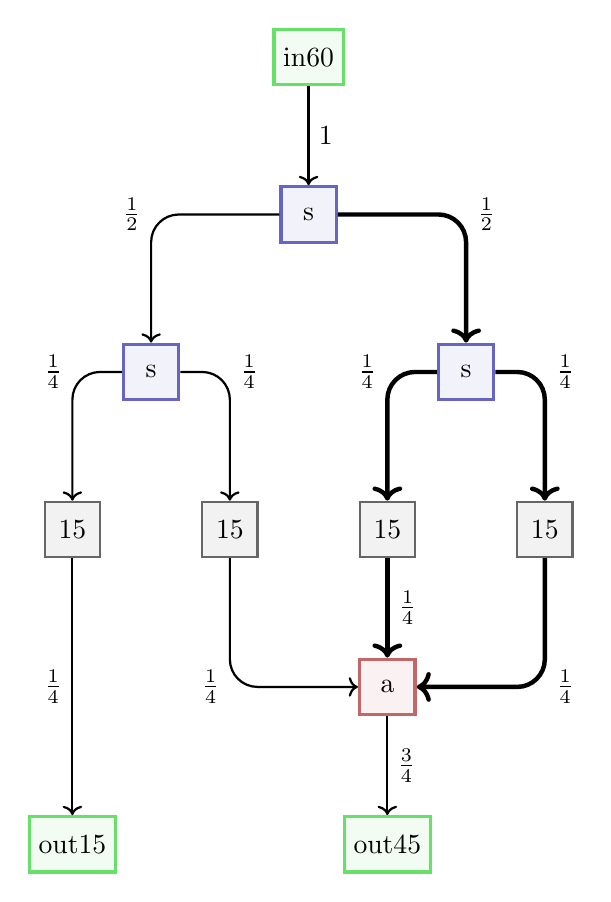
\begin{tikzpicture}[
		s/.style = {rectangle, draw=blue!60, fill=blue!5, very thick, minimum size=20},
		a/.style = {rectangle, draw=red!60, fill=red!5, very thick, minimum size=20},
		o/.style = {rectangle, draw=green!60, fill=green!5, very thick, minimum size=20},
		t/.style = {rectangle, draw=black!60, fill=black!5, thick, minimum size=20},
		r/.style = {->, thick, rounded corners=10pt},
		!/.style = {->, ultra thick, rounded corners=10pt}
		]
		
		%Nodes
		\node[o]	(in)	at	(0, 4)		{in \newline 60};
		\node[s]	(s1)	at	(0, 2)		{s};
		\node[s]	(s2)	at	(-2, 0)		{s};
		\node[s]	(s3)	at	(2, 0)		{s};
		\node[t]	(t1)	at	(-3, -2)	{15};
		\node[t]	(t2)	at	(-1, -2)	{15};
		\node[t]	(t3)	at	(1, -2)		{15};
		\node[t]	(t4)	at	(3, -2)		{15};
		\node[a]	(a)		at	(1, -4)		{a};
		\node[o]	(out1)	at	(-3, -6)	{out \newline 15};
		\node[o]	(out2)	at	(1, -6)		{out \newline 45};
		
		%Lines
		\draw[r]	(in.south) 	to	node[right]	{$1$}			(s1.north);
		\draw[r]	(s1.west)	-|	node[left]	{$\frac{1}{2}$}	(s2.north);
		\draw[!]	(s1.east)	-|	node[right]	{$\frac{1}{2}$}	(s3.north);
		\draw[r]	(s2.west)	-|	node[left]	{$\frac{1}{4}$}	(t1.north);
		\draw[r]	(s2.east)	-|	node[right]	{$\frac{1}{4}$}	(t2.north);
		\draw[!]	(s3.west)	-|	node[left]	{$\frac{1}{4}$}	(t3.north);
		\draw[!]	(s3.east)	-|	node[right]	{$\frac{1}{4}$}	(t4.north);
		\draw[r]	(t1.south)	to	node[left]	{$\frac{1}{4}$}	(out1.north);
		\draw[r]	(t2.south)	|-	node[left]	{$\frac{1}{4}$}	(a.west);
		\draw[!]	(t3.south)	to	node[right]	{$\frac{1}{4}$}	(a.north);
		\draw[!]	(t4.south)	|-	node[right]	{$\frac{1}{4}$}	(a.east);
		\draw[r]	(a.south)	to	node[right]	{$\frac{3}{4}$}	(out2.north);
	\end{tikzpicture}
	
	\
	
	$$\text{Рис. 1}$$
\end{minipage}
\hspace{37.5pt}
\begin{minipage}{0.1\textwidth}
	$$\equiv$$
\end{minipage}
\hspace{12.5pt}
\begin{minipage}{0.2\textwidth}
	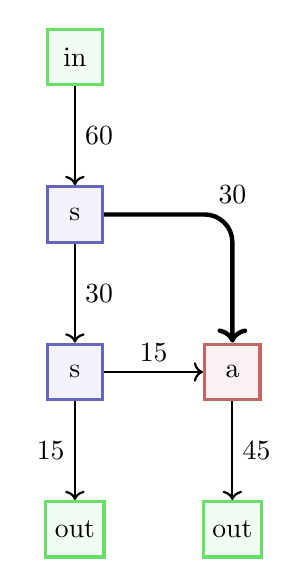
\begin{tikzpicture}[
		s/.style = {rectangle, draw=blue!60, fill=blue!5, very thick, minimum size=20},
		a/.style = {rectangle, draw=red!60, fill=red!5, very thick, minimum size=20},
		o/.style = {rectangle, draw=green!60, fill=green!5, very thick, minimum size=20},
		r/.style = {->, thick, rounded corners=10pt},
		!/.style = {->, ultra thick, rounded corners=10pt}
		]
		
		%Nodes
		\node[o]	(in)	at	(0, 4)	{in};
		\node[s]	(s1)	at	(0, 2)	{s};
		\node[s]	(s2)	at	(0, 0)	{s};
		\node[a]	(a)		at	(2, 0)	{a};
		\node[o]	(out1)	at	(0, -2)	{out};
		\node[o]	(out2)	at	(2, -2)	{out};
		
		%Lines
		\draw[r]	(in.south) 	to	node[right]	{$60$}	(s1.north);
		\draw[r]	(s1.south)	to	node[right]	{$30$}	(s2.north);
		\draw[!]	(s1.east)	-|	node[above]	{$30$}	(a.north);
		\draw[r]	(s2.east)	to	node[above]	{$15$}	(a.west);
		\draw[r]	(s2.south)	to	node[left]	{$15$}	(out1.north);
		\draw[r]	(a.south)	to	node[right]	{$45$}	(out2.north);
	\end{tikzpicture}
	
	\
	
	$$\text{Рис. 2}$$
\end{minipage}

\vspace{0.3in}

Заметим, что на рис. 1 имеется \textbf{область}, в которой разделение безсмысленно, ведь отделённые друг от друга конвейеры затем вновь соединяются. Тогда можно убрать данный разделитель, оставив целиковый \textbf{конвейер}.




\vspace{0.3in}

Для рассмотрения алгебраической картины данной задачи, нам потребуется ввести обозначение: за ответвления в стороны, с припиской в виде числа будем обозначать, что столько-то конвейеров уходят в новую ветку схемы:


\begin{minipage}{0.2\textwidth}
	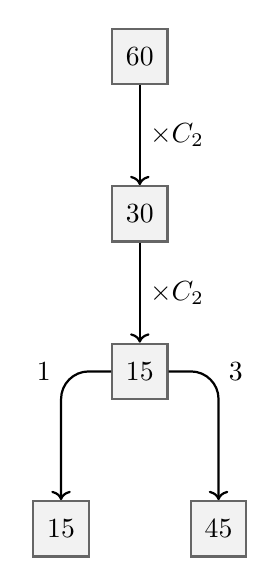
\begin{tikzpicture}[
		t/.style = {rectangle, draw=black!60, fill=black!5, thick, minimum size=20},
		r/.style = {->, thick, rounded corners=10pt}
		]
		
		%Nodes
		\node[t]	(1)		at	(0, 4)		{$60$};
		\node[t]	(2)		at	(0, 2)		{$30$};
		\node[t]	(e)		at	(0, 0)		{$15$};
		\node[t]	(out1)	at	(-1, -2)	{$15$};
		\node[t]	(out2)	at	(1, -2)		{$45$};
		
		%Lines
		\draw[r]	(1.south)	to	node[right]	{$\times C_2$}	(2.north);
		\draw[r]	(2.south)	to	node[right]	{$\times C_2$}	(e.north);
		\draw[r]	(e.west)	-|	node[left]	{$1$}			(out1.north);
		\draw[r]	(e.east)	-|	node[right]	{$3$}			(out2.north);
	\end{tikzpicture}
\end{minipage}
\begin{minipage}{0.1\textwidth}
	$$\equiv$$
\end{minipage}
\begin{minipage}{0.2\textwidth}
	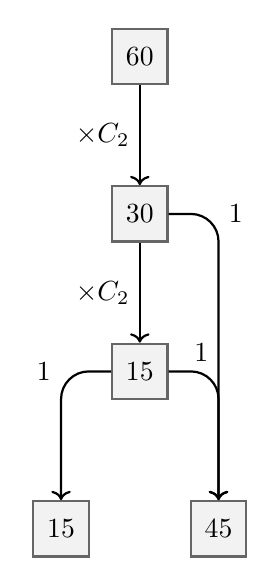
\begin{tikzpicture}[
		t/.style = {rectangle, draw=black!60, fill=black!5, thick, minimum size=20},
		r/.style = {->, thick, rounded corners=10pt}
		]
		
		%Nodes
		\node[t]	(1)		at	(0, 4)		{$60$};
		\node[t]	(2)		at	(0, 2)		{$30$};
		\node[t]	(4)		at	(0, 0)		{$15$};
		\node[t]	(out1)	at	(-1, -2)	{$15$};
		\node[t]	(out2)	at	(1, -2)		{$45$};
		
		%Lines
		\draw[r]	(1.south)	to	node[left]	{$\times C_2$}	(2.north);
		\draw[r]	(2.south)	to	node[left]	{$\times C_2$}	(4.north);
		\draw[r]	(4.west)	-|	node[left]	{$1$}			(out1.north);
		\draw[r]	(2.east)	-|	node[right]	{$1$}			(out2.north);
		\draw[r]	(4.east)	-|	node[above left]	{$1$}		(out2.north);
	\end{tikzpicture}
\end{minipage}

\vspace{0.3in}

Как видим, при упрощении схемы мы получим, что число конвейеров, идущих на соединение не превышает период циклической группы последнего сплиттера: это будет важным моментом, когда мы будем писать программное решение к задаче.
















\vspace{0.5in}

\subsection{Рекурсия}

\noindent От конвейера в 60 требуется отделить 12

\vspace{0.1in}

$\frac{12}{60} = \frac{1}{5} = \frac{1}{6} - \frac{1}{6} = \frac{1}{2}\cdot\frac{1}{3} - \frac{1}{2}\cdot\frac{1}{3} \ , \ \frac{60-12}{60} = \frac{48}{60} = \frac{4}{5} = \frac{4}{6} - \frac{1}{6} = \frac{2}{3} - \frac{1}{2}\cdot\frac{1}{3}$

\vspace{0.5in}

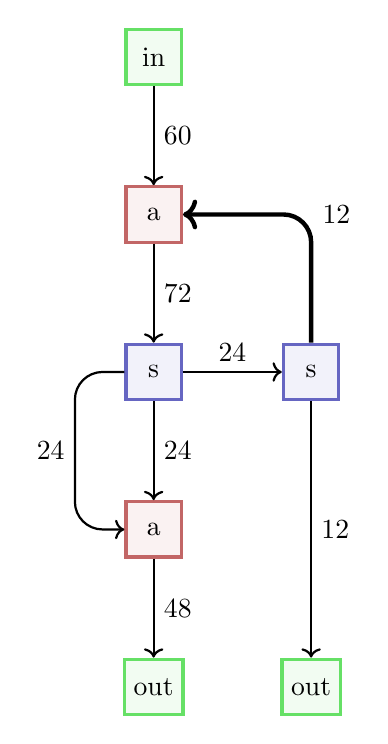
\begin{tikzpicture}[
	s/.style = {rectangle, draw=blue!60, fill=blue!5, very thick, minimum size=20},
	a/.style = {rectangle, draw=red!60, fill=red!5, very thick, minimum size=20},
	o/.style = {rectangle, draw=green!60, fill=green!5, very thick, minimum size=20},
	r/.style = {->, thick, rounded corners=10pt},
	!/.style = {->, ultra thick, rounded corners=10pt}
	]
	
	%Nodes
	\node[o]	(in)	at	(0, 4)	{in};
	\node[a]	(a1)	at	(0, 2)	{a};
	\node[s]	(s1)	at	(0, 0)	{s};
	\node[s]	(s2)	at	(2, 0)	{s};
	\node[a]	(a2)	at	(0, -2)	{a};
	\node[o]	(out1)	at	(0, -4)	{out};
	\node[o]	(out2)	at	(2, -4)	{out};
	
	%Lines
	\draw[r]	(in.south) 	to			node[right]	{$60$}	(a1.north);
	\draw[r]	(a1.south)	to			node[right]	{$72$}	(s1.north);
	\draw[r]	(s1.east)	to			node[above]	{$24$}	(s2.west);
	\draw[!]	(s2.north)	|-			node[right]	{$12$}	(a1.east);
	\draw[r]	(s1.west)	-| (-1, -1) node[left]	{$24$} |- (a2.west);
	\draw[r]	(s1.south)	to			node[right]	{$24$}	(a2.north);
	\draw[r]	(a2.south)	to			node[right]	{$48$}	(out1.north);
	\draw[r]	(s2.south)	to			node[right]	{$12$}	(out2.north);
\end{tikzpicture}

\vspace{0.3in}

% После соединителя представленна схема отделения $\frac16$, которая возвращается себе в зад. На вход всей системе поступает 60 рес/мин, тогда если предположить, что на один круг по этой схеме уходит ровно минута -- то к началу успеют прийти $\frac{60}{6}=10$ ресурсов, и после соединителя пойдёт уже 70 рес/мин. Ещё минуту спустя, на начало прийдёт уже $\frac{70}{6} \approx 11.667$ рес/мин, и после разделителя пойдёт 71.667 рес/мин. Спустя бесконечно долгое время, на участке после разделителя стабилизируется значение в 72 рес/мин. Наконец, отделив от 72, $\frac16$ -- получим требуемые 12, и на остаток 48.

Пускай, в систему импульсами подаётся по одному ресурсу раз в некоторое время%
\footnote{Такая аппроксимация возможна в связи с тем, что конвейер имеет большую скорость, и ресурсы внутри системы друг с другом не взаимодействуют},
тогда внутри делителя на 6 у каждого ресурса будет 6 различных выходов. Положим, первые 5 ресурсов ушли на свои 5 выходов, и как-то распределились в дальнейшей части конструкции. Тогда они поменяли данные, хранящиеся в памяти делителей таким образом, что 6-ой ресурс может уйти только на 6-ой выход. Но этот выход возвращён в начало системы, и тогда 6-ой ресурс становится 1-ым, так как все настройки делителей сбросились%
\footnote{Данная система является примером группы $C_2 \times C_3 = C_6$, в которой 6-ой элемент является и 0-ым}.
Таким образом, данный ресурс снова уходит на один из 5-ти допустимых выходов. Притом получается так, что порядок выходов одинаков, так что данная система является равносильной делителю на 5.



\vspace{0.3in}

\noindent Рассмотрим же теперь алгебраическую картину данной задачи:

\vspace{0.3in}


\begin{minipage}{0.2\textwidth}
	\begin{tikzpicture}[
		t/.style = {rectangle, draw=black!60, fill=black!5, thick, minimum size=20},
		r/.style = {->, thick, rounded corners=10pt}
		]
		
		%Nodes
		\node[t]	(1)		at	(0, 4)		{$60$};
		\node[t]	(3)		at	(0, 2)		{$20$};
		\node[t]	(6)		at	(0, 0)		{$10$};
		\node[t]	(5)		at	(0, -2)		{$12$};
		\node[t]	(out1)	at	(-1, -4)	{$12$};
		\node[t]	(out2)	at	(1, -4)		{$48$};
		
		%Lines
		\draw[r]	(1.south)	to	node[right]	{$\times C_3$}	(2.north);
		\draw[r]	(3.south)	to	node[right]	{$\times C_2$}	(6.north);
		\draw[r]	(6.south)	to	node[right]	{$- \frac{1}{6}$}	(5.north);
		\draw[r]	(5.west)	-|	node[left]	{$1$}			(out1.north);
		\draw[r]	(5.east)	-|	node[right]	{$4$}			(out2.north);
	\end{tikzpicture}
\end{minipage}
\begin{minipage}{0.1\textwidth}
	$$\equiv$$
\end{minipage}
\begin{minipage}{0.2\textwidth}
	\begin{tikzpicture}[
		t/.style = {rectangle, draw=black!60, fill=black!5, thick, minimum size=20},
		r/.style = {->, thick, rounded corners=10pt}
		]
		
		%Nodes
		\node[t]	(1)		at	(0, 4)		{$60$};
		\node[t]	(3)		at	(0, 2)		{$20$};
		\node[t]	(6)		at	(0, 0)		{$10$};
		\node[t]	(5)		at	(0, -2)		{$12$};
		\node[t]	(out2)	at	(1, -2)		{$48$};
		
		%Lines
		\draw[r]	(1.south)	to	node[right]	{$\times C_3$}	(2.north);
		\draw[r]	(3.south)	to	node[left]	{$\times C_2$}	(6.north);
		\draw[r]	(6.south)	to	node[left]	{$- \frac{1}{6}$}	(5.north);
		\draw[r]	(3.east)	-|	node[right]	{$2$}			(out2.north);
	\end{tikzpicture}
\end{minipage}

\vspace{0.3in}

Забавно, что граф можнт разбиваться на несколько, казалось бы независимых ветвей, но применив операцию возврата в одной ветви -- автоматически меняется значение и во всех других ветвях. 












\vspace{0.5in}

\subsection{Вариативность}

\noindent От конвейера в 60 требуется отделить 6. Рассмотрим все (сокращённые) варианты такой схемы:

$\frac{6}{60} = \frac{1}{10} = \frac{1}{12} - \frac{2}{12} = \frac{1}{2}\cdot\frac{1}{2}\cdot\frac{1}{3} - \frac{1}{6}$

\vspace{0.5in}



\begin{minipage}{0.2\textwidth}
	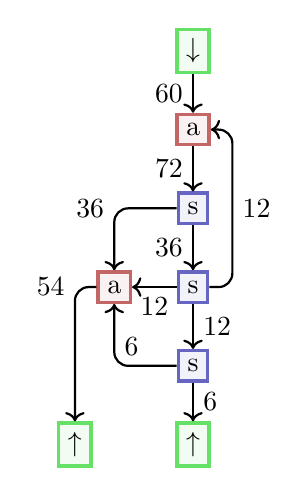
\begin{tikzpicture}[
		s/.style = {rectangle, draw=blue!60,	fill=blue!5,	very thick, minimum size=10},
		a/.style = {rectangle, draw=red!60,		fill=red!5,		very thick, minimum size=10},
		o/.style = {rectangle, draw=green!60,	fill=green!5,	very thick, minimum size=10},
		r/.style = {->, thick, rounded corners=5pt}
		]
		
		%Nodes
		\node[o]	(in)	at	(0, 3)		{$\downarrow$};
		\node[a]	(a1)	at	(0, 2)		{a};
		\node[s]	(s1)	at	(0, 1)		{s};
		\node[s]	(s2)	at	(0, 0)		{s};
		\node[s]	(s3)	at	(0, -1)		{s};
		\node[a]	(a2)	at	(-1, 0)		{a};
		\node[o]	(out1)	at	(-1.5, -2)		{$\uparrow$};
		\node[o]	(out2)	at	(0, -2)	{$\uparrow$};
		
		%Lines
		\draw[r]	(in.south)	to	node[left]	{$60$}	(a1.north);
		\draw[r]	(a1.south)	to	node[left]	{$72$}	(s1.north);
		\draw[r]	(s1.south)	to	node[left]	{$36$}	(s2.north);
		\draw[r]	(s2.east)	-| (0.5, 1) node[right] {$12$} |- (a1.east);
		\draw[r]	(s2.south)	to	node[right]	{$12$}	(s3.north);
		\draw[r]	(s1.west)	-|	node[left]	{$36$}	(a2.north);
		\draw[r]	(s2.west)	to	node[below]	{$12$}	(a2.east);
		\draw[r]	(s3.west)	-|	node[above right]	{$6$}	(a2.south);
		\draw[r]	(a2.west)	-|	node[left]	{$54$}	(out1.north);
		\draw[r]	(s3.south)	to	node[right]	{$6$}	(out2.north);
	\end{tikzpicture}
	
	\
	
	$$\text{Рис. 1}$$
\end{minipage}
\hspace{15pt}
\begin{minipage}{0.2\textwidth}
	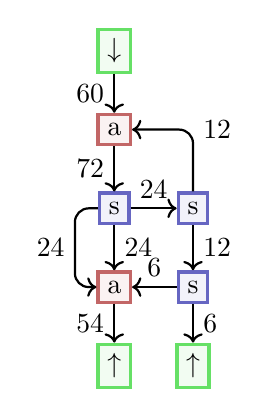
\begin{tikzpicture}[
		s/.style = {rectangle, draw=blue!60,	fill=blue!5,	very thick, minimum size=10},
		a/.style = {rectangle, draw=red!60,		fill=red!5,		very thick, minimum size=10},
		o/.style = {rectangle, draw=green!60,	fill=green!5,	very thick, minimum size=10},
		r/.style = {->, thick, rounded corners=5pt}
		]
		
		%Nodes
		\node[o]	(in)	at	(0, 3)	{$\downarrow$};
		\node[a]	(a1)	at	(0, 2)	{a};
		\node[s]	(s1)	at	(0, 1)	{s};
		\node[a]	(a2)	at	(0, 0)	{a};
		\node[s]	(s2)	at	(1, 1)	{s};
		\node[s]	(s3)	at	(1, 0)	{s};
		\node[o]	(out1)	at	(0, -1)	{$\uparrow$};
		\node[o]	(out2)	at	(1, -1)	{$\uparrow$};
		
		%Lines
		\draw[r]	(in.south)	to	node[left]	{$60$}	(a1.north);
		\draw[r]	(a1.south)	to	node[left]	{$72$}	(s1.north);
		\draw[r]	(s1.east)	to	node[above]	{$24$}	(s2.west);
		\draw[r]	(s2.north)	|-	node[right]	{$12$}	(a1.east);
		\draw[r]	(s2.south)	to	node[right]	{$12$}	(s3.north);
		\draw[r]	(s1.south)	to	node[right]	{$24$}	(a2.north);
		\draw[r]	(s1.west)	-| (-0.5, 0.5) node[left] {$24$} |- (a2.west);
		\draw[r]	(s3.west)	to	node[above]	{$6$}	(a2.east);
		\draw[r]	(a2.south)	to	node[left]	{$54$}	(out1.north);
		\draw[r]	(s3.south)	to	node[right]	{$6$}	(out2.north);
	\end{tikzpicture}
	
	\
	
	$$\text{Рис. 2}$$
\end{minipage}
\hspace{15pt}
\begin{minipage}{0.2\textwidth}
	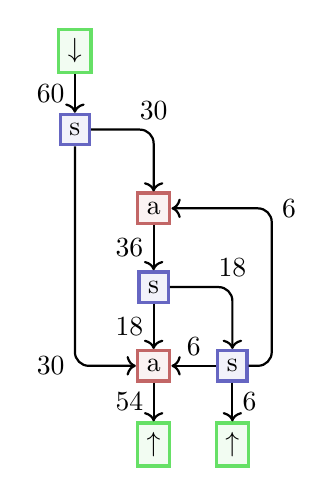
\begin{tikzpicture}[
		s/.style = {rectangle, draw=blue!60,	fill=blue!5,	very thick, minimum size=10},
		a/.style = {rectangle, draw=red!60,		fill=red!5,		very thick, minimum size=10},
		o/.style = {rectangle, draw=green!60,	fill=green!5,	very thick, minimum size=10},
		r/.style = {->, thick, rounded corners=5pt}
		]
		
		%Nodes
		\node[o]	(in)	at	(0, 3)		{$\downarrow$};
		\node[s]	(s1)	at	(0, 2)		{s};
		\node[a] 	(a1)	at	(1, 1)		{a};
		\node[s]	(s2)	at	(1, 0)		{s};
		\node[s]	(s3)	at	(2, -1)		{s};
		\node[a]	(a2)	at	(1, -1)		{a};
		\node[o]	(out1)	at	(1, -2)		{$\uparrow$};
		\node[o]	(out2)	at	(2, -2)		{$\uparrow$};
		
		%Lines
		\draw[r]	(in.south)	to	node[left]	{$60$}	(s1.north);
		\draw[r]	(s1.east)	-|	node[above]	{$30$}	(a1.north);
		\draw[r]	(a1.south)	to	node[left]	{$36$}	(s2.north);
		\draw[r]	(s2.east)	-|	node[above]	{$18$}	(s3.north);
		\draw[r]	(s1.south)	|-	node[left]	{$30$}	(a2.west);
		\draw[r]	(s2.south)	to	node[left]	{$18$}	(a2.north);
		\draw[r]	(s3.west)	to	node[above]	{$6$}	(a2.east);
		\draw[r]	(a2.south)	to	node[left]	{$54$}	(out1.north);
		\draw[r]	(s3.south)	to	node[right]	{$6$}	(out2.north);
		\draw[r]	(s3.east)	to (2.5, -1) |- node[right] {$6$} (a1.east);
	\end{tikzpicture}
	
	\
	
	$$\text{Рис. 3}$$
\end{minipage}
\hspace{15pt}
\begin{minipage}{0.2\textwidth}
	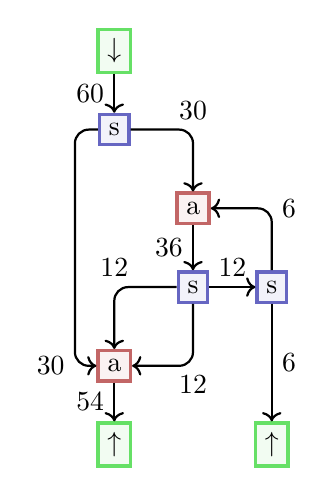
\begin{tikzpicture}[
		s/.style = {rectangle, draw=blue!60,	fill=blue!5,	very thick, minimum size=10},
		a/.style = {rectangle, draw=red!60,		fill=red!5,		very thick, minimum size=10},
		o/.style = {rectangle, draw=green!60,	fill=green!5,	very thick, minimum size=10},
		r/.style = {->, thick, rounded corners=5pt}
		]
		
		%Nodes
		\node[o]	(in)	at	(0, 3)		{$\downarrow$};
		\node[s]	(s1)	at	(0, 2)		{s};
		\node[a] 	(a1)	at	(1, 1)		{a};
		\node[s]	(s2)	at	(1, 0)		{s};
		\node[s]	(s3)	at	(2, 0)		{s};
		\node[a]	(a2)	at	(0, -1)		{a};
		\node[o]	(out1)	at	(0, -2)		{$\uparrow$};
		\node[o]	(out2)	at	(2, -2)		{$\uparrow$};
		
		%Lines
		\draw[r]	(in.south)	to	node[left]	{$60$}	(s1.north);
		\draw[r]	(s1.east)	-|	node[above]	{$30$}	(a1.north);
		\draw[r]	(a1.south)	to	node[left]	{$36$}	(s2.north);
		\draw[r]	(s2.east)	to	node[above]	{$12$}	(s3.west);
		\draw[r]	(s1.west)	to (-0.5, 2) |-	node[left]	{$30$}	(a2.west);
		\draw[r]	(s2.south)	|-	node[below]	{$12$}	(a2.east);
		\draw[r]	(s2.west)	-|	node[above]	{$12$}	(a2.north);
		\draw[r]	(a2.south)	to	node[left]	{$54$}	(out1.north);
		\draw[r]	(s3.south)	to	node[right]	{$6$}	(out2.north);
		\draw[r]	(s3.north)	|- 	node[right] {$6$}	(a1.east);
	\end{tikzpicture}
	
	\
	
	$$\text{Рис. 4}$$
\end{minipage}



\vspace{0.3in}

Заметим, что в во всех схемах, являющихся сокращёнными вариациями реализации одного и того же решения, число соединителей и разъединителей -- инвариантно относительно топологии графа. Притом сохраняется ещё и число входов/выходов конкретного узла, а так же сохраняются подструктуры по типу циклов:





\vspace{0.5in}

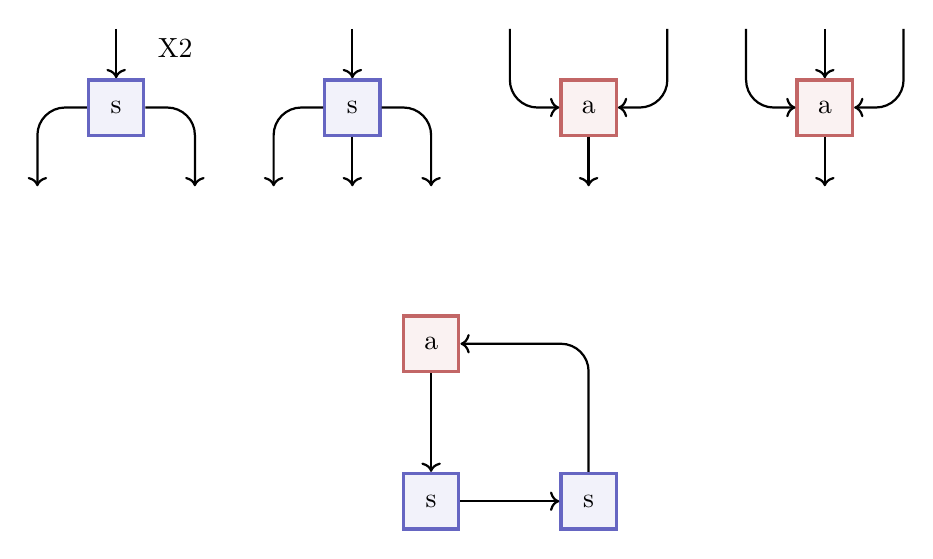
\begin{tikzpicture}[
		s/.style = {rectangle, draw=blue!60,	fill=blue!5,	very thick, minimum size=20},
		a/.style = {rectangle, draw=red!60,		fill=red!5,		very thick, minimum size=20},
		o/.style = {rectangle, draw=green!60,	fill=green!5,	very thick, minimum size=20},
		r/.style = {->, thick, rounded corners=10pt}
		]
		
		\node[s]	(s1)	at	(-6, 0)		{s};
		\draw[r]	(-6, 1)	to	(s1.north);
		\draw[r]	(s1.west)	-|	(-7, -1);
		\draw[r]	(s1.east)	-|	(-5, -1);
		\node (x) at (-5.25, 0.75) {X2};
		
		\node[s]	(s2)	at	(-3, 0)		{s};
		\draw[r]	(-3, 1)		to	(s2.north);
		\draw[r]	(s2.west)	-|	(-4, -1);
		\draw[r]	(s2.east)	-|	(-2, -1);
		\draw[r]	(s2.south)	to	(-3, -1);
		
		\node[a]	(a1)	at	(0, 0)		{a};
		\draw[r]	(-1, 1)		|-	(a1.west);
		\draw[r]	(1, 1)		|-	(a1.east);
		\draw[r]	(a1.south)	to	(0, -1);
		
		\node[a]	(a2)	at	(3, 0)		{a};
		\draw[r]	(2, 1)		|-	(a2.west);
		\draw[r]	(4, 1)		|-	(a2.east);
		\draw[r]	(3, 1)		to	(a2.north);
		\draw[r]	(a2.south)	to	(3, -1);
		
		
		
		\node[a]	(a3)	at	(-2, -3)	{a};
		\node[s]	(s4)	at	(-2, -5)	{s};
		\node[s]	(s5)	at	(0, -5)		{s};	
		\draw[r]	(a3.south)	to	(s4.north);
		\draw[r]	(s4.east)	to	(s5.west);
		\draw[r]	(s5.north)	|-	(a3.east);		
\end{tikzpicture}



\vspace{0.5in}

Так же важно помнить, что это всё было только одно решерние: $s = 12$, а ведь можно было взять первые пару ближайших стандартных чисел $(12, 16, 18, \ldots)$, или стандартные числа, являющиеся чисто степенями $(16, 32, 27, \ldots)$. Так же в решении можно было использоавть нетривиальные разложения по типу: $\frac56 = \frac12 + \frac13$



\vspace{0.3in}

















\vspace{0.5in}

\subsection{Большие схемы}

\noindent Рассмотрим схему побольше: отделить $\frac17$, $\frac15$ и $\frac13$ одновременно от одного конвейера.

$\text{lcm}(3, 5, 7) = 105$

\begin{align*}
	&\frac{1}{7} = \frac{15}{105} = \frac{15}{2^2 3^3} - \frac{3}{108} = \frac{5}{36} - \frac{1}{36} = \frac{1}{36} + \frac{1}{9} - \frac{1}{36} \\
	&\frac{1}{5} = \frac{21}{105} = \frac{21}{2^2 3^3} - \frac{3}{108} = \frac{7}{36} - \frac{1}{36} = \frac{1}{36} + \frac{1}{6} - \frac{1}{36} \\
	&\frac{1}{3} = \frac{35}{105} = \frac{35}{2^2 3^3} - \frac{3}{108} = \frac{1}{36} + \frac{2}{27} + \frac{2}{9} - \frac{1}{36}
\end{align*}

Остаток: $\frac{34}{105}$






\vspace{0.5in}


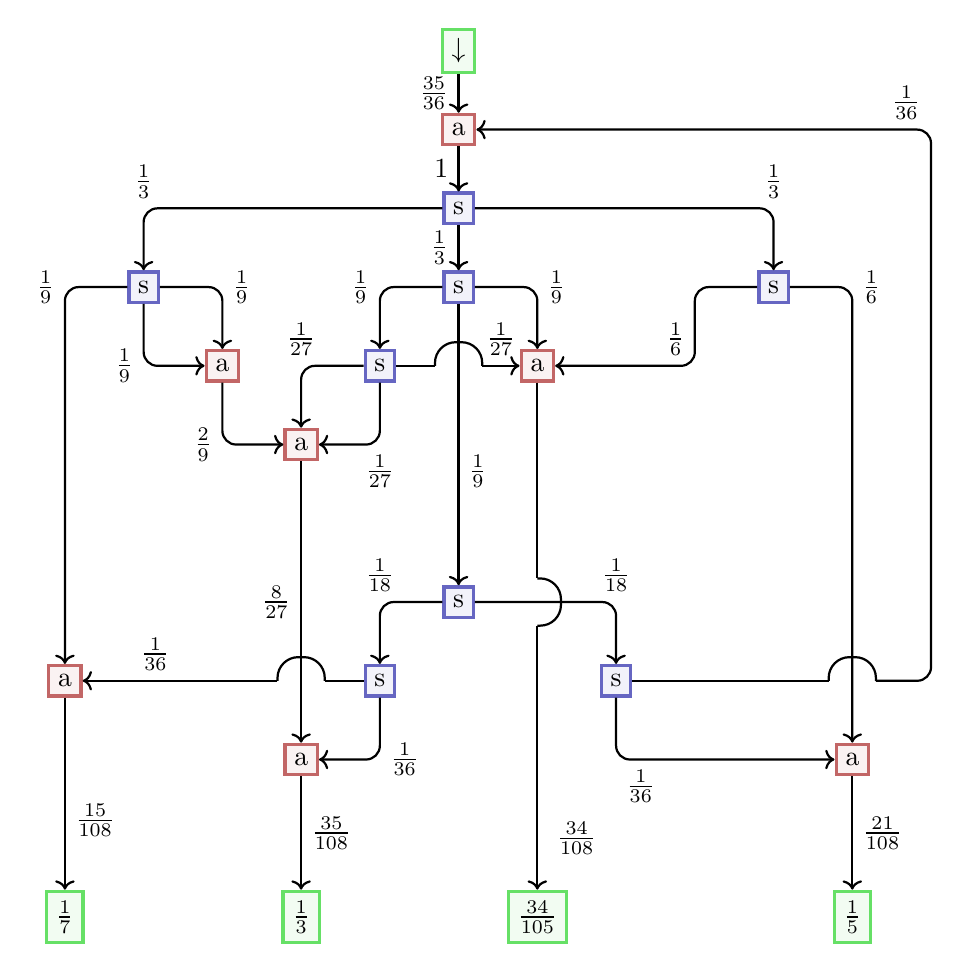
\begin{tikzpicture}[
	s/.style = {rectangle, draw=blue!60,	fill=blue!5,	very thick, minimum size=10},
	a/.style = {rectangle, draw=red!60,		fill=red!5,		very thick, minimum size=10},
	o/.style = {rectangle, draw=green!60,	fill=green!5,	very thick, minimum size=10},
	r/.style = {->, thick, rounded corners=5pt}
	]
	
	%Nodes
	\node[o]	(in)	at	(0, 5)		{$\downarrow$};
	\node[a]	(a1)	at	(0, 4)		{a};
	\node[s]	(s1)	at	(0, 3)		{s};
	
	\node[s]	(s2-l)	at	(-4, 2)		{s};
	\node[s]	(s2-c)	at	(0, 2)		{s};
	\node[s]	(s2-r)	at	(4, 2)		{s};
	\node[a]	(a2-l)	at	(-3, 1)		{a};
	\node[a]	(a2-c)	at	(-2, 0)		{a};
	\node[s]	(s2-2)	at	(-1, 1)		{s};
	\node[a]	(a2-r)	at	(1, 1)		{a};
	
	\node[s]	(s3)	at	(0, -2)		{s};
	\node[s]	(s4-l)	at	(-1, -3)	{s};
	\node[s]	(s4-r)	at	(2, -3)		{s};
	\node[a]	(a3-l)	at	(-5, -3)	{a};
	\node[a]	(a3-c)	at	(-2, -4)	{a};
	\node[a]	(a3-r)	at	(5, -4)		{a};
	
	\node[o]	(out1)	at	(-5, -6)	{$\frac{1}{7}$};
	\node[o]	(out2)	at	(-2, -6)	{$\frac{1}{3}$};
	\node[o]	(out3)	at	(1, -6)		{$\frac{34}{105}$};
	\node[o]	(out4)	at	(5, -6)		{$\frac{1}{5}$};
	
	
	
	%Lines
	\draw[r]	(in.south)		to	node[left]			{$\frac{35}{36}$}	(a1.north);
	\draw[r]	(a1.south)		to	node[left]			{$1$}				(s1.north);
	\draw[r]	(s1.west)		-|	node[above]			{$\frac13$}			(s2-l.north);
	\draw[r]	(s1.south)		to	node[left]			{$\frac13$}			(s2-c.north);
	\draw[r]	(s1.east)		-|	node[above]			{$\frac13$}			(s2-r.north);
	
	\draw[r]	(s2-l.south)	|-	node[left]			{$\frac19$}			(a2-l.west);
	\draw[r]	(s2-l.east)		-|	node[right]			{$\frac19$}			(a2-l.north);
	\draw[r]	(s2-c.west)		-|	node[left]			{$\frac19$}			(s2-2.north);
	\draw[r]	(s2-2.west)		-|	node[above]			{$\frac1{27}$}		(a2-c.north);
	\draw[r]	(s2-2.south)	|-	node[below]			{$\frac1{27}$}		(a2-c.east);
	\draw[r]	(a2-l.south)	|-	node[left]			{$\frac29$}			(a2-c.west);
	\draw[r]	(s2-c.east)		-|	node[right]			{$\frac19$}			(a2-r.north);
	
	\draw[r] (s2-r.west) to (3, 2) |- node[above left] {$\frac16$} (a2-r.east);
	\draw[thick] (s2-2.east) -- (-0.3, 1);
	\draw[thick, rounded corners=7.5pt] (-0.3, 1) |- (0, 1.3);
	\draw[thick, rounded corners=7.5pt] (0, 1.3) -| (0.3, 1);
	\draw[r] (0.3, 1) to node[above] {$\frac{1}{27}$} (a2-r.west);
	
	\draw[r]	(s2-c.south)	to	node[below right]	{$\frac{1}{9}$}		(s3.north);
	\draw[r]	(s3.west)		-|	node[above]			{$\frac{1}{18}$}	(s4-l.north);
	\draw[r]	(s3.east)		-|	node[above]			{$\frac{1}{18}$}	(s4-r.north);
	\draw[r]	(s4-l.south)	|-	node[right]			{$\frac{1}{36}$}	(a3-c.east);
	\draw[r]	(a2-c.south)	to	node[left]			{$\frac{8}{27}$}	(a3-c.north);
	\draw[r]	(s4-r.south)	|-	node[below right]	{$\frac{1}{36}$}	(a3-r.west);
	\draw[r]	(s2-r.east)		-|	node[right]			{$\frac16$}			(a3-r.north);
	\draw[r]	(s2-l.west)		-|	node[left]			{$\frac19$}			(a3-l.north);
	
	\draw[r]	(a3-l.south)	to	node[below right]	{$\frac{15}{108}$}		(out1.north);
	\draw[r]	(a3-c.south)	to	node[right]			{$\frac{35}{108}$}	(out2.north);
	\draw[r]	(a3-r.south)	to	node[right]			{$\frac{21}{108}$}		(out4.north);
	\node (n1) at (1.5, -5) {$\frac{34}{108}$};
	
	\draw[thick] (a2-r.south) -- (1, -1.7);
	\draw[thick, rounded corners=7.5pt] (1, -1.7) -| (1.3, -2);
	\draw[thick, rounded corners=7.5pt] (1.3, -2) |- (1, -2.3);
	\draw[r] (1, -2.3) to (out3.north);
	
	\draw[thick] (s4-r.east) -- (4.7, -3);
	\draw[thick, rounded corners=7.5pt] (4.7, -3) |- (5, -2.7);
	\draw[thick, rounded corners=7.5pt] (5, -2.7) -| (5.3, -3);
	\draw[r] (5.3, -3) to (6, -3) |- node[above left] {$\frac1{36}$} (a1.east);
	
	\draw[thick] (s4-l.west) -- (-1.7, -3);
	\draw[thick, rounded corners=7.5pt] (-1.7, -3) |- (-2, -2.7);
	\draw[thick, rounded corners=7.5pt] (-2, -2.7) -| (-2.3, -3);
	\draw[r] (-2.3, -3) to node[above left] {$\frac1{36}$} (a3-l.east);
	
	
	
\end{tikzpicture}











\vspace{0.5in}

Как мы можем заметить, на схемах побольше появляются две интересные вещи: \\ \underline{пересечеиния конвейеров}%
\footnote{Смотреть приложение \ref{appendix:a}: проблема перекрёстков (brick factory problem)}
и разная периодичность параллельных ветвей:






\vspace{0.3in}

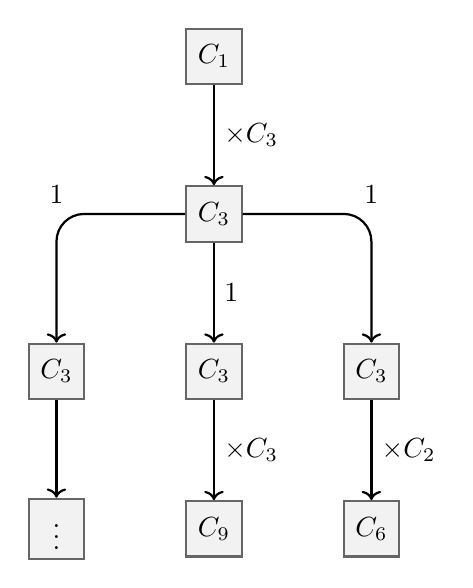
\begin{tikzpicture}[
	t/.style = {rectangle, draw=black!60, fill=black!5, thick, minimum size=20},
	r/.style = {->, thick, rounded corners=10pt}
	]
	
	%Nodes
	\node[t]	(0)		at	(0, 6)	{$C_1$};
	\node[t]	(1)		at	(0, 4)	{$C_3$};
	\node[t]	(1-l)	at	(-2, 2)	{$C_3$};
	\node[t]	(1-c)	at	(0, 2)	{$C_3$};
	\node[t]	(1-r)	at	(2, 2)	{$C_3$};
	\node[t]	(2-l)	at	(-2, 0)	{$\vdots$};
	\node[t]	(2-c)	at	(0, 0)	{$C_9$};
	\node[t]	(2-r)	at	(2, 0)	{$C_6$};
	
	
	%Lines
	\draw[r]	(0.south)	to	node[right]	{$\times C_3$}	(1.north);
	\draw[r]	(1.west)	-|	node[above]	{$1$}			(1-l.north);
	\draw[r]	(1.south)	to	node[right]	{$1$}			(1-c.north);
	\draw[r]	(1.east)	-|	node[above]	{$1$}			(1-r.north);
	\draw[r]	(1-l.south)	to								(2-l.north);
	\draw[r]	(1-c.south)	to	node[right]	{$\times C_3$}	(2-c.north);
	\draw[r]	(1-r.south)	to	node[right]	{$\times C_2$}	(2-r.north);
	
\end{tikzpicture}






\vspace{0.3in}

Как мы видим, циклические группы $C_9$ и $C_6$ находятся в дереве деления на одинаковых уровнях. Это и есть пример применения нетривиальных разложений. Давайте же тогда рассмотрим некоторые разбиения, например, дроби $\frac{34}{108}$:


\begin{align*}
	\frac{34}{108} = \frac{17}{54} = &\frac{1}{54} + \frac{8}{27} = \frac{1}{54} + \frac{2}{27} + \frac{2}{9} \\
	&\frac{1}{27} + \frac{5}{18} = \frac{1}{27} + \frac{1}{18} + \frac{2}{9} \\
	&\quad\quad\quad\quad\quad\frac{1}{27} + \frac{1}{9} + \frac{1}{6}
\end{align*}















\vspace{0.5in}

\subsection{Несколько входов}

\

Порой бывает такое, что мы имеем несколько входных конвейеров, идущих, например, с разных производств, и нам необходимо как-то перераспределить между ними ресурсы.

\

Можно пойти двумя путями: по \underline{принципу чайника}%
\footnote{Как физик заваривает чай, если чайник пустой? Наливает воду, кипитит воду, заваривает чай. \\ Как математик заваривает чай, если чайник пустой? Наливает воду, кипитит воду, заваривает чай. \\ Как физик заваривает чай, если в чайнике есть вода? Кипитит воду, заваривает чай. \\ Как математик заваривает чай, если в чайнике есть вода? Выливает воду, наливает воду, кипитит воду, заваривает чай. \\ Принцип чайника: сведи задачу к предыдущей.}
: соединить все входные конвейеры, и работать с тем, что получим; или  поиграться с отделениями в самих конвейерах. Рассматривать мы будем второй метод, так как он является обобщением первого.

\

\noindent Пример:

Входы: 4, 8, 10, 18

Выходы: 5, 8, 12, 15

\vspace{0.5in}

\begin{minipage}{0.4\textwidth}
	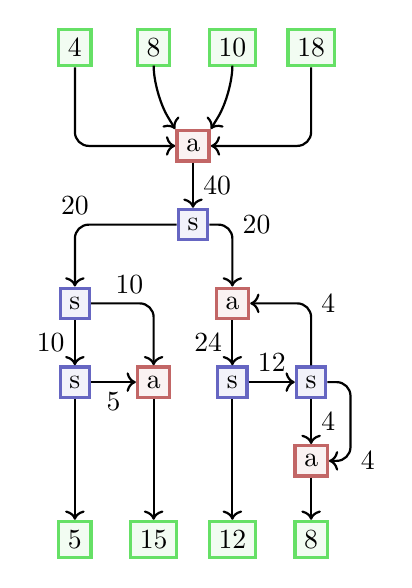
\begin{tikzpicture}[
		s/.style = {rectangle, draw=blue!60,	fill=blue!5,	very thick, minimum size=10},
		a/.style = {rectangle, draw=red!60,		fill=red!5,		very thick, minimum size=10},
		o/.style = {rectangle, draw=green!60,	fill=green!5,	very thick, minimum size=10},
		r/.style = {->, thick, rounded corners=5pt},
		b/.style = {->, thick, rounded corners=10pt}
		]
		
		% === === Nodes === ===
		\node[o]	(in1)	at	(-1, 3.25)		{$4$};	
		\node[o]	(in2)	at	(0, 3.25)		{$8$};	
		\node[o]	(in3)	at	(1, 3.25)		{$10$};	
		\node[o]	(in4)	at	(2, 3.25)		{$18$};
		\node[a]	(a0)	at	(0.5, 2)		{a};
		\node[s]	(s1)	at	(0.5, 1)		{s};
		
		\node[s]	(s2)	at	(-1, 0)			{s};
		\node[a]	(a1)	at	(1, 0)			{a};
		\node[s]	(s3-l)	at	(-1, -1)		{s};
		\node[s]	(s3-c)	at	(1, -1)			{s};
		\node[s]	(s3-r)	at	(2, -1)			{s};
		\node[a]	(a2-l)	at	(0, -1)			{a};
		\node[a]	(a2-r)	at	(2, -2)			{a};
		
		\node[o]	(out1)	at	(-1, -3)		{$5$};
		\node[o]	(out2)	at	(0, -3)			{$15$};
		\node[o]	(out3)	at	(1, -3)			{$12$};
		\node[o]	(out4)	at	(2, -3)			{$8$};
		
		
		
		% === === Lines === ===
		\draw[r]	(in1.south)		|-							(a0.west);
		\draw[r]	(in4.south)		|-							(a0.east);
		\draw[b] (in2.south) -- (0, 2.667) -- (a0.north west);
		\draw[b] (in3.south) -- (1, 2.667) -- (a0.north east);
		\draw[r]	(a0.south)		to	node[right]	{$40$}	(s1.north);
		
		\draw[r]	(s1.west)		-|	node[above]		{$20$}	(s2.north);
		\draw[r]	(s1.east)		-|	node[right]		{$20$}	(a1.north);
		\draw[r]	(s2.south)		to	node[left]		{$10$}	(s3-l.north);
		\draw[r] 	(s3-l.east) 	to 	node[below] 	{$5$} 	(a2-l.west);
		\draw[r]	(s2.east)		-|	node[above left]	{$10$}	(a2-l.north);	
		
		\draw[r]	(a1.south)		to	node[left]		{$24$}	(s3-c.north);
		\draw[r]	(s3-c.east)		to	node[above]		{$12$}	(s3-r.west);
		\draw[r]	(s3-r.north)	|-	node[right]		{$4$}	(a1.east);
		\draw[r]	(s3-r.south)	to	node[right]		{$4$}	(a2-r.north);
		\draw[r] (s3-r.east) -| (2.5, -1.5) |- node[right] {$4$} (a2-r.east);
		
		\draw[r]	(s3-l.south)	to							(out1.north);
		\draw[r]	(a2-l.south)	to							(out2.north);
		\draw[r]	(s3-c.south)	to							(out3.north);
		\draw[r]	(a2-r.south)	to							(out4.north);
		
		
	\end{tikzpicture}
\end{minipage}
\begin{minipage}{0.4\textwidth}
	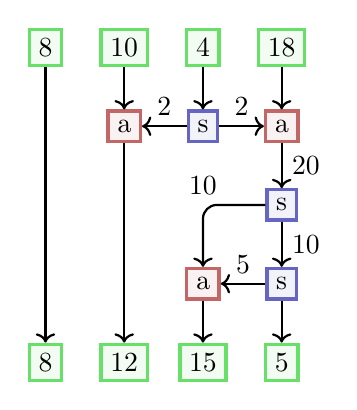
\begin{tikzpicture}[
		s/.style = {rectangle, draw=blue!60,	fill=blue!5,	very thick, minimum size=10},
		a/.style = {rectangle, draw=red!60,		fill=red!5,		very thick, minimum size=10},
		o/.style = {rectangle, draw=green!60,	fill=green!5,	very thick, minimum size=10},
		r/.style = {->, thick, rounded corners=5pt},
		b/.style = {->, thick, rounded corners=10pt}
		]
		
		% === === Nodes === ===
		\node[o]	(in1)	at	(-1, 3)		{$8$};	
		\node[o]	(in2)	at	(0, 3)		{$10$};	
		\node[o]	(in3)	at	(1, 3)		{$4$};	
		\node[o]	(in4)	at	(2, 3)		{$18$};
		
		\node[s]	(s0)	at	(1, 2)		{s};
		\node[a]	(a0-r)	at	(2, 2)		{a};
		\node[a]	(a0-l)	at	(0, 2)		{a};
		\node[s]	(s1)	at	(2, 1)		{s};
		\node[s]	(s2)	at	(2, 0)		{s};
		\node[a]	(a1)	at	(1, 0)		{a};
		
		\node[o]	(out1)	at	(-1, -1)	{$8$};	
		\node[o]	(out2)	at	(0, -1)		{$12$};	
		\node[o]	(out3)	at	(1, -1)		{$15$};	
		\node[o]	(out4)	at	(2, -1)		{$5$};
		
		
		
		% === === Lines === ===
		\draw[r] 	(in1.south)		to	(out1.north);
		\draw[r]	(in2.south)		to	(a0-l.north);
		\draw[r]	(in3.south)		to	(s0.north);
		\draw[r]	(in4.south)		to	(a0-r.north);
		\draw[r]	(a0-l.south)	to	(out2.north);
		\draw[r]	(a1.south)		to	(out3.north);
		\draw[r]	(s2.south)		to	(out4.north);
		
		\draw[r]	(s0.west)		to	node[above]	{$2$}	(a0-l.east);
		\draw[r]	(s0.east)		to	node[above]	{$2$}	(a0-r.west);
		\draw[r]	(a0-r.south)	to	node[right]	{$20$}	(s1.north);
		\draw[r]	(s1.south)		to	node[right]	{$10$}	(s2.north);
		\draw[r]	(s1.west)		-|	node[above]	{$10$}	(a1.north);
		\draw[r]	(s2.west)		to	node[above]	{$5$}	(a1.east);
		
	\end{tikzpicture}
\end{minipage}





\vspace{0.5in}

Очевидно, что вторая схема проще первой. Хотя, на самом деле, это не всегда так, и нам просто повезло. Иногда эти две схемы могут быть вообще одинаковыми (например от (10, 10, 10, 10) отделить (5, 8, 12, 15)). 

\

Однако даже так, её можно упростить: как нам уже известно, такая схема является матрицей преобразования вида:



$$
\left[
\begin{matrix}
	5 \\ 8 \\ 15 \\ 12
\end{matrix}
\right]
=
\left[
\begin{matrix}
	m_{11} & \ldots & m_{14} \\
	\vdots & \ddots & \vdots \\
	m_{41} & \ldots & m_{44}
\end{matrix}
\right]
\times
\left[
\begin{matrix}
	10 \\ 8 \\ 4 \\ 18
\end{matrix}
\right]
$$



\

\noindent И имеет решение, например:

$$
\left[
\begin{matrix}
	5 \\ 8 \\ 15 \\ 12
\end{matrix}
\right]
=
\left[
\begin{matrix}
	\frac12 & 0 & 0 & 0 \\
	0 		& 1 & 0 & 0 \\
	\frac12 & 0 & 1	& \frac13 \\
	0		& 0 & 0 & \frac23 \\
\end{matrix}
\right]
\times
\left[
\begin{matrix}
	10 \\ 8 \\ 4 \\ 18
\end{matrix}
\right]
$$






\vspace{0.5in}


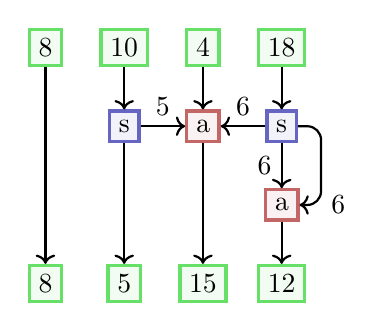
\begin{tikzpicture}[
	s/.style = {rectangle, draw=blue!60,	fill=blue!5,	very thick, minimum size=10},
	a/.style = {rectangle, draw=red!60,		fill=red!5,		very thick, minimum size=10},
	o/.style = {rectangle, draw=green!60,	fill=green!5,	very thick, minimum size=10},
	r/.style = {->, thick, rounded corners=5pt},
	b/.style = {->, thick, rounded corners=10pt}
	]
	
	% === === Nodes === ===
	\node[o]	(in1)	at	(-1, 3)	{$8$};	
	\node[o]	(in2)	at	(0, 3)	{$10$};	
	\node[o]	(in3)	at	(1, 3)	{$4$};	
	\node[o]	(in4)	at	(2, 3)	{$18$};
	
	\node[s]	(s1)	at	(0, 2)	{s};
	\node[s]	(s2)	at	(2, 2)	{s};
	\node[a]	(a1)	at	(1, 2)	{a};
	\node[a]	(a2)	at	(2, 1)	{a};
	
	\node[o]	(out1)	at	(-1, 0)	{$8$};	
	\node[o]	(out2)	at	(0, 0)	{$5$};	
	\node[o]	(out3)	at	(1, 0)	{$15$};	
	\node[o]	(out4)	at	(2, 0)	{$12$};
	
	
	
	% === === Lines === ===
	\draw[r]	(in1.south)	to	(out1.north);
	\draw[r]	(in2.south)	to	(s1.north);
	\draw[r]	(s1.south)	to	(out2.north);
	\draw[r]	(s1.east)	to	node[above]	{$5$}	(a1.west);
	\draw[r]	(in3.south)	to	(a1.north);
	\draw[r]	(in4.south)	to	(s2.north);
	\draw[r]	(s2.west)	to	node[above]	{$6$}	(a1.east);
	\draw[r]	(a1.south)	to	(out3.north);
	\draw[r]	(s2.south)	to	node[left]	{$6$}	(a2.north);
	\draw[r]	(s2.east)	-|	(2.5, 1.5)	|-	node[right]	{$6$}	(a2.east);
	\draw[r]	(a2.south)	to	(out4.north);
	
\end{tikzpicture}



\vspace{0.5in}

Таким образом, мы получили самую простую версию схемы перераспределения ресурсов между несколькими входами и выходами.






























































\vspace{1in}

\section{Решение}

\

\noindent Любую стандартную долю можно представить, как сумму некоторого количества других стандартных дробей:

$$\forall \ \frac{a}{s} \ : \ \exists \ n \in \mathbb{N}, A = \{a_i\}, S = \{s_i\} \ | \ \frac{a}{s} = \sum_{i=1}^n \frac{a_i}{s_i}$$

\

\noindent "Элементарными" назовём несократимые стандартные дроби, для которых $n=1$, т.е.: 

$\nexists \ a_i \le a \ | \ \text{gcd}(a_i, s) \ne 1$

\

\noindent Для дроби $\frac{a}{b}$ "решением" назовём%
\footnote{под "-" подразумеваем его определение через рекурсию}
$A_b^a = O_b^a - R_b$, где:


\begin{itemize}
	\item $s = s(b)$ -- ближайшее большее стандартное к $b$
	
	\item $O_b^a = O_{s}^a = \sum_{i=1}^n \frac{a_i}{s_i}$
	
	\item $R_b = O_{s}^{s-b}$
\end{itemize}

\

\noindent Тогда задача сводится к изучению получения оптимальных $S(b)$, $O_s^a$ и $R_b$.





\vspace{0.5in}

\noindent Код на C\# для реализации поиска наименьшего $s(b)$ для множества $\mathbb{T} = \{ 2, 3 \}$:

\newpage

\begin{lstlisting}[title={C\#}, language={[Sharp]C}]
public static int hig_closest(int number, int x = 0, int y = 0, int branch = 1)
{
	int answer = -1;
	int num = Convert.ToInt32(Math.Pow(2, x) * Math.Pow(3, y));
	
	if (num >= number) { answer = num; }
	else
	{
		List<int> answers = new List<int>();
		
		answers.Add(hig_closest(number, x + 1, y, 0));
		if (branch == 1) 
		{ answers.Add(hig_closest(number, x, y + 1, 1)); }
		
		answer = answers.Min();
	}
	
	return answer;
}
\end{lstlisting}



\vspace{0.5in}

\noindent Он реализует следующее дерево поиска (пример для $b=31$):

\vspace{0.35in}

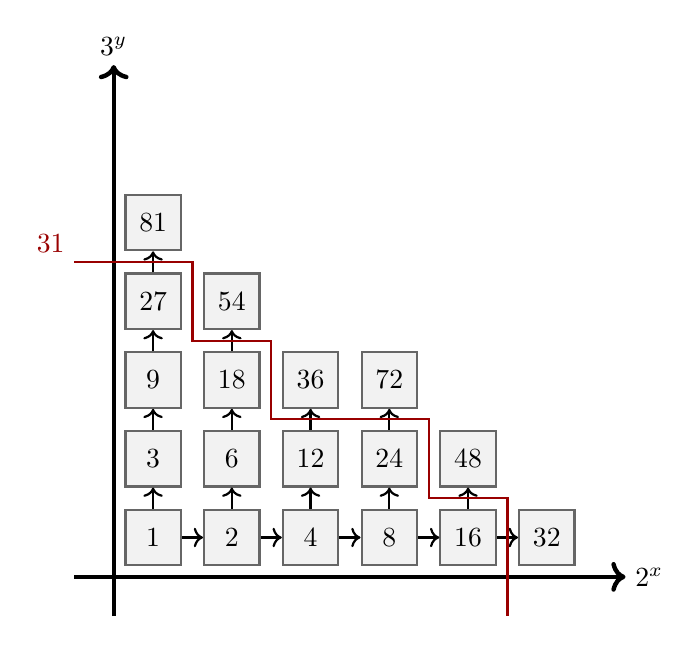
\begin{tikzpicture}[
	t/.style = {rectangle, draw=black!60, fill=black!5, thick, minimum size=20},
	r/.style = {->, thick, rounded corners=10pt}
	]
	
	% === === === Nodes === === ===
	\node[t]	(0-0)	at	(0, 0)	{1};
	\node[t]	(1-0)	at	(1, 0)	{2};
	\node[t]	(2-0)	at	(2, 0)	{4};
	\node[t]	(3-0)	at	(3, 0)	{8};
	\node[t]	(4-0)	at	(4, 0)	{16};
	\node[t]	(5-0)	at	(5, 0)	{32};
	
	\node[t]	(0-1)	at	(0, 1)	{3};
	\node[t]	(1-1)	at	(1, 1)	{6};
	\node[t]	(2-1)	at	(2, 1)	{12};
	\node[t]	(3-1)	at	(3, 1)	{24};
	\node[t]	(4-1)	at	(4, 1)	{48};
	
	\node[t]	(0-2)	at	(0, 2)	{9};
	\node[t]	(1-2)	at	(1, 2)	{18};
	\node[t]	(2-2)	at	(2, 2)	{36};
	\node[t]	(3-2)	at	(3, 2)	{72};
	
	\node[t]	(0-3)	at	(0, 3)	{27};
	\node[t]	(1-3)	at	(1, 3)	{54};
	
	\node[t]	(0-4)	at	(0, 4)	{81};
	
	
	
	% === === === Axis === === ===
	\draw[->, ultra thick]	(-1, -0.5) to (6, -0.5);
	\node[right] (x) at (6, -0.5) {$2^x$};
	\draw[->, ultra thick]	(-0.5, -1) to (-0.5, 6);
	\node[above] (y) at (-0.5, 6) {$3^y$};
	
	
	
	% === === === Lines === === ===
	\draw[r] (0-0.east) to (1-0.west);
	\draw[r] (1-0.east) to (2-0.west);
	\draw[r] (2-0.east) to (3-0.west);
	\draw[r] (3-0.east) to (4-0.west);
	\draw[r] (4-0.east) to (5-0.west);
	
	\draw[r] (0-0.north) to (0-1.south);
	\draw[r] (0-1.north) to (0-2.south);
	\draw[r] (0-2.north) to (0-3.south);
	\draw[r] (0-3.north) to (0-4.south);
	
	\draw[r] (1-0.north) to (1-1.south);
	\draw[r] (1-1.north) to (1-2.south);
	\draw[r] (1-2.north) to (1-3.south);
	
	\draw[r] (2-0.north) to (2-1.south);
	\draw[r] (2-1.north) to (2-2.south);
	
	\draw[r] (3-0.north) to (3-1.south);
	\draw[r] (3-1.north) to (3-2.south);
	
	\draw[r] (4-0.north) to (4-1.south);
	
	\draw[thick, red] (-1, 3.5) -- (0.5, 3.5) -- (0.5, 2.5) -- (1.5, 2.5) -- (1.5, 1.5) -- (3.5, 1.5) -- (3.5, 0.5) -- (4.5, 0.5) -- (4.5, -1);
	\node[above left, color=red] (31) at (-1, 3.5) {31};
	
	
\end{tikzpicture}





\vspace{0.35in}

\noindent Нетрудно модифицировать данный алгоритм для произвольных $\mathbb{T}$:

\vspace{0.2in}

\begin{lstlisting}[title={Python}, language={Python}]
def hig_closest(target, powers, branch=max(T)):
	answer = -1
	num = 1
	for i in range(0, T.len()):
		num *= T[i]**powers[i]
	
	if num >= target: return num
	
	answers = []
	for i in T:
		if i <= branch>:
			answers.append(hig_closest(target, powers.increace(i), i))
	
	answer = min(answers)
	
	return answer
\end{lstlisting}

\vspace{0.5in}




Вот нашли мы $s(b)$, а как теперь искать $O_s^a$? Ответ прост: брутфорс. Требуется перебрать все возможные способы разбиения числа $a$ на суммы всевозможных натуральных%
\footnote{Вцелом, можно и не натуральных, а просто рациональных: $\frac23 = \frac{1.5}3 + \frac{0.5}3 = \frac12 + \frac16$ -- такое разбиение вполне подойдёт для $\mathbb{T} = \{2, 6\}$. Однако, такой алгоритм слишком сложен, ведь перебирать придётся \textbf{значительно} больше вариантов}
чисел, после чего соответствующие дроби (если это возможно) мы сокрращаем дроби, а затем объединяем все дроби с одинаковыми знаменателями. Для каждого отдельного знаменателя $s_i = \prod_{j=0}^n t_j^{a_j}$ должно быть выполненно: $s_i < t_j \ \forall j$

% \
%
% !!!!! Нужно раздеять не до единиц, а только на: !!!!!
% $$a = \sum_{a_i < b \ \forall b \in \mathbb{T}} a_i$$

\

\noindent Алгоритм для поиска одного варианта разбиения:

\

\begin{lstlisting}[title={Python}, language={Python}]
def spliter(numerator, denominator):
	s = hig_closest(denominator)
	reduce_coef = gcd(s, numerator)
	numerator //= reduce_coef
	denominator = s // reduce_coef
	
	s = low_closest(numerator, denominator)
	
	if s == numerator:
		return [[numerator, denominator]]
	
	else:
		cdg1 = gcd(numerator-s, denominator)
		gcd2 = gcd(s, denominator)
		d_parts = [
			[(numerator-s)//gcd1, denominator//gcd1], 
			[s//gcd2, denominator//gdc2]
		]
	
	while 1:
		memory = []
	
		for fractions in d_parts:
			x, y = fractions[0], fractions[1]
			s = low_closest(x, y)
		
			if p != x:
				gcd1 = gcd(x-s, y)
				gcd2 = gcd(s, y)
				memory.append([(x-s)//gcd1, y//gcd1])
				memory.append([s//gcd2, y//gcd2])
			
			else: memory.append(fractions)
		
		if len(d_parts) == len(memory): break
		else: d_parts = memory[0::]
		
	return d_parts[0::]
\end{lstlisting}



\vspace{0.5in}

\noindent Полноценный алгоритм на C\# приведён в satisfactory\_conveyor\_calc.sln

































































\newpage

\section{Построение схемы}

\subsection{Степенное дерево}

\

Самый простой способ: если известно решение $A_b^a = O_b^a - R_b$ -- то можно просто в лоб реализовать дерево на $s$ листьев, $s-b$ из них вернуть в начало, $a$ соединить, и отправить на выход; а оставшиеся $b-a$ тоже соединить, и тоже на выход.

\vspace{0.5in}

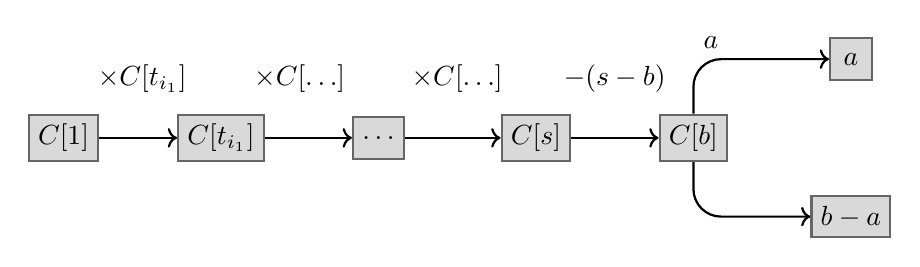
\begin{tikzpicture}[
	t/.style = {rectangle, draw=black!60, fill=black!15, thick, minimum size=15},
	r/.style = {->, thick, rounded corners=10pt}
	]
	
	%Nodes
	\node[t]	(1)		at	(-4, 0)		{$C[1]$};
	\node[t]	(2)		at	(-2, 0)		{$C[t_{i_1}]$};
	\node[t]	(e)		at	(0, 0)		{$\ldots$};
	\node[t]	(s)		at	(2, 0)		{$C[s]$};
	\node[t]	(b)		at	(4, 0)		{$C[b]$};
	
	\node		(t1)	at	(-3, 0.75)	{$\times C[t_{i_1}]$};
	\node		(t2)	at	(-1, 0.75)	{$\times C[\ldots]$};
	\node		(t3)	at	(1, 0.75)	{$\times C[\ldots]$};
	\node		(t4)	at	(3, 0.75)	{$- (s-b)$};

	\node[t]	(A)		at	(6, 1)		{$a$};
	\node[t]	(B)		at	(6, -1)		{$b-a$};
	
	
	
	%Lines
	\draw[r]	(1.east)	to	(2.west);
	\draw[r]	(2.east)	to	(e.west);
	\draw[r]	(e.east)	to	(s.west);
	\draw[r]	(s.east)	to	(b.west);
	\draw[r]	(b.north)	|-	node[above right]	{$a$}	(A.west);
	\draw[r]	(b.south)	|-	(B.west);
\end{tikzpicture}





\vspace{0.5in}

\noindent Аналогично можно реализовать схему для отделения $a_1$, $a_2$, ..., $a_n$ от $b$:

\vspace{0.5in}

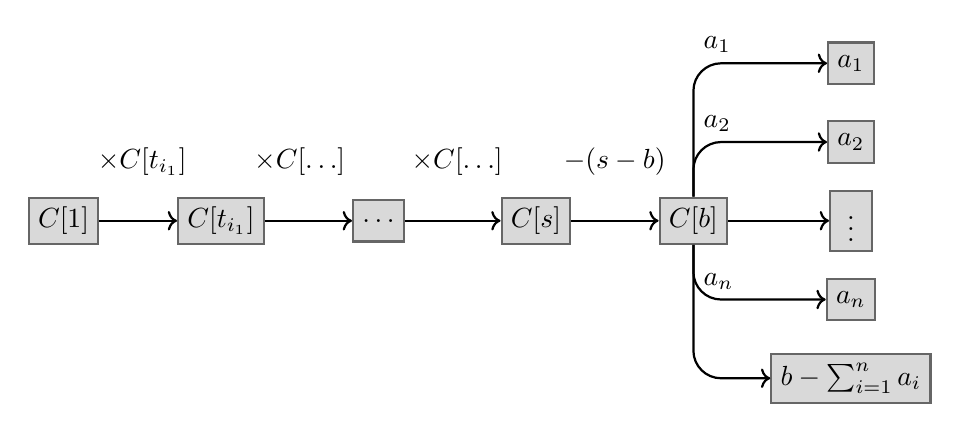
\begin{tikzpicture}[
	t/.style = {rectangle, draw=black!60, fill=black!15, thick, minimum size=15},
	r/.style = {->, thick, rounded corners=10pt}
	]
	
	%Nodes
	\node[t]	(1)		at	(-4, 0)		{$C[1]$};
	\node[t]	(2)		at	(-2, 0)		{$C[t_{i_1}]$};
	\node[t]	(e)		at	(0, 0)		{$\ldots$};
	\node[t]	(s)		at	(2, 0)		{$C[s]$};
	\node[t]	(b)		at	(4, 0)		{$C[b]$};
	
	\node		(t1)	at	(-3, 0.75)	{$\times C[t_{i_1}]$};
	\node		(t2)	at	(-1, 0.75)	{$\times C[\ldots]$};
	\node		(t3)	at	(1, 0.75)	{$\times C[\ldots]$};
	\node		(t4)	at	(3, 0.75)	{$- (s-b)$};
	
	\node[t]	(A1)	at	(6, 2)		{$a_1$};
	\node[t]	(A2)	at	(6, 1)		{$a_2$};
	\node[t]	(Ae)	at	(6, 0)		{$\vdots$};
	\node[t]	(An)	at	(6, -1)		{$a_n$};
	\node[t]	(B)		at	(6, -2)		{$b - \sum_{i=1}^n a_i$};
	
	
	
	%Lines
	\draw[r]	(1.east)	to	(2.west);
	\draw[r]	(2.east)	to	(e.west);
	\draw[r]	(e.east)	to	(s.west);
	\draw[r]	(s.east)	to	(b.west);
	\draw[r]	(b.north)	|-	node[above right]	{$a_1$}	(A1.west);
	\draw[r]	(b.north)	|-	node[above right]	{$a_2$}	(A2.west);
	\draw[r]	(b.east)	to	(Ae.west);
	\draw[r]	(b.south)	|-	node[above right]	{$a_n$}	(An.west);
	\draw[r]	(b.south)	|-	(B.west);
\end{tikzpicture}




\vspace{0.5in}

\noindent Однако, если $s = \prod_{i=1}^k t_{j_i}^{\alpha_i}$ -- то такое решение займёт:

$$
\left( 
k 
\ ; \ 
\prod_{i=1}^k t_{j_i}^{\alpha_i} 
\right)
$$


\noindent Если требуется показать суть зависимости -- то масштабы можно редуцировать до: 

$$\left(x; e^x\right)$$

\

В общем: площадь растёт экспоненциально в зависимости от сложности схемы, что очень неудобно, особенно для сложных базисов.















\newpage

\subsection{Ёлочка}

\

Однако, как мы уже знаем, схемы предыдущего вида можно сократить. первым уровнем аппроксимации упрощения является "ёлочка". Рассмотрим ситуацию $S(b) = b$:

$$\frac{a}{b} = \sum_{i=1}^n \frac{a_i}{s_i} 
\quad \quad
s_i = s_{i-1} \cdot \prod_{j=1}^{k_i} t_{ij}^{\alpha_{ij}}
\quad \quad
s_0 = 1
\quad \quad
a_i < \text{min}(t_{ij})
$$

\

\noindent Пускай, каждый $t_i$ повторяется ровно $\alpha_i$ раз внутри одного $s_i$. Будем реализовывать $s_i$ один за другим:




\vspace{0.5in}

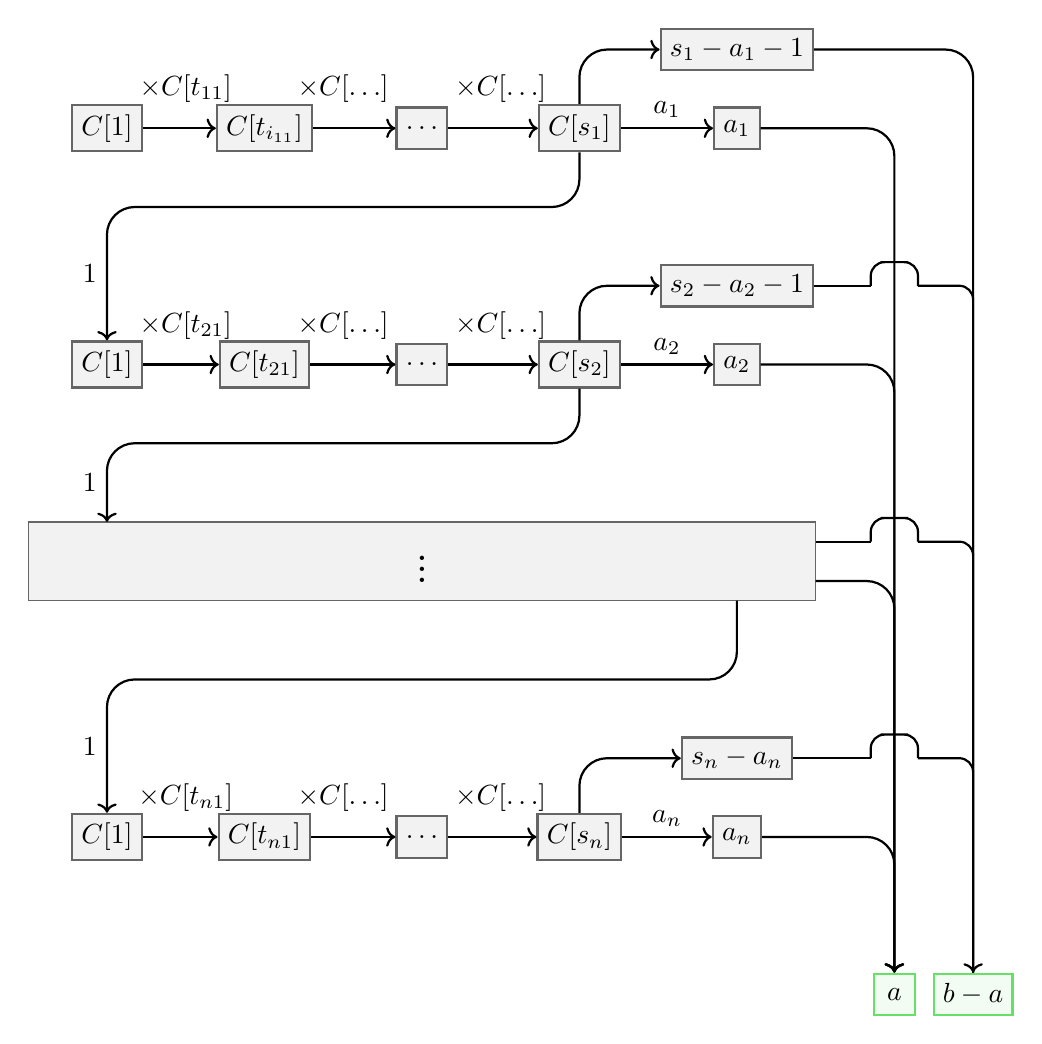
\begin{tikzpicture}[
	o/.style = {rectangle, draw=green!60,	fill=green!5,	thick, minimum size=15},
	t/.style = {rectangle, draw=black!60, 	fill=black!5, 	thick, minimum size=15},
	r/.style = {->, thick, rounded corners=10pt}
	]
	
	% ===== ===== ===== ===== =====
	
	% Nodes
	\node[t]	(11)	at	(-4, 0)		{$C[1]$};
	\node[t]	(12)	at	(-2, 0)		{$C[t_{i_{11}}]$};
	\node[t]	(1e)	at	(0, 0)		{$\ldots$};
	\node[t]	(1s)	at	(2, 0)		{$C[s_1]$};
	
	\node		(1t1)	at	(-3, 0.5)	{$\times C[t_{11}]$};
	\node		(1t2)	at	(-1, 0.5)	{$\times C[\ldots]$};
	\node		(1t3)	at	(1, 0.5)	{$\times C[\ldots]$};
	
	\node[t]	(1B)	at	(4, 1)		{$s_1-a_1-1$};
	\node[t]	(1A)	at	(4, 0)		{$a_1$};
	
	
	
	% Lines
	\draw[r]	(11.east)	to	(12.west);
	\draw[r]	(12.east)	to	(1e.west);
	\draw[r]	(1e.east)	to	(1s.west);
	\draw[r]	(1s.north)	|-	(1B.west);
	\draw[r]	(1s.east)	to	node[above]	{$a_1$}	(1A.west);
	
	
	
	% ===== ===== ===== ===== =====
	
	% Nodes
	\node[t]	(21)	at	(-4, -3)	{$C[1]$};
	\draw[r] (1s.south) |- (-4, -1) to node[left] {$1$} (21.north);
	
	\node[t]	(22)	at	(-2, -3)	{$C[t_{21}]$};
	\node[t]	(2e)	at	(0, -3)		{$\ldots$};
	\node[t]	(2s)	at	(2, -3)		{$C[s_2]$};
	
	\node		(2t1)	at	(-3, -2.5)	{$\times C[t_{21}]$};
	\node		(2t2)	at	(-1, -2.5)	{$\times C[\ldots]$};
	\node		(2t3)	at	(1, -2.5)	{$\times C[\ldots]$};
	
	\node[t]	(2B)	at	(4, -2)		{$s_2-a_2-1$};
	\node[t]	(2A)	at	(4, -3)		{$a_2$};
	
	
	
	% Lines
	\draw[r]	(21.east)	to	(22.west);
	\draw[r]	(22.east)	to	(2e.west);
	\draw[r]	(2e.east)	to	(2s.west);
	\draw[r]	(2s.north)	|-	(2B.west);
	\draw[r]	(2s.east)	to	node[above]	{$a_2$}	(2A.west);
	
	
	
	% ===== ===== ===== ===== ===== 
	\draw[draw=black!60, fill=black!5] (-5, -5) rectangle node {$\textbf{\vdots}$} (5, -6);
	\draw[r] (2s.south) |- (-4, -4) to node[left] {$1$} (-4, -5);
	
	
	
	% ===== ===== ===== ===== =====
	
	% Nodes
	\node[t]	(n1)	at	(-4, -9)	{$C[1]$};
	\draw[r] (4, -6) |- (-4, -7) to node[left] {$1$} (n1.north);
	
	\node[t]	(n2)	at	(-2, -9)	{$C[t_{n1}]$};
	\node[t]	(ne)	at	(0, -9)		{$\ldots$};
	\node[t]	(ns)	at	(2, -9)		{$C[s_n]$};
	
	\node		(nt1)	at	(-3, -8.5)	{$\times C[t_{n1}]$};
	\node		(nt2)	at	(-1, -8.5)	{$\times C[\ldots]$};
	\node		(nt3)	at	(1, -8.5)	{$\times C[\ldots]$};
	
	\node[t]	(nB)	at	(4, -8)		{$s_n-a_n$};
	\node[t]	(nA)	at	(4, -9)		{$a_n$};
	
	
	
	% Lines
	\draw[r]	(n1.east)	to	(n2.west);
	\draw[r]	(n2.east)	to	(ne.west);
	\draw[r]	(ne.east)	to	(ns.west);
	\draw[r]	(ns.north)	|-	(nB.west);
	\draw[r]	(ns.east)	to	node[above]	{$a_n$}	(nA.west);
	
	
	
	% ===== ===== ===== ===== =====
	
	% Nodes
	\node[o]	(out1)	at	(6, -11)	{$a$};
	\node[o]	(out2)	at	(7, -11)	{$b-a$};
	
	% Lines
	\draw[r]	(1A.east)	-|	(out1.north);
	\draw[r]	(2A.east)	-|	(out1.north);
	\draw[r]	(5, -5.75)	-|	(out1.north);
	\draw[r]	(nA.east)	-|	(out1.north);
	
	\draw[r]	(1B.east)	-|	(out2.north);
	
	\draw[thick] (2B.east) to (5.7, -2);
	\draw[thick, rounded corners=5pt] (5.7, -2) |- (6, -1.7) -| (6.3, -2);
	\draw[thick, rounded corners=5pt] (6.3, -2) -| (out2.north);
	
	\draw[thick] (5, -5.25) to (5.7, -5.25);
	\draw[thick, rounded corners=5pt] (5.7, -5.25) |- (6, -4.95) -| (6.3, -5.25);
	\draw[thick, rounded corners=5pt] (6.3, -5.25) -| (out2.north);
	
	\draw[thick] (nB.east) to (5.7, -8);
	\draw[thick, rounded corners=5pt] (5.7, -8) |- (6, -7.7) -| (6.3, -8);
	\draw[thick, rounded corners=5pt] (6.3, -8) -| (out2.north);
	
\end{tikzpicture}




\vspace{0.5in}

Казалось бы, почему "ёлочка", если это "змейка" какая-то? Дело в том, что следует рассмотреть граф, а не алгебраическую схему. Рассмотрим же возможный вид контуров графа:





\vspace{0.5in}

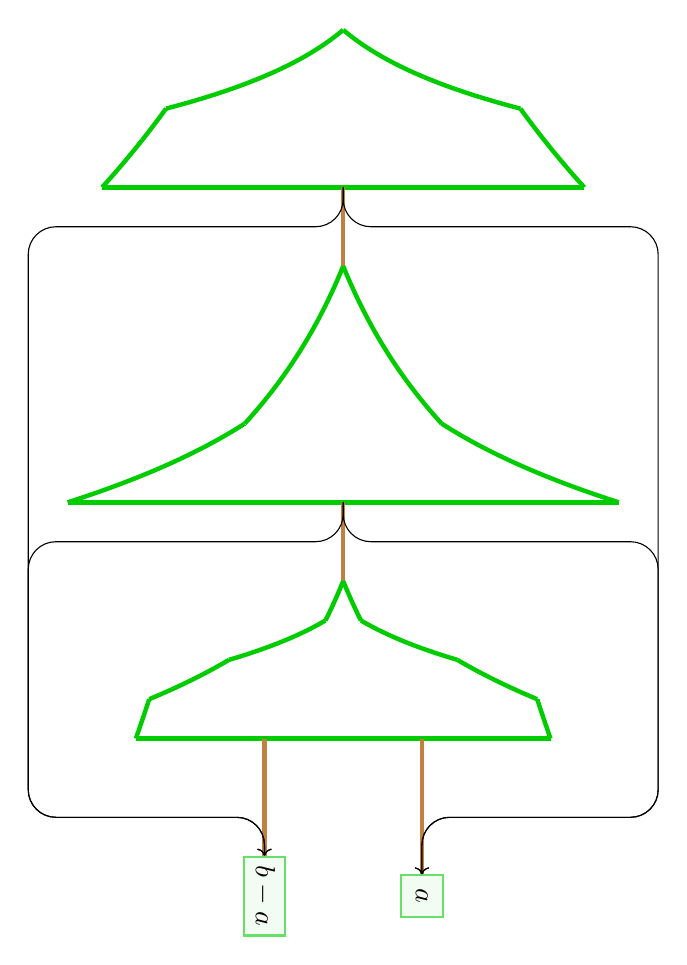
\begin{tikzpicture}[
	rotate=-90,
	o/.style = {rectangle, draw=green!60,	fill=green!5,	thick, minimum size=15},
	r/.style = {->, thin, rounded corners=10pt},
	b/.style = {ultra thick, rounded corners=10pt},
	g/.style = {ultra thick, green}
	]
	
	\begin{axis}[clip = false, 
		hide axis, 
		x=1cm, y=1cm,
		]
		
		\addplot[domain=0:1, g] {3.25^x-1};
		\addplot[domain=1:2, g] {1.25^(x-1)*3.25-1};
		\addplot[domain=0:1, g] {-3.25^x+1};
		\addplot[domain=1:2, g] {-1.25^(x-1)*3.25+1};
		
		\draw[b, green] (axis cs: 2, 3.0625) -- (axis cs:2, -3.0625);
		\draw[b, brown] (axis cs: 2, 0) -- (axis cs: 3, 0);
		
		
		
		\addplot[domain=3:5, g] {1.5^(x-3)-1};
		\addplot[domain=5:6, g] {2^(x-5)*2.25-1};
		\addplot[domain=3:5, g] {-1.5^(x-3)+1};
		\addplot[domain=5:6, g] {-2^(x-5)*2.25+1};
		
		\draw[b, green] (axis cs: 6, 3.5) -- (axis cs:6, -3.5);
		\draw[b, brown] (axis cs: 6, 0) -- (axis cs: 7, 0);
		
		\addplot[domain=7:7.5, g] {1.5^(x-7)-1};
		\addplot[domain=7.5:8, g] {4^(x-7.5)*1.5^0.5-1};
		\addplot[domain=8:8.5, g] {2^(x-8)*1.5^0.5*4^0.5-1};
		\addplot[domain=8.5:9, g] {1.1^(x-8.5)*1.5^0.5*4^0.5*2^0.5-1};
		\addplot[domain=7:7.5, g] {-1.5^(x-7)+1};
		\addplot[domain=7.5:8, g] {-4^(x-7.5)*1.5^0.5+1};
		\addplot[domain=8:8.5, g] {-2^(x-8)*1.5^0.5*4^0.5+1};
		\addplot[domain=8.5:9, g] {-1.1^(x-8.5)*1.5^0.5*4^0.5*2^0.5+1};
		
		\draw[b, green] (axis cs: 9, 2.6332) -- (axis cs: 9, -2.6332);
		
		
		
		\node[o]	(out1)	at	(axis cs: 11, 1)	{$a$};
		\node[o]	(out2)	at	(axis cs: 11, -1)	{$b-a$};
		
		
		
		\draw[b, brown] (axis cs: 9, 1)  to (out1.west);
		\draw[b, brown] (axis cs: 9, -1) to (out2.west);
		\draw[r] (axis cs: 2, 0) -| (axis cs: 2.5, 4)  -- (axis cs: 10, 4)  |- (out1.west);
		\draw[r] (axis cs: 2, 0) -| (axis cs: 2.5, -4) -- (axis cs: 10, -4) |- (out2.west);
		\draw[r] (axis cs: 6, 0) -| (axis cs: 6.5, 4)  -- (axis cs: 10, 4)  |- (out1.west);
		\draw[r] (axis cs: 6, 0) -| (axis cs: 6.5, -4) -- (axis cs: 10, -4) |- (out2.west);
		
		
	\end{axis}
\end{tikzpicture}




\vspace{0.5in}

И действительно: теперь проглядываются "ствол", и крона, которая сначала нарастает-нарастает-нарастает, а затем резко убывает в ноль, и оголяет ствол. И картинка становится похожа на ёлку. 

\

\noindent Так же, такой тип схем занимает меньше места, чем простое дерево: 

$$ 
\sum_{i=1}^{n} 
\left( 
k_i
\ ; \ 
\prod_{j=1}^{k_i} t_{ij}^{\alpha_{ij}} 
\right)
$$

\

\noindent Или, если очень грубо округлять:

$$
\left(
k
\ ; \ 
\text{max}\left(
	\prod_{j=1}^{k_i} t_{ij}^{\alpha_{ij}}
	\right)
\right)
$$

\

Работает это за счёт того, что мы поочерёдно реализуем небольшие степенные деревья, и предварительно успеваем их обрезать, предотвращая экспоненциальный взрыв. Суть та же, что и у линзы френеля. Таким образом, редуцировать размер можно до: 

$$\left(x, e^{x/k}\right)$$

\

Так же, такую схему очень удобно реализовывать в 3D играх: каждую отдельную крону можно выносить на отдельный этаж, что позволит сильно сэкономить вплощади ценой высоты. Однако нарисовать общую схему под произвольное число выходов будет сложно, хотя реализовывать отдельно ничто не запрещает.





















\vspace{1in}

\subsection{Палочка}

\

При всём при этом, можно сократить даже ёлочку: раз у нас $a_i < \text{min}(t_{ij})$ -- то никто нам не гарантирует, что это верно идля остатка -- так что остаток мы и будем скращать. Выберем любое $t_{ij} \ | \ a_i < t_{ij}$, и поставим его в конец очереди для $s_i$:




\vspace{0.5in}

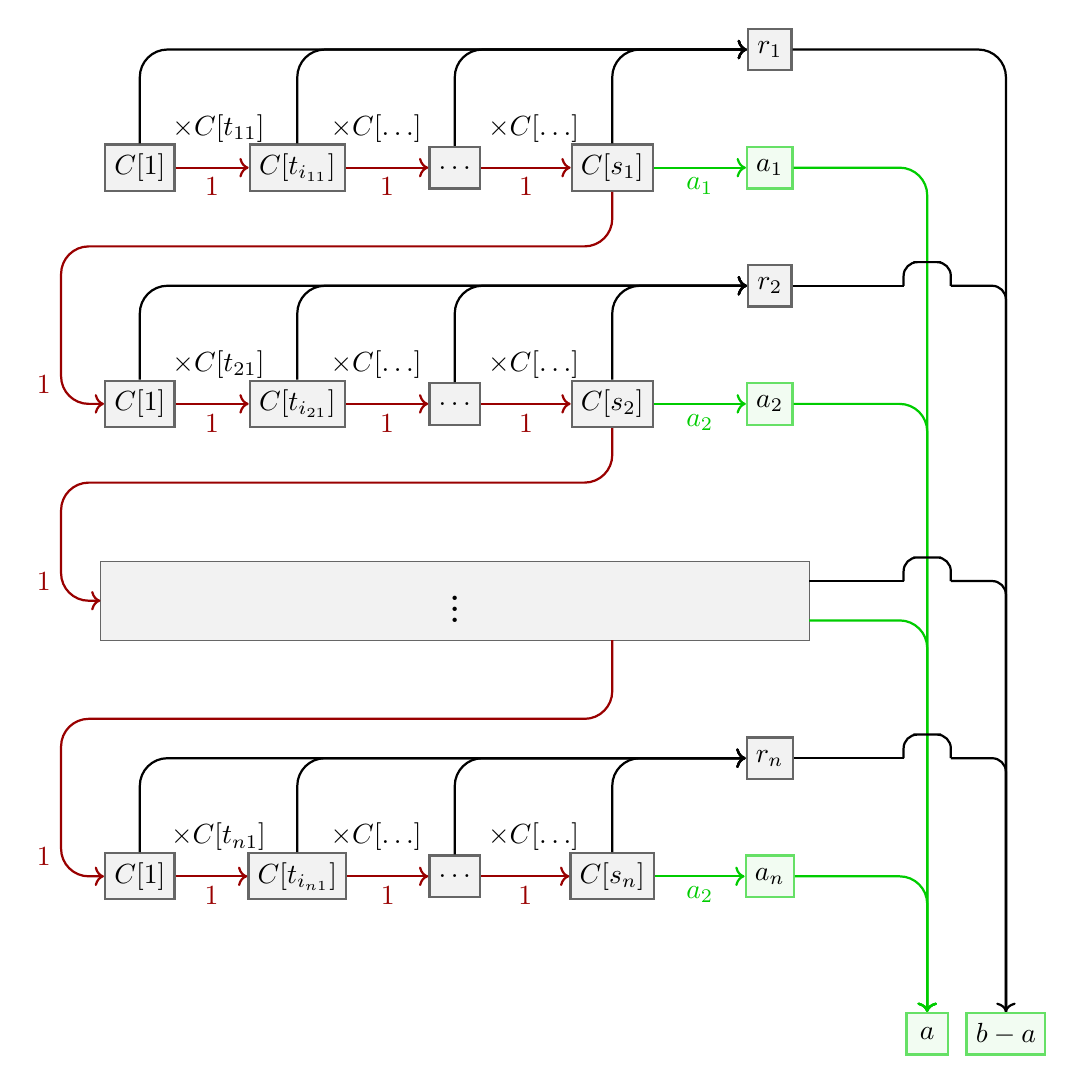
\begin{tikzpicture}[
	o/.style = {rectangle, draw=green!60,	fill=green!5,	thick, minimum size=15},
	t/.style = {rectangle, draw=black!60, 	fill=black!5, 	thick, minimum size=15},
	g/.style = {rectangle, draw=green!60, 	fill=green!5, 	thick, minimum size=15},
	r/.style = {->, thick, rounded corners=10pt}
	]
	
	% ===== ===== ===== ===== =====
	
	% Nodes
	\node[t]	(11)	at	(-4, 0)		{$C[1]$};
	\node[t]	(12)	at	(-2, 0)		{$C[t_{i_{11}}]$};
	\node[t]	(1e)	at	(0, 0)		{$\ldots$};
	\node[t]	(1s)	at	(2, 0)		{$C[s_1]$};
	
	\node		(1t1)	at	(-3, 0.5)	{$\times C[t_{11}]$};
	\node		(1t2)	at	(-1, 0.5)	{$\times C[\ldots]$};
	\node		(1t3)	at	(1, 0.5)	{$\times C[\ldots]$};
	
	\node[g]	(1A)	at	(4, 0)		{$a_1$};
	\node[t]	(1B)	at	(4, 1.5)	{$r_1$};
	
	
	
	% Lines
	\draw[r, red]	(11.east)	to	node[below]	{$1$}	(12.west);
	\draw[r, red]	(12.east)	to	node[below]	{$1$}	(1e.west);
	\draw[r, red]	(1e.east)	to	node[below]	{$1$}	(1s.west);
	\draw[r, green]	(1s.east)	to	node[below]	{$a_1$}	(1A.west);
	\draw[r]	(11.north)	|-	(1B.west);
	\draw[r]	(12.north)	|-	(1B.west);
	\draw[r]	(1e.north)	|-	(1B.west);
	\draw[r]	(1s.north)	|-	(1B.west);
	
	
	
	
	
	% ===== ===== ===== ===== =====
	
	% Nodes
	\node[t]	(21)	at	(-4, -3)	{$C[1]$};
	\draw[r, red] (1s.south) |- (-5, -1) |- node[above left] {$1$} (21.west);
	
	\node[t]	(22)	at	(-2, -3)	{$C[t_{i_{21}}]$};
	\node[t]	(2e)	at	(0, -3)		{$\ldots$};
	\node[t]	(2s)	at	(2, -3)		{$C[s_2]$};
	
	\node		(2t1)	at	(-3, -2.5)	{$\times C[t_{21}]$};
	\node		(2t2)	at	(-1, -2.5)	{$\times C[\ldots]$};
	\node		(2t3)	at	(1, -2.5)	{$\times C[\ldots]$};
	
	\node[g]	(2A)	at	(4, -3)		{$a_2$};
	\node[t]	(2B)	at	(4, -1.5)	{$r_2$};
	
	
	
	% Lines
	\draw[r, red]	(21.east)	to	node[below]	{$1$}	(22.west);
	\draw[r, red]	(22.east)	to	node[below]	{$1$}	(2e.west);
	\draw[r, red]	(2e.east)	to	node[below]	{$1$}	(2s.west);
	\draw[r, green]	(2s.east)	to	node[below]	{$a_2$}	(2A.west);
	\draw[r]	(21.north)	|-	(2B.west);
	\draw[r]	(22.north)	|-	(2B.west);
	\draw[r]	(2e.north)	|-	(2B.west);
	\draw[r]	(2s.north)	|-	(2B.west);
	
	
	
	
	
	% ===== ===== ===== ===== =====
	
	\draw[draw=black!60, fill=black!5] (-4.5, -5) rectangle node {$\textbf{\vdots}$} (4.5, -6);
	\draw[r, red] (2s.south) |- (-5, -4) |- node[above left] {$1$} (-4.5, -5.5);
	
	
	
	
	
	% ===== ===== ===== ===== =====
	
	% Nodes
	\node[t]	(n1)	at	(-4, -9)	{$C[1]$};
	\draw[r, red] (2, -6) |- (-5, -7) |- node[above left] {$1$} (n1.west);
	
	\node[t]	(n2)	at	(-2, -9)	{$C[t_{i_{n1}}]$};
	\node[t]	(ne)	at	(0, -9)		{$\ldots$};
	\node[t]	(ns)	at	(2, -9)		{$C[s_n]$};
	
	\node		(nt1)	at	(-3, -8.5)	{$\times C[t_{n1}]$};
	\node		(nt2)	at	(-1, -8.5)	{$\times C[\ldots]$};
	\node		(nt3)	at	(1, -8.5)	{$\times C[\ldots]$};
	
	\node[g]	(nA)	at	(4, -9)		{$a_n$};
	\node[t]	(nB)	at	(4, -7.5)	{$r_n$};
	
	
	
	% Lines
	\draw[r, red]	(n1.east)	to	node[below]	{$1$}	(n2.west);
	\draw[r, red]	(n2.east)	to	node[below]	{$1$}	(ne.west);
	\draw[r, red]	(ne.east)	to	node[below]	{$1$}	(ns.west);
	\draw[r, green]	(ns.east)	to	node[below]	{$a_2$}	(nA.west);
	\draw[r]	(n1.north)	|-	(nB.west);
	\draw[r]	(n2.north)	|-	(nB.west);
	\draw[r]	(ne.north)	|-	(nB.west);
	\draw[r]	(ns.north)	|-	(nB.west);
	
	
	
	
	
	% ===== ===== ===== ===== =====
	
	% Nodes
	\node[o]	(out1)	at	(6, -11)	{$a$};
	\node[o]	(out2)	at	(7, -11)	{$b-a$};
	
	% Lines
	\draw[r, green]	(1A.east)	-|	(out1.north);
	\draw[r, green]	(2A.east)	-|	(out1.north);
	\draw[r, green]	(4.5, -5.75)-|	(out1.north);
	\draw[r, green]	(nA.east)	-|	(out1.north);
	
	\draw[r]	(1B.east)	-|	(out2.north);
	
	\draw[thick] (2B.east) to (5.7, -1.5);
	\draw[thick, rounded corners=5pt] (5.7, -1.5) |- (6, -1.2) -| (6.3, -1.5);
	\draw[thick, rounded corners=5pt] (6.3, -1.5) -| (out2.north);
	
	\draw[thick] (4.5, -5.25) to (5.7, -5.25);
	\draw[thick, rounded corners=5pt] (5.7, -5.25) |- (6, -4.95) -| (6.3, -5.25);
	\draw[thick, rounded corners=5pt] (6.3, -5.25) -| (out2.north);
	
	\draw[thick] (nB.east) to (5.7, -7.5);
	\draw[thick, rounded corners=5pt] (5.7, -7.5) |- (6, -7.2) -| (6.3, -7.5);
	\draw[thick, rounded corners=5pt] (6.3, -7.5) -| (out2.north);
	
\end{tikzpicture}

\vspace{0.5in}




Забавно, что площадь схем уменьшается, то есть, казалось бы, схемы -- упрощаются -- а наше алгебраическое отоброжение только усложняется... Всё по тому, что увеличивается концентрация решений, а стало быть -- и сложность. Собственно, площадь, занимаемая палочными схемами элементарна:

$$
\left(
k
\ ; \
2
\right)
$$

\

Вау! Линейная площадь! А была ведь экспоненциальная! В чём же подвох? А подвох в том, что данная схема абсолютно не масштабируема. Такие схемы можно реализовывать \textbf{только} для отделения одной величины в случае $S(b) = b$. Если $S(b) \ne b$ -- То палочковую схему построить невозможно... По крайней мере в том виде, что подан в схеме: если повезёт -- придётся избирательно выбирать порядок сплиттеров, а затем избирательно от них забирать конвейеры для возврата. А возможно придётся даже вести несколько параллельных линий, возможно даже с разными порядками действий, или вообще разными сплиттерами впринципе. Если же требуется отделить несколько значений -- то предсказать уже невозможно ничего.

















































































































































\chapter{Медленные системы}

\

Возьмём известную нам "быструю систему", и добавим ограничение на скорость конвейера: введём множество $\mathbb{V}$  допустимых скоростей $v_i$, каждая из которых является вполне конечной. Например, в Satisfactory: 

\noindent $\mathbb{V} = \{60, 120, 270, 480, 720, 1200\}$. Тогда необходимо помимо абстрактной площади начать учитывать и длину конвейеров. А так же необходимо начать учитывать взаимодействие ресурсов и время этого взаимодействия.

\

Обычно, в играх по типу Satisfactory и Factorio "скорость" конвейера измеряется не в метрических единицах $[v_i]$ = м/с, а как пропускная способность $[q_i]$ = шт/с. Но одно можно перевести в другое, если добавить плотность ёмкости конвейера $[\rho_i]$ = шт/м. $v_i \cdot \rho_i = q_i$

\

Однако это всё не меняет допустимый набор действий, а просто накладывает на него некоторые ограничения, и меняет суть задачи: мы перераспределяем не просто ресурсы, а пропускные способности.

$$
\left[
\begin{matrix}
	m_{11} & \ldots & m_{1n} \\
	\vdots & \ddots & \vdots \\
	m_{k1} & \ldots & m_{kn}
\end{matrix}
\right]
\times
\left[
\begin{matrix}
	q^{\text{in}}_1 \\
	\vdots \\
	q^{\text{in}}_n
\end{matrix}
\right]
=
\left[
\begin{matrix}
	q^{\text{out}}_1 \\
	\vdots \\
	q^{\text{out}}_n
\end{matrix}
\right]
$$

\

В матричной форме преобразования, элементы самой матрицы -- скаляры, а элементы векторов -- пропускные способности $[q_i]$ = шт/с

\

Важно отметить, что пропускная способность \underline{конвейера} $q_i$ и пропускная способность \underline{русурсов} $q^{\text{res}}$ -- это две разные, но взаимосвязные вещи: $q^{\text{res}}$ -- это то, что производят заводы, и что "выливается" на конвейеры, которые двигаются с $v_i$, и имеют $\rho_i$. Для адекватной работы такой системы необходимо, чтобы $q^{\text{res}} \le q_i$. В противном случае завод не сможет выкладывать ресурсы на конвейер -- то есть будет простаивать. Таким образом, схемы необходимо проектироавть с учётом этих двух величин.

\

Если же $q^{\text{res}} > q_i$ -- то возможны 2 принципиальные ситуации: $q_i = 0$ и $q_i \ne 0$. Рассмотрим первую на двух примерах:






\vspace{0.25in}
\section{Тупики}







\

\begin{minipage}{0.5\textwidth}
	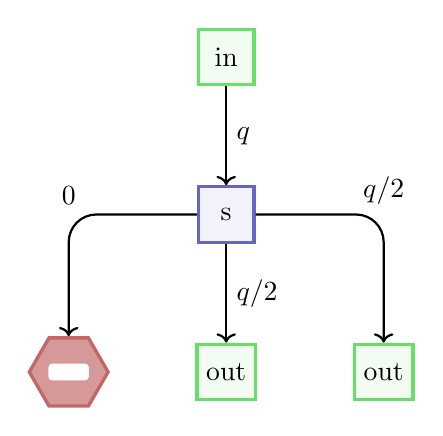
\begin{tikzpicture}[
		s/.style = {rectangle, draw=blue!60,	fill=blue!5,	very thick, minimum size=20},
		a/.style = {rectangle, draw=red!60,		fill=red!5,		very thick, minimum size=20},
		o/.style = {rectangle, draw=green!60,	fill=green!5,	very thick, minimum size=20},
		r/.style = {->, thick, rounded corners=10pt},
		]
		
		% === === Nodes === ===
		\node[o]	(in)	at	(0, 2)	{in};
		\node[s]	(s)		at	(0, 0)	{s};
		\node[o]	(out2)	at	(0, -2)	{out};
		\node[o]	(out3)	at	(2, -2)	{out};
		\node[
			regular polygon, regular polygon sides=6, 
			draw, draw=red!60, fill=red!40, 
			very thick, minimum size=1cm
			] (out1) at (-2, -2) {};
		\draw[
			rounded corners=1.25pt,
			draw, draw=white!100, fill=white!100
			] (-2.25, -2.1) rectangle (-1.75, -1.9);
		
		
		
		% === === Lines === ===
		\draw[r]	(in.south)	to	node[right]	{$q$}	(s.north);
		\draw[r]	(s.west)	-|	node[above]	{$0$}	(out1.north);
		\draw[r]	(s.south)	to	node[right]	{$q/2$}	(out2.north);
		\draw[r]	(s.east)	-|	node[above]	{$q/2$}	(out3.north);
		
	\end{tikzpicture}
\end{minipage}
\begin{minipage}{0.5\textwidth}
	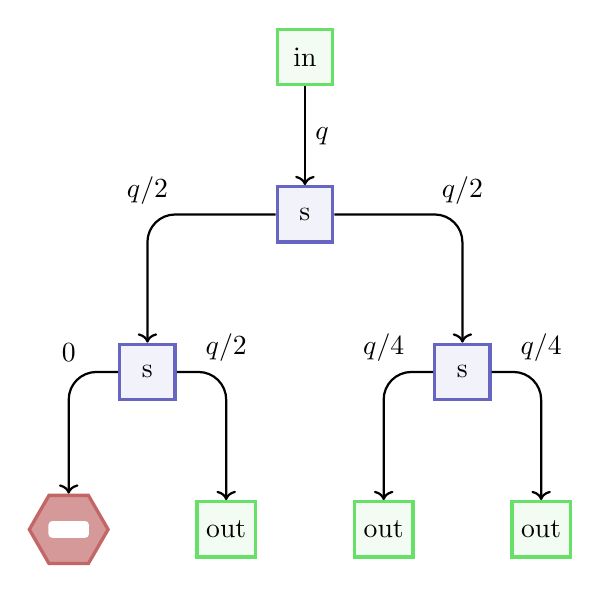
\begin{tikzpicture}[
			s/.style = {rectangle, draw=blue!60,	fill=blue!5,	very thick, minimum size=20},
			a/.style = {rectangle, draw=red!60,		fill=red!5,		very thick, minimum size=20},
			o/.style = {rectangle, draw=green!60,	fill=green!5,	very thick, minimum size=20},
			r/.style = {->, thick, rounded corners=10pt},
			]
			
			% === === Nodes === ===
			\node[o]	(in)	at	(0, 4)		{in};
			\node[s]	(s1)	at	(0, 2)		{s};
			\node[s]	(s2)	at	(-2, 0)		{s};
			\node[s]	(s3)	at	(2, 0)		{s};
			\node[o]	(out2)	at	(-1, -2)	{out};
			
			\node[
				regular polygon, regular polygon sides=6, 
				draw, draw=red!60, fill=red!40, 
				very thick, minimum size=1cm
				] (out1) at (-3, -2) {};
			\draw[
				rounded corners=1.25pt,
				draw, draw=white!100, fill=white!100
				] (-3.25, -2.1) rectangle (-2.75, -1.9);
			
			\node[o]	(out3)	at	(1, -2)	{out};
			\node[o]	(out4)	at	(3, -2)	{out};
			
			
			
			
			% === === Lines === ===
			\draw[r]	(in.south)	to	node[right]	{$q$}	(s1.north);
			\draw[r]	(s1.west)	-|	node[above]	{$q/2$}	(s2.north);
			\draw[r]	(s1.east)	-|	node[above]	{$q/2$}	(s3.north);
			\draw[r]	(s2.west)	-|	node[above]	{$0$}	(out1.north);
			\draw[r]	(s2.east)	-|	node[above]	{$q/2$}	(out2.north);
			\draw[r]	(s3.west)	-|	node[above]	{$q/4$}	(out3.north);
			\draw[r]	(s3.east)	-|	node[above]	{$q/4$}	(out4.north);
		
	\end{tikzpicture}
\end{minipage}






\vspace{0.5in}

Если все конвейеры (кроме тупикового) способны полностью перевозить поданные ресурсы, а спиттеры работают мгновенно -- то сплиттер, подключённый к тупиковой ветке просто уменьшает период своей циклической группы на 1: 

$$C[t_i] \xrightarrow{\text{deadend}} C[t_i-1]$$

\

Таким образом тупик можно интерпретировать, как конвейерный разделитель с нулевым количеством выходов, а следовательно, он -- пустая циклическая группа $C[0]$.

\

Однако важно понимать, что уменьшается период лишь одного сплиттера, а не всей системы целиком, что отлично видно на второй схеме.

\

Благодоря тупиковым ветвям, можно получить преобразование: $\mathbb{T} \to \{ 2, 3 \ldots, \text{max}(\mathbb{T}) \}$, что упрощает построение многих схем.









\vspace{0.25in}
\section{Избыток на выход}

\







\noindent Рассмотрим теперь вторую ситуацию: $q^{\text{res}} > q_i$:

\vspace{0.5in}

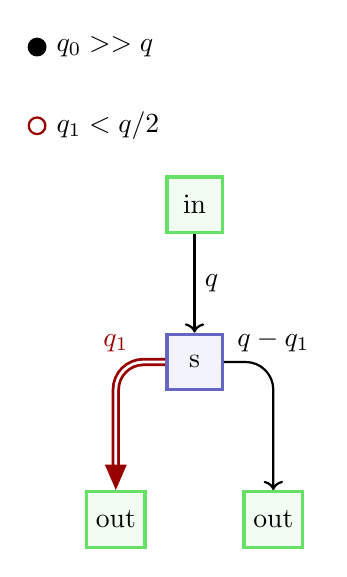
\begin{tikzpicture}[
	s/.style = {rectangle, draw=blue!60,	fill=blue!5,	very thick, minimum size=20},
	a/.style = {rectangle, draw=red!60,		fill=red!5,		very thick, minimum size=20},
	o/.style = {rectangle, draw=green!60,	fill=green!5,	very thick, minimum size=20},
	r/.style = {->, thick, rounded corners=10pt},
	r2/.style = {line width=1pt, 
		double distance=1pt, 
		arrows = {-Stealth[inset=0pt, angle=45:10pt]},
		rounded corners=10pt,
		red
	},
	]
	
	% === === Nodes === ===
	\node[o]	(in)	at	(0, 2)		{in};
	\node[s]	(s)		at	(0, 0)		{s};
	\node[o]	(out1)	at	(-1, -2)	{out};
	\node[o]	(out2)	at	(1, -2)		{out};
	
	\draw[fill=black, thick] (-2,4) circle (3pt) node[right] {$\ q_0>>q$};
	\draw[fill=white, draw=red, thick] (-2,3) circle (3pt) node[right] {$\ q_1 < q/2$};
	
	
	
	% === === Lines === ===
	\draw[r]	(in.south)	to	node[right]	{$q$}	(s.north);
	\draw[r2]	(s.west)	-|	node[above]	{$q_1$}	(out1.north);
	\draw[r]	(s.east)	-|	node[above]	{$q-q_1$}	(out2.north);
	
\end{tikzpicture}



\vspace{0.5in}

Работает данная схема так: если $q_1 \ge q/2$ -- то разделитель работает по обычным правилам. В противном же случае появляется новое правило: разделитель первый цикл работает как $C[t_i]$ вплоть до посещения "критического" выхода. Как только до него доходят -- запускается таймер на $1/q_1$, и пока он не истечёт -- считается, что на этом выходе -- тупик - то есть $C[t_i] \to C[t_i-1]$

\

\noindent Иллюстрация того, \textbf{насколько} сильно может измениться суть схемы, если поставить другой конвейер:




\vspace{0.5in}

\begin{minipage}{0.5\textwidth}
	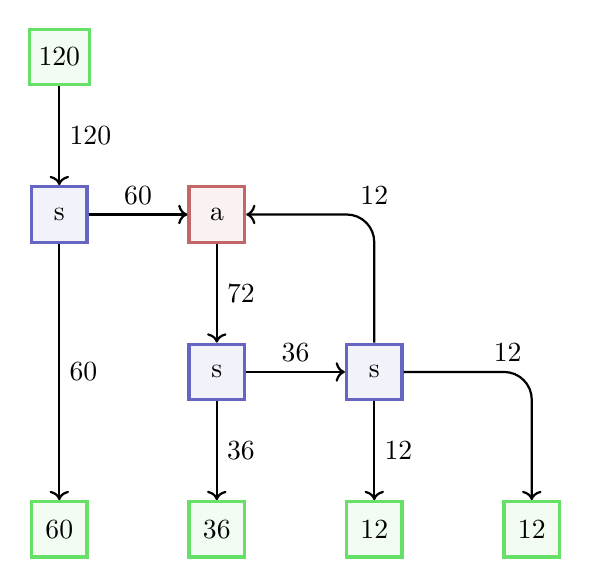
\begin{tikzpicture}[
		s/.style = {rectangle, draw=blue!60,	fill=blue!5,	very thick, minimum size=20},
		a/.style = {rectangle, draw=red!60,		fill=red!5,		very thick, minimum size=20},
		o/.style = {rectangle, draw=green!60,	fill=green!5,	very thick, minimum size=20},
		r/.style = {->, thick, rounded corners=10pt}
		]
		
		
		% === === Nodes === ===
		\node[o]	(in)	at	(0, 4)		{$120$};
		\node[s]	(s)		at	(0, 2)		{s};
		\node[a]	(a)		at	(2, 2)		{a};
		\node[s]	(s1)	at	(2, 0)		{s};
		\node[s]	(s2)	at	(4, 0)		{s};
		\node[o]	(out1)	at	(0, -2)		{$60$};
		\node[o]	(out2)	at	(2, -2)		{$36$};
		\node[o]	(out3)	at	(4, -2)		{$12$};
		\node[o]	(out4)	at	(6, -2)		{$12$};
		
		
		% === === Lines === ===
		\draw[r]	(in.south)	to	node[right]	{$120$}	(s.north);
		\draw[r]	(s.south)	to	node[right]	{$60$}	(out1.north);
		\draw[r]	(s.east)	to	node[above]	{$60$}	(a.west);
		\draw[r]	(a.south)	to	node[right]	{$72$}	(s1.north);
		\draw[r]	(s1.south)	to	node[right]	{$36$}	(out2.north);
		\draw[r]	(s1.east)	to	node[above]	{$36$}	(s2.west);
		\draw[r]	(s2.north)	|-	node[above]	{$12$}	(a.east);
		\draw[r]	(s2.south)	to	node[right]	{$12$}	(out3.north);
		\draw[r]	(s2.east)	-|	node[above left]	{$12$}	(out4.north);
		
		
	\end{tikzpicture}
\end{minipage}
\begin{minipage}{0.5\textwidth}
	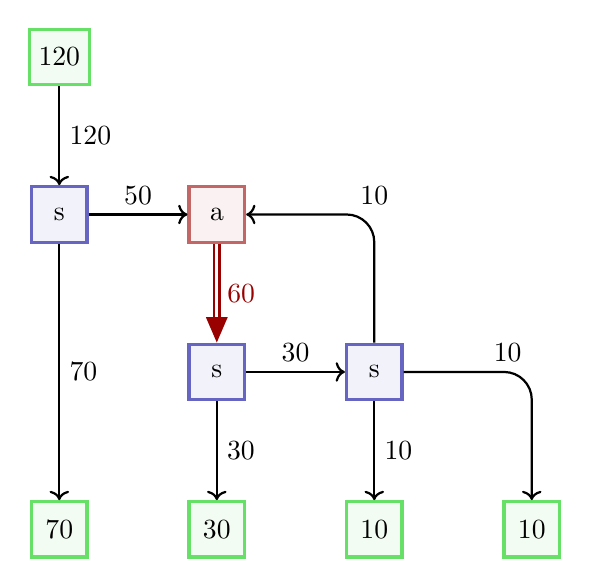
\begin{tikzpicture}[
		s/.style = {rectangle, draw=blue!60,	fill=blue!5,	very thick, minimum size=20},
		a/.style = {rectangle, draw=red!60,		fill=red!5,		very thick, minimum size=20},
		o/.style = {rectangle, draw=green!60,	fill=green!5,	very thick, minimum size=20},
		r/.style = {->, thick, rounded corners=10pt},
		r2/.style = {
			line width=1pt, 
			double distance=1pt, 
			arrows = {-Stealth[inset=0pt, angle=45:10pt]},
			rounded corners=10pt,
			red
		},
		]
		
		
		% === === Nodes === ===
		\node[o]	(in)	at	(0, 4)		{$120$};
		\node[s]	(s)		at	(0, 2)		{s};
		\node[a]	(a)		at	(2, 2)		{a};
		\node[s]	(s1)	at	(2, 0)		{s};
		\node[s]	(s2)	at	(4, 0)		{s};
		\node[o]	(out1)	at	(0, -2)		{$70$};
		\node[o]	(out2)	at	(2, -2)		{$30$};
		\node[o]	(out3)	at	(4, -2)		{$10$};
		\node[o]	(out4)	at	(6, -2)		{$10$};
		
		
		% === === Lines === ===
		\draw[r]	(in.south)	to	node[right]	{$120$}	(s.north);
		\draw[r]	(s.south)	to	node[right]	{$70$}	(out1.north);
		\draw[r]	(s.east)	to	node[above]	{$50$}	(a.west);
		\draw[r2]	(a.south)	to	node[right]	{$60$}	(s1.north);
		\draw[r]	(s1.south)	to	node[right]	{$30$}	(out2.north);
		\draw[r]	(s1.east)	to	node[above]	{$30$}	(s2.west);
		\draw[r]	(s2.north)	|-	node[above]	{$10$}	(a.east);
		\draw[r]	(s2.south)	to	node[right]	{$10$}	(out3.north);
		\draw[r]	(s2.east)	-|	node[above left]	{$10$}	(out4.north);
		
		
	\end{tikzpicture}
\end{minipage}





\vspace{0.5in}

Как видим, такая разница происходит из-за того, что ограниченный конвейер подключенн на выход соединителя. Он превращается в тупик по тем же принципам, что и у сплиттера.

\

Однако сдесь у нас 2 \textbf{взаимосвязанных} конвейера заходят в "бутылочное горлышко", так что скорость основного из них стабилизируется, как единственное решение уравнения

\begin{align*}
	&q_0 \cdot \left( 1 - \frac16 \right) = 60 \\
	&q_0 \cdot \frac65 = 60 \\
	&q_0 = 50
\end{align*}


\

Но тут у нас \textbf{единственное} решение -- а если их несколько? рассмотрим пример, в котором у нас несколько \textbf{независимых} входов:




\vspace{0.5in}

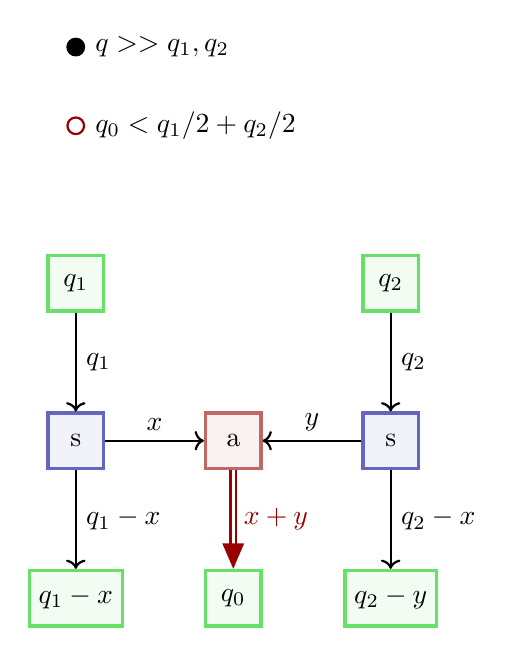
\begin{tikzpicture}[
	s/.style = {rectangle, draw=blue!60,	fill=blue!5,	very thick, minimum size=20},
	a/.style = {rectangle, draw=red!60,		fill=red!5,		very thick, minimum size=20},
	o/.style = {rectangle, draw=green!60,	fill=green!5,	very thick, minimum size=20},
	r/.style = {->, thick, rounded corners=10pt},
	r2/.style = {
		line width=1pt, 
		double distance=1pt, 
		arrows = {-Stealth[inset=0pt, angle=45:10pt]},
		rounded corners=10pt,
		red
	},
	]
	
	\draw[fill=black, thick] (-2,5) circle (3pt) node[right] {$\ q>>q_1, q_2$};
	\draw[fill=white, draw=red, thick] (-2,4) circle (3pt) node[right] {$\ q_0 < q_1/2+q_2/2$};
	
	
	% === === Nodes === ===
	\node[o]	(in1)	at	(-2, 2)		{$q_1$};
	\node[o]	(in2)	at	(2, 2)		{$q_2$};
	\node[s]	(s1)	at	(-2, 0)		{s};
	\node[s]	(s2)	at	(2, 0)		{s};
	\node[a]	(a)		at	(0, 0)		{a};
	\node[o]	(out1)	at	(-2, -2)	{$q_1-x$};
	\node[o]	(out2)	at	(0, -2)		{$q_0$};
	\node[o]	(out3)	at	(2, -2)		{$q_2-y$};
	
	
	% === === Lines === ===
	\draw[r]	(in1.south)	to	node[right]	{$q_1$}		(s1.north);
	\draw[r]	(in2.south)	to	node[right]	{$q_2$}		(s2.north);
	\draw[r]	(s1.south)	to	node[right]	{$q_1-x$}	(out1.north);
	\draw[r]	(s2.south)	to	node[right]	{$q_2-x$}	(out3.north);
	\draw[r]	(s1.east)	to	node[above]	{$x$}		(a.west);
	\draw[r]	(s2.west)	to	node[above]	{$y$}		(a.east);
	\draw[r2]	(a.south)	to	node[right]	{$x+y$}		(out2.north);
	
	
\end{tikzpicture}






\vspace{0.5in}

Очень сильно хочется сказать "пускай $x=y$" -- тогда $x = \frac{q_0}2$. Но на деле нам ничто не гарантирует такого: на деле соединитель может приоритезировать один из входов. Второй случай более интересный: например, в satisfactory есть отдельный тип соеденителя -- приоритетный соединитель (англ: priority merger), в котором есть переключатели степени приоритетности того или иного входа.

\

\noindent Пускай левый вход имеет бóльший приоритет. Рассмотрим возможные ситуации:

\begin{itemize}
	\item $\frac{q_1}2 \le q_0$: $x = \frac{q_1}2$, $y = q_0 - \frac{q_1}2$
	
	\item $\frac{q_1}2 \ge q_0$: $x = q_0$, $y = 0$
\end{itemize}






\vspace{0.5in}

\begin{minipage}{0.333\textwidth}
	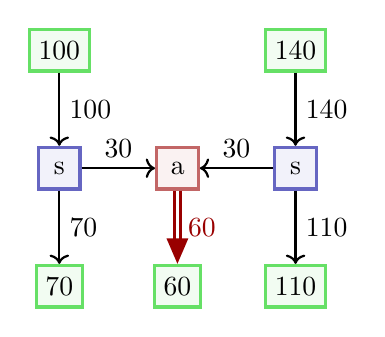
\begin{tikzpicture}[
		s/.style = {rectangle, draw=blue!60,	fill=blue!5,	very thick, minimum size=15},
		a/.style = {rectangle, draw=red!60,		fill=red!5,		very thick, minimum size=15},
		o/.style = {rectangle, draw=green!60,	fill=green!5,	very thick, minimum size=15},
		r/.style = {->, thick, rounded corners=7.5pt},
		r2/.style = {
			line width=1pt, 
			double distance=1pt, 
			arrows = {-Stealth[inset=0pt, angle=45:10pt]},
			rounded corners=7.5pt,
			red
			},
		]
		
		
		% === === Nodes === ===
		\node[o]	(in1)	at	(-1.5, 1.5)		{$100$};
		\node[o]	(in2)	at	(1.5, 1.5)		{$140$};
		\node[s]	(s1)	at	(-1.5, 0)		{s};
		\node[s]	(s2)	at	(1.5, 0)		{s};
		\node[a]	(a)		at	(0, 0)			{a};
		\node[o]	(out1)	at	(-1.5, -1.5)	{$70$};
		\node[o]	(out2)	at	(0, -1.5)		{$60$};
		\node[o]	(out3)	at	(1.5, -1.5)		{$110$};
		
		
		% === === Lines === ===
		\draw[r]	(in1.south)	to	node[right]	{$100$}		(s1.north);
		\draw[r]	(in2.south)	to	node[right]	{$140$}		(s2.north);
		\draw[r]	(s1.south)	to	node[right]	{$70$}		(out1.north);
		\draw[r]	(s2.south)	to	node[right]	{$110$}		(out3.north);
		\draw[r]	(s1.east)	to	node[above]	{$30$}		(a.west);
		\draw[r]	(s2.west)	to	node[above]	{$30$}		(a.east);
		\draw[r2]	(a.south)	to	node[right]	{$60$}		(out2.north);
		
		
	\end{tikzpicture}
\end{minipage}
\begin{minipage}{0.333\textwidth}
	\begin{tikzpicture}[
		s/.style = {rectangle, draw=blue!60,	fill=blue!5,	very thick, minimum size=15},
		a/.style = {rectangle, draw=red!60,		fill=red!5,		very thick, minimum size=15},
		o/.style = {rectangle, draw=green!60,	fill=green!5,	very thick, minimum size=15},
		r/.style = {->, thick, rounded corners=7.5pt},
		r2/.style = {
			line width=1pt, 
			double distance=1pt, 
			arrows = {-Stealth[inset=0pt, angle=45:10pt]},
			rounded corners=7.5pt,
			red
			},
		]
		
		
		% === === Nodes === ===
		\node[o]	(in1)	at	(-1.5, 1.5)		{$100$};
		\node[o]	(in2)	at	(1.5, 1.5)		{$140$};
		\node[s]	(s1)	at	(-1.5, 0)		{s};
		\node[s]	(s2)	at	(1.5, 0)		{s};
		
		\node[
			draw=red!60, fill=red!5, very thick,
			regular polygon, regular polygon sides=3, 
			rotate=-90, minimum size=0.2cm
			] 
			(tri) at (-0.3, 0) {};
		\node[a]	(a)		at	(0, 0)			{p};
		\node				at	(-0.35, 0)		{$1$};
		
		\node[o]	(out1)	at	(-1.5, -1.5)	{$50$};
		\node[o]	(out2)	at	(0, -1.5)		{$60$};
		\node[o]	(out3)	at	(1.5, -1.5)		{$130$};
		
		
		% === === Lines === ===
		\draw[r]	(in1.south)	to	node[right]	{$100$}		(s1.north);
		\draw[r]	(in2.south)	to	node[right]	{$140$}		(s2.north);
		\draw[r]	(s1.south)	to	node[right]	{$50$}		(out1.north);
		\draw[r]	(s2.south)	to	node[right]	{$130$}		(out3.north);
		\draw[r]	(s1.east)	to	node[above]	{$50$}		(tri.south);
		\draw[r]	(s2.west)	to	node[above]	{$10$}		(a.east);
		\draw[r2]	(a.south)	to	node[right]	{$60$}		(out2.north);
		
		
	\end{tikzpicture}
\end{minipage}
\begin{minipage}{0.333\textwidth}
	\begin{tikzpicture}[
		s/.style = {rectangle, draw=blue!60,	fill=blue!5,	very thick, minimum size=15},
		a/.style = {rectangle, draw=red!60,		fill=red!5,		very thick, minimum size=15},
		o/.style = {rectangle, draw=green!60,	fill=green!5,	very thick, minimum size=15},
		r/.style = {->, thick, rounded corners=7.5pt},
		r2/.style = {
			line width=1pt, 
			double distance=1pt, 
			arrows = {-Stealth[inset=0pt, angle=45:10pt]},
			rounded corners=7.5pt,
			red
			},
		]
		
		
		% === === Nodes === ===
		\node[o]	(in1)	at	(-1.5, 1.5)		{$100$};
		\node[o]	(in2)	at	(1.5, 1.5)		{$140$};
		\node[s]	(s1)	at	(-1.5, 0)		{s};
		\node[s]	(s2)	at	(1.5, 0)		{s};
		
		\node[
			draw=red!60, fill=red!5, very thick,
			regular polygon, regular polygon sides=3, 
			rotate=-90, minimum size=0.2cm
			] 
			(tri) at (-0.3, 0) {};
		\node[a]	(a)		at	(0, 0)			{p};
		\node				at	(-0.35, 0)		{$1$};
		
		\node[o]	(out1)	at	(-1.5, -1.5)	{$70$};
		\node[o]	(out2)	at	(0, -1.5)		{$30$};
		\node[o]	(out3)	at	(1.5, -1.5)		{$140$};
		
		
		
		% === === Lines === ===
		\draw[r]	(in1.south)	to	node[right]	{$100$}		(s1.north);
		\draw[r]	(in2.south)	to	node[right]	{$140$}		(s2.north);
		\draw[r]	(s1.south)	to	node[right]	{$70$}		(out1.north);
		\draw[r]	(s2.south)	to	node[right]	{$140$}		(out3.north);
		\draw[r]	(s1.east)	to	node[above]	{$30$}		(tri.south);
		\draw[r]	(s2.west)	to	node[above]	{$0$}		(a.east);
		\draw[r2]	(a.south)	to	node[right]	{$30$}		(out2.north);
		
		
	\end{tikzpicture}
\end{minipage}












\vspace{0.5in}

\begin{tikzpicture}
	\begin{axis}[clip = false,
		xmin = -0.5, xmax = 9, ymin = -0.5, ymax = 4.5, xlabel=$q_1$, x=1cm, y=1cm,
		axis lines = middle, xtick = {4},
		xticklabels = {$2q_0$},
		xticklabel style = {anchor=south west}, 
		xmajorgrids = true,
		ytick = {0}, 
		yticklabels = {},
		grid style = dashed]
		
		
		\addplot[domain=0:4, red, very thick]{x/2};
		\addplot[domain=4:8, red, very thick]{2} node[above, pos=1] {$x$};
		
		\addplot[domain=0:4, blue, very thick]{2-x/2};
		\addplot[domain=4:8, blue, very thick]{0} node[above, pos=1] {$y$};
		
	\end{axis}
\end{tikzpicture}









\vspace{0.5in}

Таким образом приоритетный соединитель работает по следующему алгоритму: когда во вход приходит первый ресурс-- он сразу выходит на конвейер $q$. После этого запускается таймер на $1/q$, на протяжении которого никакие ресурсы не выходят, а просто выстраиваютсяв приоритетную очередь. Когда таймер кончается -- ресурс с бóльшим приоритетом выходит, и заново запускается таймер.

\

\noindent По схожему принципу можно реализовать и другие порядки приоретета, если входов больше двух:

\vspace{0.5in}

\begin{minipage}{0.08\textwidth}
	\begin{tikzpicture}[
		a/.style = {rectangle, draw=red!60,		fill=red!5,		very thick, minimum size=20},
		r/.style = {->, thick, rounded corners=10pt},
		]
		
		
		% === === Nodes === ===				
		\node[
			draw=red!60, fill=red!5, very thick,
			regular polygon, regular polygon sides=3, 
			rotate=-90, minimum size=0.8cm
			] 
			(tri) at (-0.4, 0) {};
		\node				at	(-0.5, 0)		{$1$};
		
		\node[
			draw=red!60, fill=red!5, very thick,
			regular polygon, regular polygon sides=3, 
			rotate=180, minimum size=0.8cm
			] 
			(tri) at (0, 0.4) {};
		\node				at	(0, 0.5)		{$2$};
		
		\node[
			draw=red!60, fill=red!5, very thick,
			regular polygon, regular polygon sides=3, 
			rotate=90, minimum size=0.8cm
			] 
			(tri) at (0.4, 0) {};
		\node				at	(0.5, 0)		{$3$};
		
		
		
		\node[a]	(a)		at	(0, 0)			{p};
		
		
		
		
	\end{tikzpicture}
\end{minipage}
\begin{minipage}{0.05\textwidth}
	$$\equiv$$
\end{minipage}
\begin{minipage}{0.333\textwidth}
	\begin{tikzpicture}[
		a/.style = {rectangle, draw=red!60,		fill=red!5,		very thick, minimum size=15},
		o/.style = {rectangle, draw=green!60,	fill=green!5,	very thick, minimum size=15},
		r/.style = {->, thick, rounded corners=7.5pt},
		]
		
		
		% === === Nodes === ===
		\node[
			draw=red!60, fill=red!5, very thick,
			regular polygon, regular polygon sides=3, 
			rotate=-90, minimum size=0.2cm
			] 
					(tri1)	at	(-0.3, 0)		{};
		\node				at	(-0.35, 0)		{$1$};
		\node[a]	(a1)	at	(0, 0)			{p};
		
		
		\node[
			draw=red!60, fill=red!5, very thick,
			regular polygon, regular polygon sides=3, 
			rotate=-90, minimum size=0.2cm
			] 
					(tri2)	at	(-0.3, -1)		{};
		\node				at	(-0.35, -1)		{$1$};
		\node[a]	(a2)	at	(0, -1)			{p};
		
		
		\node[o]	(in1)	at	(-1, 1)			{3};
		\node[o]	(in2)	at	(-1, 0)			{2};
		\node[o]	(in3)	at	(-1, -1)		{1};
		\node[o]	(out)	at	(0, -2)			{out};
		
		
		
		% === === Lines === ===
		\draw[r]	(in1)		-|	(a1.north);
		\draw[r]	(in2)		to	(tri1.south);
		\draw[r]	(a1.south)	to	(a2.north);
		\draw[r]	(in3)		to	(tri2.south);
		\draw[r]	(a2.south)	to	(out.north);
		
	\end{tikzpicture}
\end{minipage}
\begin{minipage}{0.08\textwidth}
	\begin{tikzpicture}[
		a/.style = {rectangle, draw=red!60,		fill=red!5,		very thick, minimum size=20},
		r/.style = {->, thick, rounded corners=10pt},
		]
		
		
		% === === Nodes === ===				
		\node[
			draw=red!60, fill=red!5, very thick,
			regular polygon, regular polygon sides=3, 
			rotate=-90, minimum size=0.8cm
			] 
			(tri) at (-0.4, 1.5) {};
		\node				at	(-0.45, 1.5)	{$1$};
		
		\node[
			draw=red!60, fill=red!5, very thick,
			regular polygon, regular polygon sides=3, 
			rotate=-90, minimum size=0.8cm
			] 
			(tri) at (-0.4, 0.5) {};
		\node				at	(-0.45, 0.5)	{$2$};
		
		\node[
			draw=red!60, fill=red!5, very thick,
			regular polygon, regular polygon sides=3, 
			rotate=-90, minimum size=0.8cm
			] 
			(tri) at (-0.4, -0.5) {};
		\node				at	(-0.45, -0.45)	{$\vdots$};
		
		\node[
			draw=red!60, fill=red!5, very thick,
			regular polygon, regular polygon sides=3, 
			rotate=-90, minimum size=0.8cm
			] 
			(tri) at (-0.4, -1.5) {};
		\node				at	(-0.45, -1.5)	{$n$};
		
		
		
		\draw[draw=red!60, fill=red!5] (-0.333, 2) rectangle node {p} (0.333, -2);
		
		
		
		
	\end{tikzpicture}
\end{minipage}
\begin{minipage}{0.05\textwidth}
	$$\equiv$$
\end{minipage}
\begin{minipage}{0.1\textwidth}
	\begin{tikzpicture}[
		a/.style = {rectangle, draw=red!60,		fill=red!5,		very thick, minimum size=15},
		o/.style = {rectangle, draw=green!60,	fill=green!5,	very thick, minimum size=15},
		r/.style = {->, thick, rounded corners=7.5pt},
		]
		
		
		% === === Nodes === ===
		\node[
			draw=red!60, fill=red!5, very thick,
			regular polygon, regular polygon sides=3, 
			rotate=-90, minimum size=0.2cm
			] 
					(tri1)	at	(-0.3, 0)		{};
		\node				at	(-0.35, 0)		{$1$};
		\node[a]	(a1)	at	(0, 0)			{p};
		
		
		\node[
			draw=red!60, fill=red!5, very thick,
			regular polygon, regular polygon sides=3, 
			rotate=-90, minimum size=0.2cm
			] 
					(tri2)	at	(-0.3, -1)		{};
		\node				at	(-0.35, -1)		{$1$};
		\node[a]	(a2)	at	(0, -1)			{p};
		
		
		\node[
			draw=red!60, fill=red!5, very thick,
			regular polygon, regular polygon sides=3, 
			rotate=-90, minimum size=0.2cm
			] 
					(tri3)	at	(-0.3, -2)		{};
		\node				at	(-0.35, -2)		{$1$};
		\node[a]	(a3)	at	(0, -2)			{p};
		
		
		\node[o]	(in1)	at	(-1, 1)			{$n$};
		\node[o]	(in2)	at	(-1, 0)			{$\vdots$};
		\node[o]	(in3)	at	(-1, -1)		{2};
		\node[o]	(in4)	at	(-1, -2)		{1};
		\node[o]	(out)	at	(0, -3)			{out};
		
		
		
		% === === Lines === ===
		\draw[r]	(in1)	-|	(a1);
		\draw[r]	(in2)	to	(tri1);
		\draw[r]	(a1)	to	(a2);
		\draw[r]	(in3)	to	(tri2);
		\draw[r]	(a2)	to	(a3);
		\draw[r]	(in4)	to	(tri3);
		\draw[r]	(a3)	to	(out);
		
	\end{tikzpicture}
\end{minipage}







\vspace{0.5in}

При этом так же можно добавить приорететный соединитель, который пускает ресурсы только в рамках заданного соотношения $x:y$ по следующему принципу: без ограничений общности положим, что самый первый ресурс зашёл во вход x. Тогда в этом входе запускается таймер на $\frac{x}{x+y} \cdot \frac1{q}$, а на втором, соответственно -- $\frac{y}{x+y} \cdot \frac1{q}$, на время действия которого данный вход превращается в тупик.

\

\noindent Данную схему также можно реализовать при помощи более простых видов соединителей:





\vspace{0.5in}

\begin{minipage}{0.25\textwidth}
	\begin{tikzpicture}[
		s/.style = {rectangle, draw=blue!60,	fill=blue!5,	very thick, minimum size=15},
		a/.style = {rectangle, draw=red!60,		fill=red!5,		very thick, minimum size=15},
		o/.style = {rectangle, draw=green!60,	fill=green!5,	very thick, minimum size=15},
		r/.style = {->, thick, rounded corners=7.5pt},
		r2/.style = {
			line width=1pt, 
			double distance=1pt, 
			arrows = {-Stealth[inset=0pt, angle=45:10pt]},
			rounded corners=7.5pt,
			red
		},
		]
		
		
		% === === Nodes === ===
		\node[o]	(in1)	at	(-1.5, 1.5)		{$120$};
		\node[o]	(in2)	at	(1.5, 1.5)		{$120$};
		\node[s]	(s1)	at	(-1.5, 0)		{s};
		\node[s]	(s2)	at	(1.5, 0)		{s};
		
		\node[
			draw=red!60, fill=red!5, very thick,
			regular polygon, regular polygon sides=3, 
			rotate=-90, minimum size=0.2cm
			] 
					(tri1)	at	(-0.3, 0)		{};
		\node				at	(-0.35, 0)		{$2$};
		
		\node[
			draw=red!60, fill=red!5, very thick,
			regular polygon, regular polygon sides=3, 
			rotate=90, minimum size=0.2cm
			] 
					(tri2)	at	(0.3, 0)		{};
		\node				at	(0.35, 0)		{$1$};
		
		\node[a]	(a)		at	(0, 0)			{:};
		
		\node[o]	(out1)	at	(-1.5, -1.5)	{$80$};
		\node[o]	(out2)	at	(0, -1.5)		{$60$};
		\node[o]	(out3)	at	(1.5, -1.5)		{$100$};
		
		
		
		% === === Lines === ===
		\draw[r]	(in1)	to	node[right]	{$120$}		(s1);
		\draw[r]	(in2)	to	node[right]	{$120$}		(s2);
		\draw[r]	(s1)	to	node[right]	{$80$}		(out1);
		\draw[r]	(s2)	to	node[right]	{$100$}		(out3);
		\draw[r]	(s1)	to	node[above]	{$40$}		(tri1);
		\draw[r]	(s2)	to	node[above]	{$20$}		(tri2);
		\draw[r2]	(a)		to	node[right]	{$60$}		(out2);
		
		
	\end{tikzpicture}
\end{minipage}
\begin{minipage}{0.1\textwidth}
	$$\equiv$$
\end{minipage}
\begin{minipage}{0.333\textwidth}
	\begin{tikzpicture}[
		s/.style = {rectangle, draw=blue!60,	fill=blue!5,	very thick, minimum size=10},
		a/.style = {rectangle, draw=red!60,		fill=red!5,		very thick, minimum size=10},
		o/.style = {rectangle, draw=green!60,	fill=green!5,	very thick, minimum size=10},
		r/.style = {->, thick, rounded corners=5pt},
		r2/.style = {
			line width=1pt, 
			double distance=1pt, 
			arrows = {-Stealth[inset=0pt, angle=45:10pt]},
			rounded corners=7.5pt,
			red
		},
		]
		
		
		% === === Nodes === ===
		\node[o]	(in1)	at	(-2, 1.5)	{$120$};
		\node[o]	(in2)	at	(1, 1.5)	{$120$};
		\node[s]	(s1)	at	(-2, 0)		{s};
		\node[s]	(s2)	at	(1, 0)		{s};
		\node[s] 	(sa)	at	(-1, 0)		{s};
		
		\node[a]	(a)		at	(0, 0)		{a};
		
		\node[o]	(out1)	at	(-2, -1.5)	{$80$};
		\node[o]	(out2)	at	(0, -1.5)	{$60$};
		\node[o]	(out3)	at	(1, -1.5)	{$100$};
		
		
		
		% === === Lines === ===
		\draw[r]	(in1)	to	node[right]	{$120$}		(s1);
		\draw[r]	(in2)	to	node[right]	{$120$}		(s2);
		\draw[r]	(s1)	to	node[right]	{$80$}		(out1);
		\draw[r]	(s2)	to	node[right]	{$100$}		(out3);
		\draw[r]	(s1)	to	node[above]	{$40$}		(sa);
		\draw[r]	(sa)	to	node[above]	{$20$}		(a);
		
		\draw[r]	(sa)	|-	(-0.5, 0.5)	-|	node[above left]	{$20$}	(a);
		
		\draw[r]	(s2)	to	node[above]	{$20$}		(a);
		\draw[r2]	(a)		to	node[right]	{$60$}		(out2);
		
		
	\end{tikzpicture}
\end{minipage}










\vspace{0.667in}

\begin{minipage}{0.34\textwidth}
	\begin{tikzpicture}[
		s/.style = {rectangle, draw=blue!60,	fill=blue!5,	very thick, minimum size=15},
		a/.style = {rectangle, draw=red!60,		fill=red!5,		very thick, minimum size=15},
		o/.style = {rectangle, draw=green!60,	fill=green!5,	very thick, minimum size=15},
		r/.style = {->, thick, rounded corners=7.5pt},
		r2/.style = {
			line width=1pt, 
			double distance=1pt, 
			arrows = {-Stealth[inset=0pt, angle=45:10pt]},
			rounded corners=7.5pt,
			red
		},
		]
		
		
		% === === Nodes === ===
		\node[o]	(in1)	at	(-2, 2)		{$q_1$};
		\node[o]	(in2)	at	(2, 2)		{$q_2$};
		\node[s]	(s1)	at	(-2, 0)		{s};
		\node[s]	(s2)	at	(2, 0)		{s};
		
		\node[
			draw=red!60, fill=red!5, very thick,
			regular polygon, regular polygon sides=3, 
			rotate=-90, minimum size=0.2cm
			] 
					(tri1)	at	(-0.3, 0)	{};
		\node				at	(-0.35, 0)	{$x$};
		
		\node[
			draw=red!60, fill=red!5, very thick,
			regular polygon, regular polygon sides=3, 
			rotate=90, minimum size=0.2cm
			] 
					(tri2)	at	(0.3, 0)	{};
		\node				at	(0.35, 0)	{$y$};
		
		\node[a]	(a)		at	(0, 0)		{:};
		
		\node[o]	(out1)	at	(-2, -2)	{$q_1-\frac{x}{x+y} \cdot q$};
		\node[o]	(out2)	at	(0, -2)		{$q$};
		\node[o]	(out3)	at	(2, -2)		{$q_2-\frac{y}{x+y} \cdot q$};
		
		
		
		% === === Lines === ===
		\draw[r]	(in1)	to	node[left]	{$q_1$}		(s1);
		\draw[r]	(in2)	to	node[right]	{$q_2$}		(s2);
		\draw[r]	(s1)	to	node[left]	{}	(out1);
		\draw[r]	(s2)	to	node[right]	{}	(out3);
		\draw[r]	(s1)	to	node[above]	{$\frac{x}{x+y} \cdot q$}		(tri1);
		\draw[r]	(s2)	to	node[above]	{$\frac{y}{x+y} \cdot q$}		(tri2);
		\draw[r2]	(a)		to	node[right]	{$q$}		(out2);
		
		
	\end{tikzpicture}
\end{minipage}
\begin{minipage}{0.05\textwidth}
	$$\equiv$$
\end{minipage}
\begin{minipage}{0.333\textwidth}
	\begin{tikzpicture}[
		s/.style = {rectangle, draw=blue!60,	fill=blue!5,	very thick, minimum size=10},
		sx/.style ={rectangle, draw=blue!60,	fill=blue!5,	very thick, minimum size=20},
		a/.style = {rectangle, draw=red!60,		fill=red!5,		very thick, minimum size=10},
		o/.style = {rectangle, draw=green!60,	fill=green!5,	very thick, minimum size=10},
		t/.style = {rectangle, draw=black!60,	fill=black!5, 	very thick, minimum size=10},
		r/.style = {->, thick, rounded corners=5pt},
		r2/.style = {
			line width=1pt, 
			double distance=1pt, 
			arrows = {-Stealth[inset=0pt, angle=45:10pt]},
			rounded corners=7.5pt,
			red
		},
		]
		
		
		% === === Nodes === ===
		\node[o]	(in1)	at	(-4, 2)		{$q_1$};
		\node[o]	(in2)	at	(4, 2)		{$q_2$};
		\node[s]	(s1)	at	(-4, 0)		{s};
		\node[s]	(s2)	at	(4, 0)		{s};
		
		\node[sx] 	(s3)	at	(-3, 0)		{S[$x$]};
		\node[t]	(t11)	at	(-2, 2)		{$1$};
		\node[t]	(t12)	at	(-2, 1)		{$2$};
		\node[t]	(t13)	at	(-2, 0)		{$\vdots$};
		\node[t]	(t14)	at	(-2, -1)	{$x$};
		
		\node[sx] 	(s4)	at	(3, 0)		{S[$y$]};
		\node[t]	(t21)	at	(2, 2)		{$1$};
		\node[t]	(t22)	at	(2, 1)		{$2$};
		\node[t]	(t23)	at	(2, 0)		{$\vdots$};
		\node[t]	(t24)	at	(2, -1)		{$y$};
		
		\draw[draw=red!60, fill=red!5] (-0.333, 2.5) rectangle node {a} (0.333, -1.5);
		
		\node[o]	(out1)	at	(-3.5, -3)	{$q_1-\frac{x}{x+y} \cdot q$};
		\node[o]	(out2)	at	(0, -3)		{$q$};
		\node[o]	(out3)	at	(3.5, -3)		{$q_2-\frac{y}{x+y} \cdot q$};
		
		
		
		% === === Lines === ===
		\draw[r]	(in1)	to	node[left]	{$q_1$}				(s1);
		\draw[r]	(in2)	to	node[right]	{$q_2$}				(s2);
		\draw[r]	(s1)	to									(-4, -2.667);
		\draw[r]	(s2)	to									(4, -2.667);
		\draw[r]	(s1)	to									(s3);
		\draw[r]	(s2)	to									(s4);
		
		\draw[r]	(s3)	|-									(t11);
		\draw[r]	(t11)	to	node[above]	{$\frac{q}{x+y}$}	(-0.333, 2);
		\draw[r]	(s3)	|-									(t12);
		\draw[r]	(t12)	to									(-0.333, 1);
		\draw[r]	(s3)	to									(t13);
		\draw[r]	(t13)	to									(-0.333, 0);
		\draw[r]	(s3)	|-									(t14);
		\draw[r]	(t14)	to									(-0.333, -1);
		
		\draw[r]	(s4)	|-									(t21);
		\draw[r]	(t21)	to	node[above]	{$\frac{q}{x+y}$}	(0.333, 2);
		\draw[r]	(s4)	|-									(t22);
		\draw[r]	(t22)	to									(0.333, 1);
		\draw[r]	(s4)	to									(t23);
		\draw[r]	(t23)	to									(0.333, 0);
		\draw[r]	(s4)	|-									(t24);
		\draw[r]	(t24)	to									(0.333, -1);
		
		\draw[r2]	(0, -1.5)	to	node[right]	{$q$}	(out2);
		
		
	\end{tikzpicture}
\end{minipage}














\vspace{0.5in}

\section{Теорема об инверсии}

\

Однако интересно, а что если соединитель не может принять неограниченное количество конвейеров? В реальности как раз так и происходит: в сатисфактори множество числа входов $\mathbb{A} = \{ 2, 3 \}$. 

\

\noindent Теорма: схема для соединителя $(x:y)$ строится, как инверсия отделителя $(x:y)$:

\begin{itemize}
	\item Направление конвейеров реверсируется
	
	\item Соединители заменяются на разъединители
	
	\item Разъединители заменяются на соединители
	
	\item Выходная лента имеет строго ограниченную скорость: $(q < \frac{q_1}2) \land (q < \frac{q_2}2)$
\end{itemize}





\vspace{0.5in}

\begin{minipage}{0.2\textwidth}
	\begin{tikzpicture}[
		s/.style = {rectangle, draw=blue!60, fill=blue!5, very thick, minimum size=10},
		a/.style = {rectangle, draw=red!60, fill=red!5, very thick, minimum size=10},
		o/.style = {rectangle, draw=green!60, fill=green!5, very thick, minimum size=10},
		r/.style = {->, thick, rounded corners=5pt},
		]
		
		%Nodes
		\node[o]	(in)	at	(0, 2)	{$5x$};
		\node[a]	(a1)	at	(0, 1)	{a};
		\node[s]	(s1)	at	(0, 0)	{s};
		\node[s]	(s2)	at	(0, -1)	{s};
		\node[o]	(out1)	at	(0, -2)	{$1x$};
		\node[a]	(a2)	at	(1, -1)	{a};
		\node[o]	(out2)	at	(1, -2)	{$4x$};
		
		%Lines
		\draw[r]	(in) 	to	node[left]	{$5x$}	(a1);
		\draw[r]	(a1)	to	node[left]	{$6x$}	(s1);
		\draw[r]	(s1)	to	node[left]	{$3x$}	(s2);
		\draw[r]	(s1)	-|	node[above]	{$3x$}	(a2);
		\draw[r]	(s2)	to	node[above]	{$1x$}	(a2);
		\draw[r]	(s2)	-| (-0.75, 0) |- node[left]	{$1x$}	(a1);
		\draw[r]	(s2)	to	node[left]	{$1x$}	(out1);
		\draw[r]	(a2)	to	node[right]	{$4x$}	(out2);
		
	\end{tikzpicture}
\end{minipage}
\begin{minipage}{0.15\textwidth}
	\begin{tikzpicture}[
		r/.style = {->, thick, rounded corners=7pt},
		]
		
		\draw[r] (-0.6, 0) to (-0.3, 0) to (0, 0.375) to (0.6, -0.375) to (0.9, 0) to (1.2, 0);
		
	\end{tikzpicture}
\end{minipage}
\begin{minipage}{0.2\textwidth}
	\begin{tikzpicture}[
		s/.style = {rectangle, draw=blue!60, fill=blue!5, very thick, minimum size=10},
		a/.style = {rectangle, draw=red!60, fill=red!5, very thick, minimum size=10},
		o/.style = {rectangle, draw=green!60, fill=green!5, very thick, minimum size=10},
		r/.style = {->, thick, rounded corners=5pt},
		r1/.style = {<-, thick, rounded corners=5pt},
		r2/.style = {
			line width=0.6pt, 
			double distance=0.6pt, 
			arrows = {-Stealth[inset=0pt, angle=45:6pt]},
			rounded corners=5pt,
			red
		},
		]
		
		\node[right] (1) at (4, 2) {$1x < \frac{q_1}2 \ , \ 4x < \frac{q_2}2$};
		\draw[fill=black, thick] (4,1) circle (3pt) node[right] {$\ q>>q_1, q_2$};
		\draw[fill=white, draw=red, thick] (4,0) circle (3pt) node[right] {$\ q_0 < q_1/2, q_2/2$};
		
		
		%Nodes
		\node[o]	(in)	at	(0, 2)	{$5x$};
		\node[s]	(a1)	at	(0, 1)	{s};
		\node[a]	(s1)	at	(0, 0)	{a};
		\node[a]	(s2)	at	(0, -1)	{a};
		\node[s]	(out1)	at	(0, -2)	{s};
		\node[s]	(a2)	at	(1, -1)	{s};
		\node[s]	(out2)	at	(1, -2)	{s};
		\node[o]	(in1)	at	(0, -3)	{$q_1$};
		\node[o]	(in2)	at	(1, -3)	{$q_2$};
		\node[o]	(out3)	at	(-2, 2)	{$q_1-x$};
		\node[o]	(out4)	at	(2, 2)	{$q_2-4x$};
		
		
		%Lines
		\draw[r2]	(a1) 	to	node[left]	{$5x$}	(in);
		\draw[r1]	(a1)	to	node[left]	{$6x$}	(s1);
		\draw[r1]	(s1)	to	node[left]	{$3x$}	(s2);
		\draw[r1]	(s1)	-|	node[above]	{$3x$}	(a2);
		\draw[r1]	(s2)	to	node[above]	{$1x$}	(a2);
		\draw[r1]	(s2)	-| (-0.75, 0) |- node[left]	{$1x$}	(a1);
		\draw[r1]	(s2)	to	node[left]	{$1x$}	(out1);
		\draw[r1]	(a2)	to	node[right]	{$4x$}	(out2);
		\draw[r]	(in1)	to	node[left]	{$1x$}	(out1);
		\draw[r]	(in2)	to	node[right]	{$4x$}	(out2);
		\draw[r]	(out1)	-|						(out3);
		\draw[r]	(out2)	-|						(out4);
		
	\end{tikzpicture}
\end{minipage}









\vspace{0.5in}

Как можем заметить, в такой схеме сохраняются даже пропускные способности. При этом разъединители перестают в обязательном порядке делить поровну, поскольку они становятся образом соединителей, которые могут принимать конвейеры в любых соотношениях.

\

Нетрудно понять, что если $\mathbb{A} \not\supset \mathbb{T}$ -- то такое преобразование в прямом виде -- невозможно. Но на основе этого принципа можно построить искомую схему. Обозначим: $s(x+y) = s$, $s - (x+y) = b$, $k\cdot(x+y)$. Реализуем схему для соединения $x+y$ конвейеров, а затем реализуем подсхемы для разделения на $x$, $y$ и $b$ независимо. Так же понадобится промежуточно реализоавть схему для разделения на $2$ (если $2 \not\in \mathbb{T}$):






\newpage

\begin{tikzpicture}[
	s`/.style =	{rectangle,	draw=blue!60,	fill=blue!5,	very thick, minimum size=20},
	s/.style =	{rectangle,	draw=blue!60,	fill=blue!5,	very thick, minimum size=10},
	a/.style =	{rectangle,	draw=red!60,	fill=red!5,		very thick, minimum size=10},
	o/.style =	{rectangle,	draw=green!60,	fill=green!5,	very thick, minimum size=10},
	t/.style =	{rectangle,	draw=black!60,	fill=black!5,	thick, 		minimum size=10, inner sep=1pt},
	r`/.style =	{<-, thick, rounded corners=5pt},
	r/.style =	{->, thick, rounded corners=5pt},
	r2/.style = {
		line width=1pt, 
		double distance=1pt, 
		arrows = {-Stealth[inset=0pt, angle=45:10pt]},
		rounded corners=7.5pt,
		red
	},
	]
	
	% === === Nodes === ===
	\node[o]	(in)	at	(-6, 0)		{$v$};
	\node[s`]	(a1)	at	(-3, 0)		{S[$2$]};
	
	\node[a]	(s1)	at	(-1.75, 0)	{a};
	\node[t]	(t11)	at	(-0.75, 0)	{$1$};
	\node[t]	(t12)	at	(-0.75, -4)	{$2$};
	\node[t]	(t1i)	at	(-0.75, -9)	{$a_{i_1}$};
	
	\node[a]	(s11)	at	(0, 0)		{a};
	\node[t]	(t121)	at	(1, 0)		{$1$};
	\node[t]	(t122)	at	(1, -1)		{$2$};
	\node[t]	(t12e)	at	(1, -2)		{$\vdots$};
	\node[t]	(t12i)	at	(1, -3)		{$a_{i_2}$};
	
	\node[a]	(s21)	at	(0, -4)		{a};
	\node[t]	(t221)	at	(1, -4)		{$1$};
	\node[t]	(t222)	at	(1, -5)		{$2$};
	\node[t]	(t22e)	at	(1, -6)		{$\vdots$};
	\node[t]	(t22i)	at	(1, -7)		{$a_{i_2}$};
	
	\node[a]	(si1)	at	(0, -9)		{a};
	\node[t]	(ti21)	at	(1, -9)		{$1$};
	\node[t]	(ti22)	at	(1, -10)	{$2$};
	\node[t]	(ti2e)	at	(1, -11)	{$\vdots$};
	\node[t]	(ti2i)	at	(1, -12)	{$a_{i_2}$};		
	
	% === === etc === ===
	\draw[draw=red!60,		fill=red!5]		(1.5, 0.5)	rectangle node {$\ldots$} (2, -12.5);
	\draw[draw=black!60,	fill=black!5]	(-1, -7.75)	rectangle node {$\ldots$} (1.25, -8.25);
	
	\node[t]	(t1)	at	(2.5, 0)		{$1$};
	\node[t]	(t2)	at	(2.5, -2)		{$2$};
	\node[t]	(te1)	at	(2.5, -4)		{$\vdots$};
	\node[t]	(tb)	at	(2.5, -6)		{$b$};
	\node[t]	(tb+)	at	(2.7, -8)		{$b+1$};
	\node[t]	(te2)	at	(2.5, -10.2)	{$\vdots$};
	\node[t]	(tn)	at	(2.5, -12)		{$s$};
	
	\node[s`]	(a2)	at	(3, -3)			{S[$b$]};
	\node[t]	(t1`x)	at	(5.5, 0)		{$1$};
	\node[t]	(t2`x)	at	(5.5, -1.7)		{$2$};
	\node[t]	(te`x)	at	(5.5, -3.4)		{$\ldots$};
	\node[t]	(tx)	at	(5.5, -5.1)		{$x$};
	\node[t]	(t1`y)	at	(5.5, -6.8)		{$1$};
	\node[t]	(t2`y)	at	(5.5, -8.5)		{$2$};
	\node[t]	(te`y)	at	(5.5, -10.2)	{$\ldots$};
	\node[t]	(ty)	at	(5.5, -12)		{$y$};
	
	\node[s`]	(ax)	at	(6.5, -2.55)	{S[$x$]};
	\node[s`]	(ay)	at	(6.5, -9.35)	{S[$y$]};
	
	\node[s]	(sx)	at	(8, -2.55)		{s};
	\node[s]	(sy)	at	(8, -9.35)		{s};
	
	\node[o]	(outx)	at	(-6, 2)			{$kx+q_1$};
	\node[o]	(outy)	at	(-6, -2)		{$ky+q_2$};
	
	\node[o]	(inx)	at	(9.5, -2.55)	{$2kx+q_1$};
	\node[o]	(iny)	at	(9.5, -9.35)	{$2ky+q_2$};
	
	
	
	% === === Lines === ===
	\draw[r2]	(a1)		to	node[above]	{$v$}	(in);
	\draw[r`]	(a1)		to	(s1);
	
	\draw[r`]	(s1)		to	(t11);
	\draw[r`]	(s1)		|-	(t12);
	\draw[r`]	(s1)		|-	(-1, -8);
	\draw[r`]	(s1)		|-	(t1i);
	
	\draw[r`]	(t11)		to	(s11);
	\draw[r`]	(s11)		to	(t121);
	\draw[r`]	(s11)		|-	(t122);
	\draw[r`]	(s11)		|-	(t12e);
	\draw[r`]	(s11)		|-	(t12i);
	
	\draw[r`]	(t12)		to	(s21);
	\draw[r`]	(s21)		to	(t221);
	\draw[r`]	(s21)		|-	(t222);
	\draw[r`]	(s21)		|-	(t22e);
	\draw[r`]	(s21)		|-	(t22i);
	
	\draw[r`]	(t1i)		to	(si1);
	\draw[r`]	(si1)		to	(ti21);
	\draw[r`]	(si1)		|-	(ti22);
	\draw[r`]	(si1)		|-	(ti2e);
	\draw[r`]	(si1)		|-	(ti2i);
	
	\draw[r`]	(t121)		to	(1.5, 0);
	\draw[r`]	(t122)		to	(1.5, -1);
	\draw[r`]	(t12e)		to	(1.5, -2);
	\draw[r`]	(t12i)		to	(1.5, -3);
	\draw[r`]	(t221)		to	(1.5, -4);
	\draw[r`]	(t222)		to	(1.5, -5);
	\draw[r`]	(t22e)		to	(1.5, -6);
	\draw[r`]	(t22i)		to	(1.5, -7);
	\draw[r`]	(1.25, -8)	to	(1.5, -8);
	\draw[r`]	(ti21)		to	(1.5, -9);
	\draw[r`]	(ti22)		to	(1.5, -10);
	\draw[r`]	(ti2e)		to	(1.5, -11);
	\draw[r`]	(ti2i)		to	(1.5, -12);
	
	\draw[r`]	(2, 0)		to	(t1);
	\draw[r`]	(2, -2)		to	(t2);
	\draw[r`]	(2, -4)		to	(te1);
	\draw[r`]	(2, -6)		to	(tb);
	\draw[r`]	(2, -8)		to	(tb+);
	\draw[r`]	(2, -10.2)	to	(te2);
	\draw[r`]	(2, -12)	to	(tn);
	
	\draw[r`]	(t1) 		-| 	(a2);
	\draw[r`]	(t2) 		-| 	(a2);
	\draw[r`]	(te1)		-| 	(a2);
	\draw[r`]	(tb)		-| 	(a2);
	
	\draw[r`] 	(a2)		-| 	(4, 1) 		-| (a1);
	
	\draw[r`]	(tb+)		to 	(4.5, -8) 	|- 	(t1`x);
	\draw[r`]	(te2)		to 	(5, -10.2)	|- 	(t2`x);
	\draw[r`]	(te2)		to	(5, -10.2)	|- 	(te`x);
	\draw[r`]	(te2)		to	(5, -10.2)	|-	(tx);
	\draw[r`]	(te2)		to 	(5, -10.2) 	|- 	(t1`y);
	\draw[r`]	(te2)		to 	(5, -10.2)	|- 	(t2`y);
	\draw[r`]	(te2)		to	(te`y);
	\draw[r`]	(tn)		to	(ty);
	
	\draw[r`]	(t1`x)		-|	(ax);
	\draw[r`]	(t2`x)		-|	(ax);
	\draw[r`]	(te`x)		-|	(ax);
	\draw[r`]	(tx)		-|	(ax);
	\draw[r`]	(t1`y)		-|	(ay);
	\draw[r`]	(t2`y)		-|	(ay);
	\draw[r`]	(te`y)		-|	(ay);
	\draw[r`]	(ty)		-|	(ay);
	
	\draw[r`]	(ax)		to	node[above]	{$kx$}	(sx);
	\draw[r`]	(ay)		to	node[above]	{$ky$}	(sy);
	
	\draw[r]	(inx)		to	(sx);
	\draw[r]	(iny)		to	(sy);
	
	\draw[r]	(sx)		|-	(outx);
	\draw[r]	(sy)		|-	(6.5, -13)	-|	(-3, -2)	to	(outy);
	
\end{tikzpicture}








\vspace{0.5in}

Казалось бы, что данная схема очень громоздкая, ведь содержит аш 5 различных подсхем... Наделе все 5, включая схему соединителя -- можно сократить по ранее упомянтм же принципам "ёлочки" и "палочки". А если для какого-нибудь $\alpha \in \{ x, y, b \} \ : \ \exists \ t \in \mathbb{T} \ | \ \alpha < t$ -- то такую схему можно реализовать даже без вовзрата, а с уже известными нам тупиками.

\

Хорошо, схема может и не такая уж и большая, как кажется -- но какой всё же в ней смысл, если для каждых $q_1$ и $q_2$ можно реализовать свой разделитель? Вот именно, что \underline{для каждых $q_1$ и $q_2$} нужно будет реализовывать отдельную схему, а тут -- одна для всех. Например, если ресурсы перевозятся поездами с некоторой задержкой с разных производств на другие разные производства -- то одну эту схему можно использовать для разделения обоих случаев, а не строить две независимые схемы -- Нужно лишь в конце тем, или иным методом сделать распределитель на разные заводы (чем мы займёмся в дальнейших главах).










\vspace{0.5in}

\section{Затворы}

\

Однако важно учесть, что может быть так, что $k\cdot(x+y) \not\in \mathbb{V}$. Обозначив $k\cdot(x+y) = v$. Рассмотрим три возможные ситуации:

\

Если $v < \min(\mathbb{V})$ -- запора происходить не будет, и ресурсы будут просто проскальзывать, и соотношение перестанет сохранятся. Можно реализовать затворный механизм: реализуем схему на возврат некоторой доли $\frac{a}{b}$, а оставшиеся конвейеры соеденим. Тогда необходимо, чтобы:

\

$$
v \cdot \frac{1}{1-\frac{a}{b}} = \min(\mathbb{V})
\quad \quad
\frac{v}{\min(\mathbb{V})} = 1 - \frac{a}{b}
\quad \quad
\frac{a}{b} = \frac{\min(\mathbb{V}) - v}{\min(\mathbb{V})}
$$

$$
a = \frac{\min(\mathbb{V}) - v}{\gcd(\min(\mathbb{V}), v)}
\ , \
b = \frac{\min(\mathbb{V})}{\gcd(\min(\mathbb{V}), v)}
$$



\vspace{0.5in}

\begin{tikzpicture}[
	s/.style = {rectangle, draw=blue!60,	fill=blue!5,	very thick, minimum size=20},
	a/.style = {rectangle, draw=red!60,		fill=red!5,		very thick, minimum size=20},
	o/.style = {rectangle, draw=green!60,	fill=green!5,	very thick, minimum size=20},
	r/.style = {->, thick, rounded corners=10pt},
	r2/.style = {
		line width=1pt, 
		double distance=1pt, 
		arrows = {-Stealth[inset=0pt, angle=45:10pt]},
		rounded corners=10pt,
		red
	},
	]
	
	
	% === === Nodes === ===
	\node[o]	(in)	at	(-4, 0)		{$10$};
	\node[a]	(a1)	at	(-2, 0)		{a};
	\node[s]	(s1)	at	(0, 0)		{s};
	\node[s]	(s2)	at	(2, 0)		{s};
	\node[a]	(a2)	at	(2, 2)		{a};
	\node[o]	(out)	at	(4, -2)		{$10$};
	
	
	
	% === === Lines === ===
	\draw[r]	(in)	to	node[above]			{$10$}	(a1);
	\draw[r2]	(a1)	to	node[above]			{$60$}	(s1);
	\draw[r]	(s1)	to	node[above]			{$30$}	(s2);
	\draw[r]	(s1)	|-	node[above right]	{$30$}	(a2);
	\draw[r]	(s2)	to	node[left]			{$10$}	(a2);
	
	\draw[r]	(s2)	-|	(3, 1)	|-	node[below right]	{$10$}	(a2);
	\draw[r]	(a2)	|-	(0, 3)	-|	node[above right]	{$50$}	(a1);
	
	\draw[r]	(s2)	|-	node[below right]	{$10$}	(out);
	
\end{tikzpicture}








\vspace{0.5in}

Если же $v > \max(\mathbb{V})$ -- то наоборот будет происходить перезапор: соотношение будет сохраняться, но числа на выходах будут другие. Воспользуемя принципом чайника и аксиомой архимеда, и просто разделим входной конвейер на несколько параллельных частей, в каждой из которых $\exists \ u \in \mathbb{V} \ | \ v < u$, к которому применим затворный механизм:

\vspace{0.5in}

\begin{tikzpicture}[
	s/.style = {rectangle, draw=blue!60,	fill=blue!5,	very thick, minimum size=10},
	a/.style = {rectangle, draw=red!60,		fill=red!5,		very thick, minimum size=10},
	o/.style = {rectangle, draw=green!60,	fill=green!5,	very thick, minimum size=10},
	r/.style = {->, thick, rounded corners=5pt},
	r2/.style = {
		line width=1pt, 
		double distance=1pt, 
		arrows = {-Stealth[inset=0pt, angle=45:10pt]},
		rounded corners=7.5pt,
		red
	},
	]
	
	
	% === === Nodes === ===
	\node[s]	(s)		at	(-2, -2)	{s};
	\node[o]	(in)	at	(-4, -2)	{$100$};
	
	\node[a]	(a11)	at	(-1, 0)		{a};
	\node[s]	(s11)	at	(0, 0)		{s};
	\node[s]	(s21)	at	(1, 0)		{s};
	\node[a]	(a21)	at	(1, -1)		{a};
	
	\node[a]	(a12)	at	(-1, -4)	{a};
	\node[s]	(s12)	at	(0, -4)		{s};
	\node[s]	(s22)	at	(1, -4)		{s};
	\node[a]	(a22)	at	(1, -3)		{a};
	
	\node[a]	(a3)	at	(1, -2)		{a};
	\node[o]	(out)	at	(3, -2)		{$100$};
		
	
	
	% === === Lines === ===
	\draw[r]	(in)	to	node[above]			{$100$}	(s);
	\draw[r]	(s)		|-	node[below left]	{$50$}	(a11);
	\draw[r]	(s)		|-	node[above left]	{$50$}	(a12);
	
	
	\draw[r2]	(a11)	to	node[above]			{$60$}	(s11);
	\draw[r]	(s11)	to	node[above]			{$30$}	(s21);
	\draw[r]	(s11)	|-	node[above right]	{$30$}	(a21);
	\draw[r]	(s21)	to	node[left]			{$10$}	(a21);
	
	\draw[r]	(s21)	-|	(1.5, -0.5)	|-	node[above right]	{$10$}	(a21);
	\draw[r]	(s21)	|-	(0, 0.5)	-|	node[above right]	{$10$}	(a11);
	
	\draw[r]	(a21)	to	node[left]			{$50$}	(a3);
	
	
	\draw[r2]	(a12)	to	node[above]			{$60$}	(s12);
	\draw[r]	(s12)	to	node[above]			{$30$}	(s22);
	\draw[r]	(s12)	|-	node[above right]	{$30$}	(a22);
	\draw[r]	(s22)	to	node[left]			{$10$}	(a22);
	
	\draw[r]	(s22)	-|	(1.5, -3.5)	|-	node[below right]	{$10$}	(a22);
	\draw[r]	(s22)	|-	(0, -4.5)	-|	node[below right]	{$10$}	(a12);
	
	
	\draw[r]	(a22)	to	node[left]			{$50$}	(a3);
	\draw[r]	(a3)	to	node[above]			{$100$}	(out);
	
\end{tikzpicture}








\vspace{0.5in}

Последняя ситуация: если $\exists \ m, M \in \mathbb{V} \ | \ m < v < M$ -- то в зависимости от конвретных значений $v$ и $\mathbb{V}$ можно использовать оба предыдущих метода.












































































































\newpage
\thispagestyle{empty}
\mbox{}
\newpage

\chapter{Заметки}

рассмотрим следующую задачу: у нас есть некоторое количество входов, с произвольным входом. Требуется перераспределить их между тем же количеством выходов, так, чтобы на каждом из них был одинаковый поток.

\

Очевидно, для \underline{произвольного} значения входа, решение единственно:


\vspace{0.5in}

\begin{tikzpicture}[
	s/.style = {rectangle, draw=blue!60,	fill=blue!5,	very thick, minimum size=10},
	a/.style = {rectangle, draw=red!60,		fill=red!5,		very thick, minimum size=10},
	o/.style = {rectangle, draw=green!60,	fill=green!5,	very thick, minimum size=10},
	r/.style = {->, thick, rounded corners=5pt}
	]
	
	
	% === === Nodes === ===
	\node[o]	(in1)	at	(-2, 2)		{$q_1$};
	\node[o]	(in2)	at	(-1, 2)		{$q_2$};
	\node[o]	(ine)	at	(0, 2)		{$\ldots$};
	\node[o]	(inn)	at	(1, 2)		{$q_n$};
	
	\node[s]	(s1)	at	(-2, 1)		{s};
	\node[s]	(s2)	at	(-1, 1)		{s};
	\node[s]	(se)	at	(0, 1)		{s};
	\node[s]	(sn)	at	(1, 1)		{s};
	
	\node[a]	(a1)	at	(-2, -2)	{a};
	\node[a]	(a2)	at	(-1, -2)	{a};
	\node[a]	(ae)	at	(0, -2)		{a};
	\node[a]	(an)	at	(1, -2)		{a};
	
	\node[o]	(out1)	at	(-2, -3)	{$x$};
	\node[o]	(out2)	at	(-1, -3)	{$x$};
	\node[o]	(oute)	at	(0, -3)		{$x$};
	\node[o]	(outn)	at	(1, -3)		{$x$};
	
	
	
	% === === Lines === ===
	\draw[r]	(in1.south)	to	(s1.north);
	\draw[r]	(in2.south)	to	(s2.north);
	\draw[r]	(ine.south)	to	(se.north);
	\draw[r]	(inn.south)	to	(sn.north);
	
	\draw[r]	(a1.south)	to	(out1.north);
	\draw[r]	(a2.south)	to	(out2.north);
	\draw[r]	(ae.south)	to	(oute.north);
	\draw[r]	(an.south)	to	(outn.north);
	
	\draw[r]	(s1.south)	to	(a1.north);
	\draw[r]	(s2.south)	to	(a2.north);
	\draw[r]	(se.south)	to	(ae.north);
	\draw[r]	(sn.south)	to	(an.north);
	
	
\end{tikzpicture}
















\newpage
\thispagestyle{empty}
\mbox{}
\newpage

Входы: 4, 8, 10, 18

Выходы: 5, 8, 12, 15

\

$$
\left[
\begin{matrix}
	5 \\ 8 \\ 15 \\ 12
\end{matrix}
\right]
=
\left[
\begin{matrix}
	\frac12 & 0 & 0 & 0 \\
	0 		& 1 & 0 & 0 \\
	\frac12 & 0 & 1	& \frac13 \\
	0		& 0 & 0 & \frac23 \\
\end{matrix}
\right]
\times
\left[
\begin{matrix}
	10 \\ 8 \\ 4 \\ 18
\end{matrix}
\right]
$$

\

$$
\left[
\begin{matrix}
	10 \\ 8 \\ 4 \\ 18
\end{matrix}
\right]
=
\left[
\begin{matrix}
	1 & 0 & \frac13 & 0 \\
	0 & 1 & 0       & 0 \\
	0 & 0 & \frac23	& \frac13 \\
	0 & 0 & 0       & \frac23 \\
\end{matrix}
\right]
\times
\left[
\begin{matrix}
	5 \\ 8 \\ 15 \\ 12
\end{matrix}
\right]
$$

\

$$
\left[
\begin{matrix}
	\frac12 & 0 & \frac16 & 0 \\
	0 		& 1 & 0       & 0 \\
	\frac12 & 0 & \frac16 & \frac23 \\
	0		& 0 & \frac13 & \frac13 \\
\end{matrix}
\right] \ \equiv \ \left[
\begin{matrix}
	\frac23 & 0 & \frac13 & \frac16 \\
	0 		& 1 & 0       & 0 \\
	0       & 0 & 0       & \frac16 \\
	\frac13	& 0 & \frac23 & \frac13 \\
\end{matrix}
\right] \ \equiv \ \left[
\begin{matrix}
	1 & 0 & 0 & 0 \\
	0 & 1 & 0 & 0 \\
	0 & 0 & 1 & 0 \\
	0 & 0 & 0 & 1 \\
\end{matrix}
\right]
$$





\vspace{0.5in}

$$
\left[
\begin{matrix}
	\alpha\beta + \frac{b-\alpha}{a} - \beta \cdot \frac{b-\alpha}{a} & 
	\alpha \cdot \frac{1-\beta b}{1+a-b} + \frac{b-\alpha}{a} - \frac{b-\alpha}{a} \cdot \frac{1-\beta b}{1 + a - b} \\
	1 - \alpha\beta - \frac{b-\alpha}{a} + \beta \cdot \frac{b-\alpha}{a} & 
	1 - \alpha \cdot \frac{1-\beta b}{1+a-b} - \frac{b-\alpha}{a} + \frac{b-\alpha}{a} \cdot \frac{1-\beta b}{1 + a - b}
\end{matrix}
\right]
\ \equiv \
$$

$$
\ \equiv \
\left[
\begin{matrix}
	\alpha\beta + \frac{1-\beta b}{1 + a - b} - \alpha \cdot \frac{1-\beta b}{1 + a - b} & 
	\beta \cdot \frac{b-\alpha}{a} + \frac{1-\beta b}{1+a-b} - \frac{b-\alpha}{a} \cdot \frac{1 - \beta b}{1 + a - b} \\
	1 - \alpha\beta - \frac{1-\beta b}{1 + a - b} + \alpha \cdot \frac{1-\beta b}{1 + a - b} & 
	1 - \beta \cdot \frac{b-\alpha}{a} - \frac{1-\beta b}{1+a-b} + \frac{b-\alpha}{a} \cdot \frac{1 - \beta b}{1 + a - b}
\end{matrix}
\right]
\ \equiv \
$$

$$
\ \equiv \
\left[
\begin{matrix}
	1 & 0 \\
	0 & 1
\end{matrix}
\right]
$$













































































































































%\newpage
%\thispagestyle{empty}
%\mbox{}
%\newpage

%\appendix
%\chapter{Brick factory problem}
\label{appendix:a}

\

\lipsum[1-5]








\end{document}